% Inspired by the template by Dave Stevens - https://github.com/davestevens/Loughborough-University-PhD-Thesis-Template/blob/master/thesis.tex
% A4 paper size selected, default is 11pt font, to change to 12pt use [a4paper, 12pt] as option to documentclass
\documentclass[a4paper]{report}

% Some useful packages for including images, colored font, etc.
\usepackage[dvips]{graphicx}
\usepackage{listings}
\usepackage{color}
\usepackage{url}
\usepackage{fancybox}
\usepackage[backend=biber, style=authoryear]{biblatex}
\usepackage[T1]{fontenc}
\usepackage{parskip}
\usepackage{graphicx}
\usepackage[section]{placeins}
\usepackage[hidelinks]{hyperref}
\usepackage{multirow}
\usepackage{subfig}
\usepackage{booktabs}
\usepackage{array}
\usepackage{rotating}

% Add images path
\graphicspath{ {images/} }

% Set the bibliography file
\addbibresource{references.bib}

\renewcommand*{\nameyeardelim}{\addcomma\space}

% Set margins in all document to 3.5cm as per guidelines for binding
\usepackage[includeheadfoot,margin=3.5cm]{geometry}


% Used to produce headers and footers
%\usepackage{fancyhdr}
%\pagestyle{fancyplain}

% Used for removing title in bibliography sections
%\usepackage{titlesec}

% Line spacing defined at 1 and a half.  It says 1.3 but its 1 and a half. For double spacing use 1.6
\linespread{1.3}

% Setup headers and footers
%\fancyhf{}
%\lhead{\leftmark}
% Center on all pages
%\fancyhead[C]{---Draft---}
% Page number placed on right side on odd pages and left side on even pages
%\fancyfoot[RO, LE] {\thepage}

\begin{document}

% Title, Author, Abstract, Acknowledgement, Table of Content, etc....

% Front Page begins

\thispagestyle{empty}

\fancypage{}{\fbox}

%\thisfancyput{%
\begin{center}

%Substitute with the right information
\Large{
\hfill \begin{tabular}{l}
ITMB \\
%Replace this text with your degree name, e.g., Compute Science, Computing and Management, Information Technology and Management of Business, Compute Science and Mathematics, Compute Science and Artificial Intelligence
COC252 \\
%e.g COC251, COC252, COC253, COC255, COC257, COC800, COD290 
F011321
%Replace this text with your ID number
\end{tabular}
}


%\bigskip
%\bigskip
\vspace*{\fill}

%replace by your Project title
\Large{\textbf{EHR System Modernisation \\
in the Republic of Moldova}}

\vspace*{\fill}

by

\vspace*{\fill}

%Replace by your name
Calin Corcimaru


%Replace by your supervisor's name
\vspace*{\fill}
Supervisor: Dr.\ Georgina Cosma
\vspace*{\fill}

\underline{Department of Computer Science} \\
\underline{Loughborough University}

\vspace*{\fill}
%Delete/Change as appropriate
May 2025

\end{center}
%}

% Front Page ends

%Reset so that next pages do not have a box around them
\fancypage{}{}

%set roman numbering for the initial pages
\pagenumbering{roman}

% Abstract
\chapter*{Abstract}
\addcontentsline{toc}{chapter}{Abstract}
This report outlines the result of a project that addresses a key issue in Moldova's healthcare sector: fragmentation of patient data across multiple healthcare institutions. The lack of a nationally-wide integrated system has resulted in overreliance of paper-based and manual processes, leading to reduced patient care quality and incomplete medical histories. Following initial stakeholder consultations and a review of the relevant literature, the project proposed a patient-focused prototype  that allowed users to collect and manage their patient data. The solution enables document uploading and record creation, automated lab result extraction with multimodal large language models and a controlled sharing mechanism with healthcare practitioners. The prototype was implemented using a Vue frontend and FastAPI backend as a web application that demonstrates the feasibility of a patient-focused solution in Moldova's healthcare sector. Stakeholder feedback was collected throughout the whole development process through a series of live demonstrations, allowing for iterative improvements to the application. Final stakeholder feedback confirms the application's potential to enhance care quality and introduce a patient-centric approach to healthcare in Moldova. Overall, this project aims to contribute to Moldova's digital healthcare transformation and hopes to serve as a foundation for future development and implementation of a real-world service.

\textbf{Keywords:} Personal Health Record, Republic of Moldova, Data Fragmentation, Multimodal Large Language Models, Patient-Centric Healthcare

% Acknowledgements
\chapter*{Acknowledgements}
\addcontentsline{toc}{chapter}{Acknowledgements}
I would like to express my gratitude to my project supervisor, Dr.\ Georgina Cosma, for her invaluable guidance and support throughout this project. Her feedback and encouragement have been crucial in motivating and encouraging me to continue exploring and innovating in my system design and development.

I am also deeply grateful to all the stakeholders who have generously contributed their time and ideas to this project. Their insights into the workings of Moldova's healthcare sector and the digital landscape of healthcare technology have been invaluable in shaping the direction of this project. Their feedback and suggestions have been instrumental in refining the system design and ensuring that it meets the needs of its users and improves the quality of care provided to patients. This ultimately ensured that this project efficiently addresses the real-world challenges faced by the healthcare sector in Moldova.

Next, I would like to extend my appreciation to the Loughborough University staff and faculty who provided all the necessary knowledge and support throughout my studies. This project represents a culmination of everything I have learned during my degree, and I am grateful for the opportunity to apply my skills and knowledge in a practical setting.

Finally, I would like to thank my family and friends, who have always been encouraging me during this project. Their belief in my abilities and support have been a source of motivation and inspiration.

I'd like to dedicate this project to my late grandfather, Ion Corcimaru, who was a well-known doctor in Moldova. His devotion to this field and commitment to saving patient lives have always been a source of inspiration for our family. Even though I'm not pursuing a career in medicine, I hope to honour his legacy by contributing to the improvement of healthcare in Moldova through this project. I hope that my work will help to create a better healthcare system for future generations, just as he did for his patients.


% Set the depth for your table of content
% Currently set at 2 (Chapter, Section, Subsection)
\setcounter{tocdepth}{2}

% Include a table of content
\tableofcontents
\addcontentsline{toc}{chapter}{Table of Contents}

% Include a table of figures
\listoffigures
\addcontentsline{toc}{chapter}{List of Figures}

% Include a table of tables
\listoftables
\addcontentsline{toc}{chapter}{List of Tables}

% List of abbreviations
\chapter*{List of Abbreviations}
\addcontentsline{toc}{chapter}{List of Abbreviations}

\begin{tabular}{p{0.2\textwidth} p{0.7\textwidth}}
API & Application Programming Interface \\
CNAM & Centrul Național de Asigurări în Medicină (National Health Insurance Company) \\
CNPDCP & Centrul Național pentru Protecția Datelor cu Caracter Personal (National Center for Personal Data Protection) \\
EHR & Electronic Health Record \\
EMR & Electronic Medical Record \\
HTTP & Hypertext Transfer Protocol \\
HTTPS & Hypertext Transfer Protocol Secure \\
JSON & JavaScript Object Notation \\
JWT & JSON Web Token \\
LLM & Large Language Model \\
MLLM & Multimodal Large Language Model \\
MFA & Multi-Factor Authentication \\
NLP & Natural Language Processing \\
ORM & Object-Relational Mapping \\
PHR & Personal Health Record \\
SDLC & Software Development Life Cycle \\
SFC & Single File Component \\
SIA AMS & Sistemul informațional automatizat „Asistența Medicală Spitalicească” \\
SPA & Single Page Application \\
SSL & Secure Sockets Layer \\
UML & Unified Modeling Language \\
USMF & Universitatea de Stat de Medicină și Farmacie (State University of Medicine and Pharmacy) \\
UUID & Universally Unique Identifier \\
\end{tabular}

% Glossary
\chapter*{Glossary}
\addcontentsline{toc}{chapter}{Glossary}

\begin{description}
    \item[Application Programming Interface (API)] A set of protocols and tools that allow different software applications to communicate with each other.
    \item[Authentication] The process of verifying the identity of a user.
    \item[Authorisation] The process of determining whether a user has permission to access a resource or perform an action.  
    \item[Backend] The server-side of an application that handles business logic, database operations and API requests.
    \item[Dependency injection] A software engineering design pattern where a function receives the object it depends on from an external source rather than creating it itself.
    \item[Entity-Relationship Diagram (ERD)] A visual representation of the database structure, showing the relationships between different entities.
    \item[Frontend] The client-side of an application that users interact with by using a user interface. 
    \item[Hallucination] A phenomenon in which a large language model generates information that appears to be factual but is incorrect or completety made up.
    \item[Javascript Object Notation (JSON)] An interchange format for structured data representation, often used in APIs to exchange data between a client and a server.
    \item[Object Relational Mapping (ORM)] A programming technique that allows developers to interact with a database by mapping database tables to classes and rows to objects.
    \item[Republican hospital] A tertiary healthcare institution in Moldova that serves as the highest level of specialised medical care in the country.
    \item[Single Page Application (SPA)] A web application that loads a single page and dynamically updates the content as the user interacts with the app.
\end{description}

\chapter{Introduction}\label{chap:introduction}

\section{Background}

The Republic of Moldova is a small country in Eastern Europe that borders Romania and Ukraine, with a current population of 2.4 million people \parencite{mdpop}. Since its independence in 1991, Moldova has faced a number of challenges, including political instability, corruption, and economic difficulties which have left Moldova as one of the poorest countries in Europe \parencite{mdpoverty}. 

Despite these challenges, Moldova has made significant progress in its digital transformation efforts, with the government launching a number of initiatives to modernize its public services and improve the quality of life for its citizens \parencite{mdega}. An example is the Citizen's Government Portal (MCabinet), which allows citizens to access personal information such as `valid identity documents, social contributions and benefits, own properties, information about the family doctor and the health institution where the person is registered, tax payments and other information about the citizen-government relationship' \parencite{mdcabinet}. 

To continue supporting the existing transformation initiatives, Moldova's Cabinet of Ministers has recently approved the `Digital Transformation Strategy of the Republic of Moldova for 2023--2030', which aims to transform the country into a digital society by 2030, with the ultimate goal of having `all public services available in a digitalized format' \parencite{mdstrategy}.

\section{Problem Statement}

The healthcare sector in Moldova has also seen some transformations, with the introduction of a new electronic health record system (EHR) in 15 hospitals across the country in 2017, called `Sistemul informațional automatizat „Asistența Medicală Spitalicească” (SIA AMS)' \parencite{mdehr}. While the system has been successful in helping doctors access patient information more efficiently such as medical history, examinations, test results, and prescriptions, the system hasn't been updated since its inception in 2017 and there are still challenges that need to be addressed in 2024.

The main challenge with the current system lies in the user experience (UX) --- SIA AMS feels old and isn't user-friendly, with a clunky interface that is difficult to navigate, not adhering to modern accesibility standards and only accessible via Internet Explorer or legacy version of Microsoft Edge, with no support for other browsers or devices \parencite{mdehr}. 

Another big challenge with the system is its lack of interoperability within public and private medical institutions due to a lack of a nationally-wide integrated system --- each hospital and clinic have their own, siloed, information system that contains the patient information, with no communication being made between systems in different hospitals \parencite{mdehr}. 

Finally, due to the current economic situation in Moldova, the government has not allocated any funds to upgrade the current or develop new systems, and the hospitals and clinics that use the system do not have the resources to update it themselves.

\section{The Client}

The client, `Nicolae Testemiteanu' State University of Medicine and Pharmacy in Moldova (USMF), is a public university in Chisinau, Moldova, that offers a range of medical programs, including medicine, dentistry and pharmacy \parencite{mduni}. Many of the faculty at USMF are also practicing doctors at hospitals and clinics across Moldova, and have first-hand experience with the current IT systems used in both public and private medical institutions. The USMF faculty members that the student will be interacting with during the project are part of an innovation team that researches potential opportunities to improve the healthcare sector in Moldova through the use of technology. As such, the client has expressed a need for a prototype that can act as a proof of concept for a modern system that could either replace or augment the current system in Moldova.

\section{Project Objectives}

This project aims to initially conduct some research on the current situation of the IT systems used in the healthcare sector in Moldova by interviewing several stakeholders from various healthcare-related institutions. Afterwards, the project will conduct a literature review on the most appropriate technologies and methodologies for developing a modernized EHR system, and an analysis of existing EHR systems to identify their existing functionality. Finally, based on the information gathered, the project will focus on designing and developing a working prototype, based on the requirements gathered and the feasibility of the chosen solution for the Moldovan healthcare sector. The student's hope is that the solution can then be used as a proof of concept to secure funding for a full-scale implementation of the new system in Moldova by the relevant authorities, such as the Ministry of Health.

As such, the objectives of the project are as follows:
\begin{enumerate}   
    \item Identify 2 to 4 stakeholders from various perspectives, such as healthcare institutions in Moldova and patients, that can provide insights into the current IT systems used in the healthcare sector in Moldova.
    \item Conduct interviews with the identified stakeholders to gather information on the current IT systems used in the healthcare sector in Moldova.
    \item Carry out a literature review to research the most appropriate technologies (frontend, backend and database) and project management methodologies for developing a modernized EHR system.
    \item Explore at least 2 existing EHR systems and identify their strengths and weaknesses.
    \item Design and develop a working web or mobile app for an EHR system based on the requirements gathered and the feasibility of the chosen solution for the Moldovan healthcare sector.
    \item Offer the client the prototype to be used as a proof of concept to secure funding for a full-scale implementation of the new system in Moldova.
\end{enumerate}

\chapter{Research and Requirements}

To gain a more complete understanding of the current situation in Moldova, the existing problems and possible needs of the people involved, it is important to start with an analysis to identify the possible key stakeholders for this project. As previously mentioned in the literature review, a diverse group of stakeholders is essential to ensure that the currrent situation is reviewed from multiple perspectives. 

Afterwards, the next step is to utilise the chosen stakeholders to gather as much information as possible from various perspective to ensure that the project is aligned with the needs of both patients and healthcare professionals in Moldova and solves the existing problems.

\section{Stakeholder Analysis}

The student has identified the following possible stakeholders for the project:

\begin{itemize}
    \item Doctors and other medical staff working in hospitals
    \item Department head in a hospital
    \item IT staff members in hospitals
    \item Staff members at CNAM (National Health Insurance Company)
    \item Staff members at the Ministry of Health 
    \item Patients 
\end{itemize}

These stakeholders have been identified so that they can provide a wider picture on the needs and requirements of the project, and to ensure that the project is aligned with the expectations of workers within the healthcare industry in Moldova from multiple perspectives. 

The stakeholders have also been placed in the stakeholder influence-interest grid (which will be discussed in section \ref{sec:stakeholders}) to help the student understand the level of influence and interest that each stakeholder has in the project:

\begin{figure}[ht]
    \centering
    
\includegraphics[scale=0.5]{Stakeholder_analysis1.png}
    \caption{Chosen stakeholders in the stakeholder influence-interest grid}
    \label{fig:stakeholder_analysis1}
\end{figure}

\subsection{Current situation analysis}

Following the analysis, the student has conducted several exploratory interviews with the chosen stakeholders to gather insights into current issues with the IT systems used in Moldova's healthcare sector. The student was able to reach out to every stakeholder, except for staff members at CNAM and the Ministry of Health. 

After the conclusion of the interviews, three main issues and potential solutions have been identified:

\begin{enumerate}
    \item Current EHR system is outdated and only accessible via Internet Explorer or legacy version of Microsoft Edge. A potential solution is to develop a new, modernized version of the existing system (retaining the core functionality) that is accessible via modern browsers, is more user friendly and has future upgrade capabilities.
    \item Lack of interoperability between medical institutions due to a lack of a nationally-wide integrated system. A potential solution is to create a new system that acts as a patient history archive, where patients can upload their own medical records (such as lab tests, previous medical history, etc) and share them with any medical practitioner, regardless of the institution they work at. 
    \item Lack of digitalizion for some systems that still rely on paper-based records or very rudimentary data structures, such as the national transplant registry. A potential solution is digitalized of said system, as is in the case of the transplant registry, that can be accessed by any medical practitioner in Moldova.
\end{enumerate}

Analysing the current issues and potential solutions, the student has determined that the solutions for issues \#1 and \#3 are too complex, as they require a complete overhaul and integration with existing systems. As such, the student has decided to focus on issue \#2, as it is the most feasible and can be implemented within the timeframe of the project. 

Consequently, the stakeholder list has been updated to reflect the changed focus of the project:
\begin{itemize}
    \item Doctors working in hospitals and clinics
    \item Staff members at the Ministry of Health
    \item Staff members at CNAM
    \item Patients that are using both public and private healthcare institutions
    \item Other medical staff members (nurses, pharmacists, etc)
    \item Staff members at CNPDCP (National Center for Personal Data Protection)
\end{itemize}

At the same time, the stakeholder influence-interest grid has been updated to reflect the changes in the project focus:

\begin{figure}[ht]
    \centering
    
\includegraphics[scale=0.5]{Stakeholder_analysis2.png}
    \caption{Updated stakeholders in the stakeholder influence-interest grid}
    \label{fig:stakeholder_analysis2}
\end{figure}

\clearpage

\section{Requirements}

After the new stakeholders were identified, additional interviews were conducted to focus on the requirements for the chosen solution and enough information was gathered from the other stakeholders to identify the main requirements for the project. The student was unable to reach out to the staff members at CNAM, the Ministry of Health and CNDCP - instead legislation and regulations on their websites were reviewed \parencite{CNAM,CNPDCP,ministry}. 

All of the gathered requirements can be found in the appendix (section \ref{sec:requirements}), but the most important requirements have been summarized in the table below:

\begin{table}[h!]
    \centering
    \begin{tabular}{|c|c|p{0.65\textwidth}|}
    \hline
    \textbf{ID} & \textbf{Category}                  & \textbf{Requirement}                                                                \\ \hline
    1   & Non-functional     & The system must be accessible on all modern desktop and mobile-based browsers.       \\ \hline
    2   & Non-functional     & The system must store the data in a secure manner, ensuring that only the patient and the doctor can access the data. \\ \hline
    3   & Document upload                 & The system must allow patients to upload their own medical records in a variety of formats (PDF, DOC, etc). \\ \hline
    4  & Personal cabinet        & The system must display the patient's history in a chronological order in the form of a timeline. \\ \hline
    5   & Personal cabinet        & The patient personal cabinet must provide an overview of the patient's history through 3 main sections: personal information, lab tests, and doctor consultations. \\ \hline
    6  & Personal Cabinet & The system must allow patients to add their own personal information, such as name, date of birth, or address. \\ \hline
    7  & Personal Cabinet & The system must allow patients to add their own allergies and vaccinations. \\ \hline
    8   & Shareable link          & The system must allow the patient to generate a shareable link to provide access to their medical records. \\ \hline
    9   & Doctor view & When shared with the doctor, the system must allow the doctor to only view the patient's history, not edit it. \\ \hline
    10   & Patient medication              & The system must allow patients to enter their current medication including details such as the name of the drug, dosage, frequency and start/end date. \\ \hline
    \end{tabular}
    \caption{Summary of the Most Important Requirements}
\end{table}
    
    
    
    

\chapter{Literature Review}

This chapter will provide a review of the existing literature, which will be used guide the student in their planning and development efforts of the project.

\noindent As such, it will be covering the following areas:
\begin{itemize}
    \item Software development methodologies
    \item Requirement and stakeholder management
    \item Tech stack (backend and frotnend
    )
    \item Large Language Models (LLMs)
    \item PHR Systems
\end{itemize}

\section{Software development methodologies}
\label{sec:methodologies}

\subsection{Software Development Life Cycle}

The Software Development Life Cycle (SDLC) is a process used to guide the development of software applications or systems \parencite{sdlc1}. The SDLC consists of multiple phases, each with its own set of activities and deliverables. \textcite{sdlc2} outline the phases of the SDLC as following:
\begin{enumerate}
    \item \textbf{Requirement gathering and analysis phase} - the requirements are gathered saved in a document. Based on the requirements gathered, a development plan is created.
    \item \textbf{Design phase} - requirements are written in a more technical manner and system desings are created. 
    \item \textbf{Implementation phase} - Actual development of the software occurs in this phase. Additionally, some smaller unit tests may be done during this phase.
    \item \textbf{Testing phase} - may involve multiple types of testing, such as unit testing, integration testing, and system testing. \textcite{testing} describes the different types of tests:
    \begin{itemize}
    \item Unit testing - testing individual units or components of the software.
    \item Integration testing - performed on two or more units combined together, focusing on the interfaces between these components.
    \item System testing - focuses on the `end-to-end quality of the entire system', testing it as a whole.
    \end{itemize}
    \item \textbf{Maintenance phase} - involves the deployment and maintenance of the software. Additionally, this phase may include end-user acceptance testing, to ensure that it meets their needs \parencite{testing}. 
\end{enumerate}

\begin{figure}[ht]
    \centering
    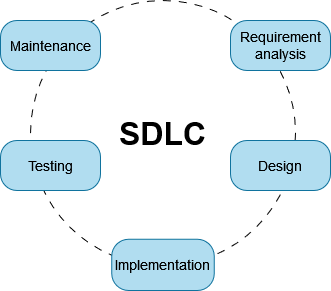
\includegraphics[scale=0.7]{SDLC.png}
    \caption{Software Development Life Cycle}
    \label{fig:sdlc}
\end{figure}

\newpage

\subsection{SDLC Models}

The literature describes several SDLC models that have been used in the development of software applications. \textcite{sdlc1, sdlc2} highlight the most common ones: Waterfall model, V model, Spiral model, Interative model, and Agile model.

\subsubsection{Waterfall Model}

The Waterfall Model is probably the most well-known SDLC model. It is a linear model, where the development process is divided into distinct, sequential phases (which can be seen in figure \ref{fig:waterfall}).

The Waterfall Model's strengths lie in its simplicty of use, ease of understanding and a clear, structured approach \parencite{waterfall}. An additional stregth that the authors note is its extensive documentation and planning, emphasizing quality and adherence to regulations. 

On the other hand, one of Waterfall's main weaknesses is its lack of flexibility in regards to change \parencite{waterfallno}. Thus, this model is not suitable for projects where the requirements are not well understood or are likely to change. Additionally, the project deliverable is not avaialable until the end of the project, any changed or feedback cannot be done during its development \parencite{waterfallno}.

\begin{figure}[ht]
    \centering
    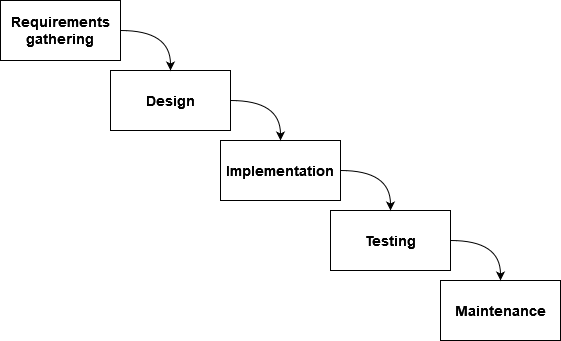
\includegraphics[scale=0.6]{Waterfall.png}
    \caption{Waterfall model}
    \label{fig:waterfall}
\end{figure}

\subsubsection{Agile Model}

Another well-known model is Agile. It has multiple frameworks, with Scrum and Kanban being the most popular ones. Scrum is a framework where the project is divided into sprints, each lasting between 2-4 weeks, that aim on delivering value to the customer through incremental software features \parencite{scrumban, agile}. Kanban focuses on visualizing the project workflow by using a visual board with columns, cards and swimlanes. It uses column limits and a pull system to make the flow of work through the system more efficient \parencite{agile}.

Agile has some drawbacks - its lack of documentation and formal planning, especially in the early stages of the project, may not be suitable for large scale projects \parencite{agile, sdlc2}. Similarly, lack of knowledge on how to use the frameworks may be a barrier for some teams \parencite{waterfallno, sdlc2}.

Nowadays, the combined use of Scrum and Kanban is becoming quite popular, with many teams employing both frameworks in their projects, allowing them to adopt the appropriate practices and adapt them accordingly based on their needs \parencite{scrumban}.

\begin{figure}[ht]
    \centering
    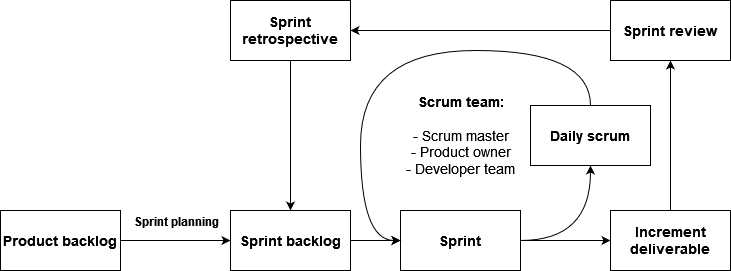
\includegraphics[scale=0.5]{Scrum.png}
    \caption{Scrum framework}
    \label{fig:scrum}
\end{figure}

\subsection{A hybrid approach}

A hybrid approach has also been emerging in software development projects. Various surveys report the most common combinations are Scrum, Iterative Development, Kanban, Waterfall and DevOps, with hybrid Waterfall and Scrum being the most popular one \parencite{hybrid1,hybrid2}. In this approach, the development part is done in an Agile way, with the rest of the project using Waterfall as a backbone \parencite{hybrid2}.

\textcite{hybrid1} note that projects using either Agile, traditional or hybrid approach show similar levels of success in terms of budget, time and quality. However, the authors have found that agile and hybrid approaches perform much better on customer satisfaction than the traditional ones.

\section{Requirements gathering}

Requirements gathering is the first step in any software development process. As described by \textcite{reqanalysis2}, a requirement is a `necessary attribute in a system\ldots that identifies a capability, characteristic, or quality factor of a system in order for it to have value and utility to a user'. Multiple studies mention how proper requirement gathering plays a pivotal role in the project success, with many project failures attributed to poor requirements gathering \parencite{reqanalysis1, reqanalysis3, reqanalysis5}.

\subsection{Requirement types}

Requirements can be classified into 2 categories: functional and non-functional. Functional requirements describe the system's behavior, while non-functional requirements describe the system's quality attributes, such as performance, security, reliability, etc. \parencite[6]{requirements}.

When writing the requirements in a document, it is important to ensure clarity and conciseness to avoid ambiguity. Based on the recommendations of \textcite[112]{requirements} and \textcite{requirements2}, the following principles and practices can be followed:  
\begin{itemize}
    \item Write in a simple and consistent language.
    \item Avoid technical jargon, vague terms, and combining multiple requirements in a single statement.
    \item Ensure that requirements are necessary, appropriate, complete, feasible, and verifiable.
    \item Include attributes for each requirement, such as identification, owner, priority, risk, rationale, difficulty, and type (functional/non-functional).
\end{itemize}

Prioritizing requirements is another crucial task, especially in projects with numerous requirements. Some methods mentioned by \textcite{moscow} include using a low to high priority, assigning a numerical value within a specific range or MoSCoW, which classifies requirements into four categories: 
\begin{itemize}
    \item Must have - must be implemented in the software before being released
    \item Should have - important but not necessary for the software to be released
    \item Could have - desirable but not necessary for the software to be released
    \item Won't have - requirements that are not included in the current release
\end{itemize}

\subsubsection{Requirements in Agile}

In Agile projects, requirements are written in the form of User Stories, which are simple descriptions of a feature desired by the customer, using a specific format: `As a [user], I want to [action] so that [benefit]' \parencite[191]{requirements}. Components of a User Story include a title, acceptance criteria, priority, story points and description. Epics are requirements that cannot be completed in a single sprint and can be broken down into user stories. Epics and User Stories are part of the Product and Sprint backlogs, which contain the requirements for the whole project and the current sprint, respectively.

\subsection{Stakeholders}
\label{sec:stakeholders}

Stakeholders are the individuals who have some interest in the success of the system or project, thus it is important to identify all possible stakeholders in the early stages of the project to avoid missing important requirements or constraints \parencite[34]{requirements}. 

Stakeholder analysis can help understand their position within the project. One way of doing it is by using a stakeholder matrix, such as the Influence/Interest grid (see figure \ref{fig:stakeholder_matrix}), which classifies stakeholders based on their influence and interest in the project \parencite{stakeholders,stakeholders2}.

\begin{figure}[ht]
    \centering
    
\includegraphics[scale=0.5]{Stakeholder.png}
    \caption{Stakeholder Influence/Interest matrix}
    \label{fig:stakeholder_matrix}
\end{figure}

\subsection{Requirement gathering techniques}

Multiple studies mention the most popular requirement gathering techniques are interviews, workshops, prototyping, modelling, brainstorming, storyboards and observing users \parencite{reqanalysis1,reqanalysis2, reqanalysis3, reqanalysis4}. In one of them, individuals with multiple years of experience in requirement gathering were interviewed, and the authors found that the most used techniques were collaborative meetings, interviews, ethnography and modelling \parencite{reqanalysis1}.

Multiple research papers recognise interviews as the most common technique for requirement gathering \parencite{interviews5,interviews1,interviews2}. Some studies have looked at best practices and common mistakes when conducting requirement gathering interviews. The recommended practices, based on \textcite{interviews4, interviews3}, and the common mistakes, from \textcite{interviews1, interviews2}, are summarized in Table \ref{tab:comparison_mistakes_practices} below.

\begin{table}[h!]
    \centering
    \small
    \renewcommand{\arraystretch}{1.2}
    \begin{tabular}{|>{\arraybackslash}m{0.45\textwidth}|>{\arraybackslash}m{0.45\textwidth}|}
    \hline
    \textbf{Common Mistakes} & \textbf{Recommended Practices} \\ \hline
    Wrong opening: failing to understand the context before discussing the problem. & State goals at the beginning and allow customer input at the end. \\ \hline
    Not leveraging ambiguity to reveal knowledge gaps. & Avoid ambiguity by asking clarifying questions. \\ \hline
    Lack of planning: unstructured sequence of questions. & Plan interviews with a structured sequence of questions. \\ \hline
    Failing to build rapport with the customer. & Building rapport through small talk or personal questions in the beginning. \\ \hline
    Implicit goals: failing to ask or clarify stakeholder goals. & Verify alignment and current interpretation with the customer's vision. \\ \hline
    Question omission: not asking about business processes or doing follow-up questions. & Be flexible by probing into relevant topics. \\ \hline
    Weak communication: too much technical jargon usage or not listening to the customer. & Use projective techniques like scenarios to encourage deep thinking. \\ \hline
    Poor question formulation: vague, technical, irrelevant, or too long. & Break down questions or responses into smaller parts and use story telling.  \\ \hline
    Wrong closing sequence: skipping interview summaries or feedback. & Leaving time at the end for the stakeholder to offer any feedback or thoughts. \\ \hline
    \end{tabular}
    \caption{Comparison of Common Mistakes and Recommended Practices}
    \label{tab:comparison_mistakes_practices}
\end{table}

\section{Tech stack}

\subsection{Database}
\label{sec:database}

There are several types of databases, such as: relational (SQL), NoSQL databases, graph databases or object-oriented databases \parencite{databases2}. The choice of database depends on the project or organisation requirements, such as the amount of data, the complexity of the data, the need for scalability, etc. 

\subsubsection{Relational databases}

Relational databases store structured data in tables, linked through keys to create relationships between entries \parencite{databases}. They use SQL (Structured Query Language) to create queries and schemas to help manage data efficiently. \textcite{databases} highlight that relational databases are used, thanks to their high data integrity, for industries like finance and healthcare. Relational databases are widely used, making it easier to find support and resources. However, the rigid schema limits adaptability to rapid data changes or usage of unstructured data. Examples include MySQL, PostgreSQL, Oracle, and Microsoft SQL Server.

\subsubsection{NoSQL databases}

NoSQL databases manage unstructured or semi-structured data without rigid schemas or relationships \parencite{databases}. As the authors describe, NoSQL databases, such as key-value, document, column-family, and graph databases, excel in flexibility and scalability. NoSQL databases often prioritize performance over strict consistency, making them suitable for large datasets of unstructured data but less ideal for complex transactions. NoSQL systems lack SQL’s mature standardization and support. Examples include MongoDB, Cassandra, Couchbase, and Redis.

\subsection{Backend framework}
\label{sec:backend}

Choosing the right backend framework is crucial - it is responsible for handling the business logic of the application, such as processing requests, interacting with the database, and returning responses to the client. A good framework also comes with the added benefit of included features such as security and authentication, database support, a big community and documentation. 

Based on recent a recent survey by \textcite{statista-webframeworks}, the most popular backend frameworks are Express, Flask, Spring Boot, Django and Laravel. This data is also supported by the Stack Overflow Developer Survey 2024, which lists the most popular programming languages as JavaScript (Express), Python (Flask, Django), Java (Spring Boot) and PHP (Laravel) \parencite{stackoverflow}. 

Due to their high popularity among developers, the above frameworks will be compared. Using the information from \textcite{spring,express,django,fastapi}, table \ref{tab:backend} will compare the frameworks based on the following criteria: programming language used, learning curve, community support, security features, database features, and project size suitability.

\begin{table}[h]
    \centering
    \resizebox{\textwidth}{!}{%
    \begin{tabular}{|l|l|l|l|l|}
    \hline
        \textbf{Framework} & \textbf{Django} & \textbf{FastAPI} & \textbf{Spring Boot} & \textbf{Express} \\
    \hline
        \textbf{Language} & Python & Python & Java & JavaScript \\
    \hline
        \textbf{Learning curve} & Medium & Low & High & Low \\
    \hline
        \textbf{Community Support} & High & High & High & High \\
    \hline
        \textbf{Security features} & High & High & High & Medium \\
    \hline
        \textbf{Database features} & Medium & Low & High & Medium \\
    \hline
        \textbf{Project size suitability} & Small to medium & Small to medium & Medium to large & Small to medium \\
    \hline
    \end{tabular}%
    }
    \caption{Comparison of backend frameworks}
    \label{tab:backend}
\end{table}

\subsection{Frontend framework}
\label{sec:frontend}

Similar to the backend frameworks, choosing a suitable frontend framework is equally important - it is responsible for the user interface of the application, such as displaying data, handling user interactions, and making requests to the backend. 

Based on the same survey by \textcite{statista-webframeworks}, the most popular frontend frameworks are React, Angular, Vue.js, and Svelte. This data is also supported by the Stack Overflow Developer Survey 2024, where those frameworks rank among the highest for desirability and admirability among developers \parencite{stackoverflow}.

Table \ref{tab:frontend} will use the information from \textcite{react,angular,vue,svelte} to compare the frameworks based on the following criteria: learning curve, community and documentation, ecosystem and tooling support, performance, state management, and project size suitability.

\begin{table}[h]
    \centering
    \resizebox{\textwidth}{!}{%
    \begin{tabular}{|l|l|l|l|l|}
    \hline
        \textbf{Framework} & \textbf{React} & \textbf{Angular} & \textbf{Vue.js} & \textbf{Svelte} \\ 
    \hline 
        \textbf{Learning curve} & Low & High & Medium & Low \\ 
    \hline
        \textbf{Community and documentation} & High & High & High & Medium \\ 
    \hline
        \textbf{Ecosystem and tooling support} & High & High & Medium & Low \\ 
    \hline
        \textbf{Performance} & High & Medium & Medium & High \\ 
    \hline
        \textbf{State management} & High & High & Medium & Low \\ 
    \hline
        \textbf{Project size suitability} & Small to large & Medium to large & Small to medium & Small to medium \\ 
    \hline
    \end{tabular}%
    }
    \caption{Comparison of frontend frameworks}
    \label{tab:frontend}
\end{table}

\section{Large Language Models (LLMs)}

Large language models (LLMs) are artificial intelligence systems that are used for natural language processing (NLP) tasks such as text generation, translation, summarization and question answering \parencite{llm2,llm_healthcare}. Additionally, LLMs have been found to have emergent capabilities, like reasoning, planning, decision-making and in-contenxt learning \parencite{llm2}. These extraordinary capabilities are achieved through extensive training on large corpus of text data, high parameter count (in the billions) and usage of techniques such as fine-tuning or prompt engineering to improve their performance \parencite{llm2,llm_healthcare}.

LLMs are built on the transformer architecture, which allows them to understand text by learning and remembering the relationships between words \parencite{llm}. These models are first pre-trained on large amounts of unlabeled data using, allowing them to excel in a wide variety of tasks \parencite{foundation, llm2}. These pre-trained models, known as foundation models such as the GPT or Llama families, can then be fine-tuned for specific tasks, improving their performance and accuracy even further \parencite{gpt4,llama3,llm2}.

\subsection{Multimodal LLMs}

One advancement in the field of LLMs has been the addition of multimodal abilities, allowing them to process, understand and generate text and images, audio or videos \parencite{mllm, mllm2}. These new multimodal LLMs (MLLMs) utilise existing reasoning capabilities of LLMs, which are connected to an encoder that can processes images, audio or videos and a generator that helps with generating multimodal outputs \parencite{mllm}. This integration of new modalities allows MLLMs to become versatile tools, expanding their possible use cases and bridging the gap between human and machine interaction \parencite{llm_healthcare}.

\subsubsection{API model providers}

Running and hosting LLMs locally can be a challenge, considering their big model sizes and high computational requirements. As such, many platforms offer APIs that allow users to access LLMs through the cloud. A list of some free API providers, the models offered and their rate limits has been compiled by \textcite{llmapi} and some are listed in the table below.

\begin{table}[h!]
    \centering
    \begin{tabular}{p{2cm} p{5cm} p{6cm}}
        \toprule
        \textbf{Provider} & \textbf{Model name(s)} & \textbf{Free tier limits} \\
        \midrule
        \raggedright
        Groq & Llama 3.2 11B Vision & 7,000 requests/day, 7,000 tokens/minute \\
        & Llama 3.2 90B Vision & 3,500 requests/day, 7,000 tokens/minute \\
        \hline
        \raggedright
        OpenRouter & Llama 3.2 11B Vision Instruct &  \\
        & Llama 3.2 90B Vision Instruct & 20 requests/minute, 200 requests/day \\
        & Gemini 2.0 Flash Experimental &  \\
        \hline
        \raggedright
        Google AI Studio & Gemini 2.0 Flash & 4,000,000 tokens/minute, 10 requests/minute \\
        & Gemini 1.5 Flash & 1,000,000 tokens/minute, 1,500 requests/day, 15 requests/minute \\
        & Gemini 1.5 Pro & 32,000 tokens/minute, 50 requests/day, 2 requests/minute \\
        \hline
        \raggedright
        GitHub Models & OpenAI GPT-4o & Rate limits dependent on Copilot subscription tier \\
        & OpenAI GPT-4o mini & \\
        \hline
        \raggedright
        Cloudflare Workers AI & Llama 3.2 11B Vision Instruct & 10,000 tokens/day \\
        \hline
        \raggedright
        glhf.chat & Any model on Hugging Face that fits on an A100 node (~640GB VRAM)& 480 requests/8 hours \\
        \bottomrule
    \end{tabular}
    \caption{API providers for LLMs}
    \label{tab:llm_apis}
\end{table}

\FloatBarrier
\clearpage

\subsection{LLMs in healthcare}

One application of MLLMs is in healthcare, where the growing volume and complexity of data creates the need for more advanced tools to process and analyze it. LLMs and MLLMs have found use in various healthcare applications, either by using existing models or by developing new, specialized medical models such as Med-PaLm2, BioMistral or Med-Gemini \parencite{biomistral,medgemini,medpalm2}. Some of these applications include:

\begin{itemize}
    \item \textbf{Improving medical diagnosis:} By combining patient records, existing symptoms, and medical history, LLMs can use their reasoning capabilities and memory to assist in diagnosing or preventing health conditions \parencite{llm_healthcare,llm_healthcare3,llm_healthcare4}.
    \item \textbf{Medical Imaging and Multimodal Capabilities:} In diagnostic imaging, multimodal models can assess both text and images (such as X-rays and MRIs) to offer comprehensive analysis. Clinicians can input medical images and contextual information, making MLLMs valuable assistants in the real-time diagnostic processes \parencite{llm_healthcare3}.
    \item \textbf{Virtual Health Assistants:} LLMs can also be deployed as virtual assistants, helping patients with personalised care and general health inquiries \parencite{llm_healthcare,llm_healthcare3}. Patients in areas with limited healthcare access can benefit from these assistants, which also supports healthcare providers by lightening their workloads.
    \item \textbf{Administrative Support:} LLMs can assist in generating Electronic Health Records (EHRs), allowing healthcare providers to focus more on patient interaction \parencite{llm_healthcare4}. Additionally, they can also help translate complex medical terms into more simple language, assist in administrative tasks, and more.
\end{itemize}

\subsection{Prompt Engineering}

The success of LLMs depends not only on the model itself - but also on how it's effectively used by the users, using techniques like prompt engineering, which involves the constant designing and refining of prompts to guide the output of LLMs \parencite{promptmed,prompt2}. Prompts represent instructions given to the model to guide its output, such as providing context, examples, or constraints to the model \parencite{prompt,prompt1,prompt2}. 

There are multiple techniques for prompt engineering, ranging from simple to more advanced. The tables and subsections below outlines some of the most common techniques.

\subsubsection{Zero-Shot Prompting}

Zero-shot prompting are techniques where the LLM is given a prompt without any examples, allowing it to generate an output based on the prompt alone \parencite{prompt1}.

\begin{table}[h!]
    \centering
    \begin{tabular}{p{3cm} p{8cm} p{2cm}}
        \toprule
        \textbf{Technique} & \textbf{Description} & \textbf{Source} \\
        \midrule
        \raggedright
        Role prompting & Assigning a specific role to the LLM in the prompt. The authors note that generally it provides mixed results but may be useful in certain settings.  & \textcite{role1} \\
        \hline
        \raggedright
        Style prompting & Specifying the desired style or tone in the prompt. & \textcite{style} \\
        \hline
        \raggedright
        Emotion prompting & Incorporating phrases of psychological relevance to humans in the prompt. & \textcite{emotion} \\
        \hline
        \raggedright
        Re-reading & Adding the phrase `Read the question again' to the prompt in addition to repeating the question. & \textcite{rereading} \\
        \hline
        \raggedright
        Self-Ask & Prompting the LLM to decide if it needs to ask any follow-up questions for a given prompt. &  \textcite{selfask} \\
        \bottomrule
    \end{tabular}
    \caption{Zero-Shot Prompt Techniques}
    \label{tab:zero_shot}
\end{table}

\FloatBarrier

\subsubsection{Few-Shot Prompting}

Few-shot prompting are techniques where the LLM learns how to complete a task based on a few examples given in the input prompt \parencite{prompt1}.

\begin{table}[h!]
    \centering
    \begin{tabular}{p{3cm} p{8cm} p{2cm}}
        \toprule
        \textbf{Technique} & \textbf{Description} & \textbf{Source} \\
        \midrule
        \raggedright
        Self-Generated In-Context Learning & Using the LLM to automatically generate examples when training/example data is not avaialable. & \textcite{self-generating} \\
        \hline
        \raggedright
        Prompt Mining & Scanning the training data to discover common formats that can be used as prompt templates. & \textcite{mining} \\
        \bottomrule
    \end{tabular}
    \caption{Few-Shot Prompt Techniques}
    \label{tab:few_shot}
\end{table}

\FloatBarrier

\subsubsection{Thought Generation Prompting}

Thought generation are techniques where the prompt encourages the LLM to explain its reasoning process while solving a given problem \parencite{prompt1}.

\begin{table}[h!]
    \centering
    \begin{tabular}{p{3cm} p{8cm} p{2cm}}
        \toprule
        \textbf{Technique} & \textbf{Description} & \textbf{Source} \\
        \midrule
        \raggedright
        Chain-of-Thought (CoT) & Adding a phrase like `Let's think step by step' at the end of the prompt to encourage the LLM to describe its thought process before offering a final answer. & \textcite{cot} \\
        \hline
        \raggedright
        Contrastive CoT & Using CoT and also adding both incorrect and correct examples in order to provide the LLM a more diverse example set.  & \textcite{contrastive-cot} \\
        \hline
        \raggedright
        Auto-CoT & Using CoT with another LLM to automatically generate CoT examples that can be used to create few-shot CoT prompts for other LLMs. &  \textcite{auto-cot} \\
        \hline
        \raggedright
        Least-to-Most & Starts with asking the model to break down a problem into sub-problems without solving them. Afterwards, it solves them one by one, appending the result each time, until it arrives at the answer. & \textcite{least-most} \\
        \hline
        \raggedright
        Tree-of-Thought (ToT) & Starts with an initial problem and then generates multiple possible steps by using CoT. Then, it evaluates each step, decides which one to take and creates more thoughts until it reaches an answer. & \textcite{treeofthought} \\
        \bottomrule
    \end{tabular}
    \caption{Thought Generation Prompt Techniques}
    \label{tab:thought_gen}
\end{table}

\FloatBarrier

\subsubsection{Multimodal and Multilingual Prompting}

Multimodal and multilingual prompting are techniques which aim to improve an LLM's performance by leveraging multiple modalities or languages in the prompt \parencite{prompt1}.

\begin{table}[h!]
    \centering
    \begin{tabular}{p{3cm} p{8cm} p{2cm}}
        \toprule
        \textbf{Technique} & \textbf{Description} & \textbf{Source} \\
        \midrule
        \raggedright
        Translate-first prompting & Translating the input prompt into English to leverage LLMs strengths in dealing with English inputs, compared to non-English inputs. & \textcite{translate-first} \\
        \hline
        \raggedright
        English prompting & Writing the prompt in English may usually be more effective than using the task language for multilingual tasks. The authors argue it may because of the predominance of the English language in the pre-training data. & \textcite{english-prompting} \\
        \hline
        \raggedright
        JSON/XML output formatting & Asking the LLM to format the response in a JSON or XML format and providing the expected schema has been found to improve the accuracy of LLM outputs  & \textcite{jsonllm} \\
        \hline
        \raggedright
        Multimodal CoT & Similar to the textual CoT, this technique encourages the model to solve a given image-based problem step by step by step. & \textcite{multimodal-cot} \\
        \hline
        \raggedright
        Image-as-Text & Generating or writing a textual description of an image that can then be included in a text-based prompt. & \textcite{images-as-text} \\
        \hline
        \raggedright
        Chain-of-Images (CoI) & Using the CoT process to generate images as part of its thought process to reason visually. & \textcite{coi} \\
        \bottomrule
    \end{tabular}
    \caption{Multimodal and Multilingual Techniques}
    \label{tab:multi_prompt}
\end{table}

\FloatBarrier

\subsubsection{Agents}

Agents are techniques which encourage LLMs to use external tools or resources to complete a task \parencite{prompt1}.

\begin{table}[h!]
    \centering
    \begin{tabular}{p{3cm} p{8cm} p{2cm}}
        \toprule
        \textbf{Technique} & \textbf{Description} & \textbf{Source} \\
        \midrule
        \raggedright
        Program-aided Language Model (PAL) & Using the LLM to translate a problem into code, which can then be sent to an interpreter to generate an answer. & \textcite{pal} \\
        \hline
        \raggedright
        ReAct & Firstly, the model generates a thought based on the input. Then, the model takes an action and observes the result. This process is repeated until the model arrives at an answer. & \textcite{react-llm} \\
        \hline
        \raggedright
        Retrieval Augmented Generation (RAG) & This technique involves retrieval of information from an external source and inserting it into the prompt. & \textcite{rag} \\
        \bottomrule
    \end{tabular}
    \caption{LLM Agent Techniques}
    \label{tab:agents}
\end{table}

\FloatBarrier

\subsection{Challenges and concerns of using LLMs}

While LLMs bring many benefits when applied to the healthcare domain, it is important to note that their use does come with several challenges:

\begin{itemize}
    \item \textbf{Data Privacy and Compliance:} Patient data is highly sensitive, thus ensuring compliance with standards is essential, requiring data anonymization and secure handling practices to ensure patient data safety.\parencite{llm_healthcare,llm_healthcare2,llm_healthcare4}.
    \item \textbf{Transparency and Explainability:} LLMs are often described as `black boxes', making it difficult to explain their decision-making processes. In healthcare, transparency is crucial - lack of it poses risks and raises ethical concerns about relying on such systems in high-stakes scenarios \parencite{llm_healthcare,llm_healthcare2,llm_healthcare4}..
    \item \textbf{Bias and Fairness:} LLMs trained on vast datasets can inherit biases in the data, leading to skewed or unfair outcomes \parencite{llm_healthcare2}.
    \item \textbf{Hallucinations:} LLMs sometimes generate false or fabricated outputs, also known as `hallucinations'. In healthcare, this poses significant risks, as incorrect or misleading information could jeopardize patient safety and trust in the technology \parencite{llm_healthcare4,llm_healthcare}.
    \item \textbf{Accountability:} Responsibility must be clearly communicated and understood by all parties involved in the development and use of the model \parencite{llm_healthcare2}. The author recommends the usage of clear guidelines, policies and code of conducts to ensure that all parties are aware of their obligations.
    \item \textbf{High Costs and Infrastructure Needs:} Training and operating LLMs requires extensive computational resources, which can be a limiting factor for healthcare institutions \parencite{llm_healthcare4}.
\end{itemize}

\section{PHR Systems}

A Personal Health Record (PHR) is an electronic resource
used by patients to manage their own health information \parencite{phrsecurity,phrlist}. PHRs are different from Electronic Health Records (EHRs) and Electronic Medical Records (EMRs) which are inter-organisational or internal systems to organise patient health records \parencite{phrdiff,phrlist}. Three different types of PHRs are described by \textcite{phrsecurity}: stand-alone, which require manual entry to update the records; instituion-specific, which are connected to a specific healthcare institution; and integrated, which can connect to multiple healthcare systems to aggregate data from multiple sources. 

Usage of PHRs can bring many benefits to patients, such as: empowering patients to manage their health, improving patient outcomes, decreasing the cost of healthcare and improving the taking of medication \parencite{phrsecurity}.

PHRs contain highly sensitive health information, so it is important to ensure that the data is secure and private. Based on a survey of health information management and medical informatics experts, \textcite{phrsecurity} identified 7 dimensions that need to be addressed when developing a PHR system:
\begin{enumerate}
    \item Confidentiality
    \item Availability
    \item Integrity
    \item Authentication
    \item Authorization
    \item Non-repudiation
    \item Access rights
\end{enumerate}

The authors recommend mechanisms to ensure adherence to the above-mentioned dimensions, such as encrypting the data in the database, using backups or defining user access to data and access rights.

\subsection{Existing Solutions}

PHR systems have been implemented nation-wide in many developed countries, such as the NHS App in the UK \parencite{phrlist}. Additionally, there are many private solutions that offer similar features to the one proposed in this project. The next sections will provide a brief overview of 3 existing systems: Medvalet, Andaman7 and Fasten Health.

\subsubsection{Medvalet}

A mobile app developed in Romania that allows patients to upload their medical history as PDFs or scanned documents \parencite{medvalet}. See Table \ref{tab:medvalet} for a summary of its features and limitations and figure \ref{fig:medvalet} for a screenshot of the app.

\begin{figure}[h!]
    \centering
    \subfloat[My doctors screen]{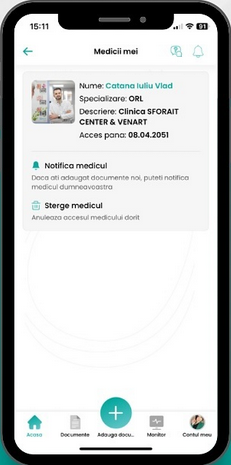
\includegraphics[width=0.35\textwidth]{Medvalet_1.png}} \quad
    \subfloat[Uploaded documents screen]{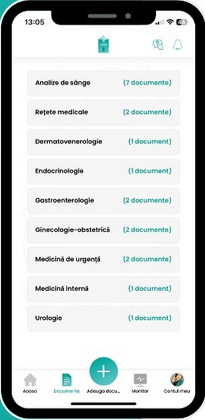
\includegraphics[width=0.35\textwidth]{Medvalet_2.png}}
    \caption{Medvalet screenshots}
    \label{fig:medvalet}
\end{figure}

\begin{table}[h!]
\centering
    \begin{tabular}{|p{0.47\textwidth}|p{0.47\textwidth}|}
    \hline
    \textbf{Key Features/Benefits} & \textbf{Limitations/Drawbacks} \\ \hline
    \begin{itemize}
        \item Upload medical history as PDFs or scanned documents.
        \item Categorize documents by type (e.g., prescriptions, lab results).
        \item Graphically track vitals like blood pressure and weight over time.
        \item Patients can input personal details such as name, age, and weight.
        \item Doctors can access patient history directly via the app.
    \end{itemize} &
    \begin{itemize}
        \item Requires doctors to create accounts, which may deter use.
        \item Doctors can access patient history without explicit consent, raising privacy concerns.
        \item App acts as document storage, which can be cumbersome to access for lengthy histories.
        \item Lacks data extraction or summarization features from uploaded documents.
        \item Only available as a mobile app, limiting accessibility for desktop-only users.
    \end{itemize} \\ \hline
    \end{tabular}
\caption{Medvalet Features and Limitations}
\label{tab:medvalet}
\end{table}

\FloatBarrier

\subsubsection{Andaman7}

A mobile app developed by a Belgian-American eHealth company with the goal to improve doctor-patient communication, compliant with GDPR and HIPAA \parencite{andaman}. See Table \ref{tab:andaman7} for a summary of its features and limitations and figure \ref{fig:andaman7} for a screenshot of the app.

\begin{figure}[ht]
    \centering
    \subfloat[PHR Sections screen]{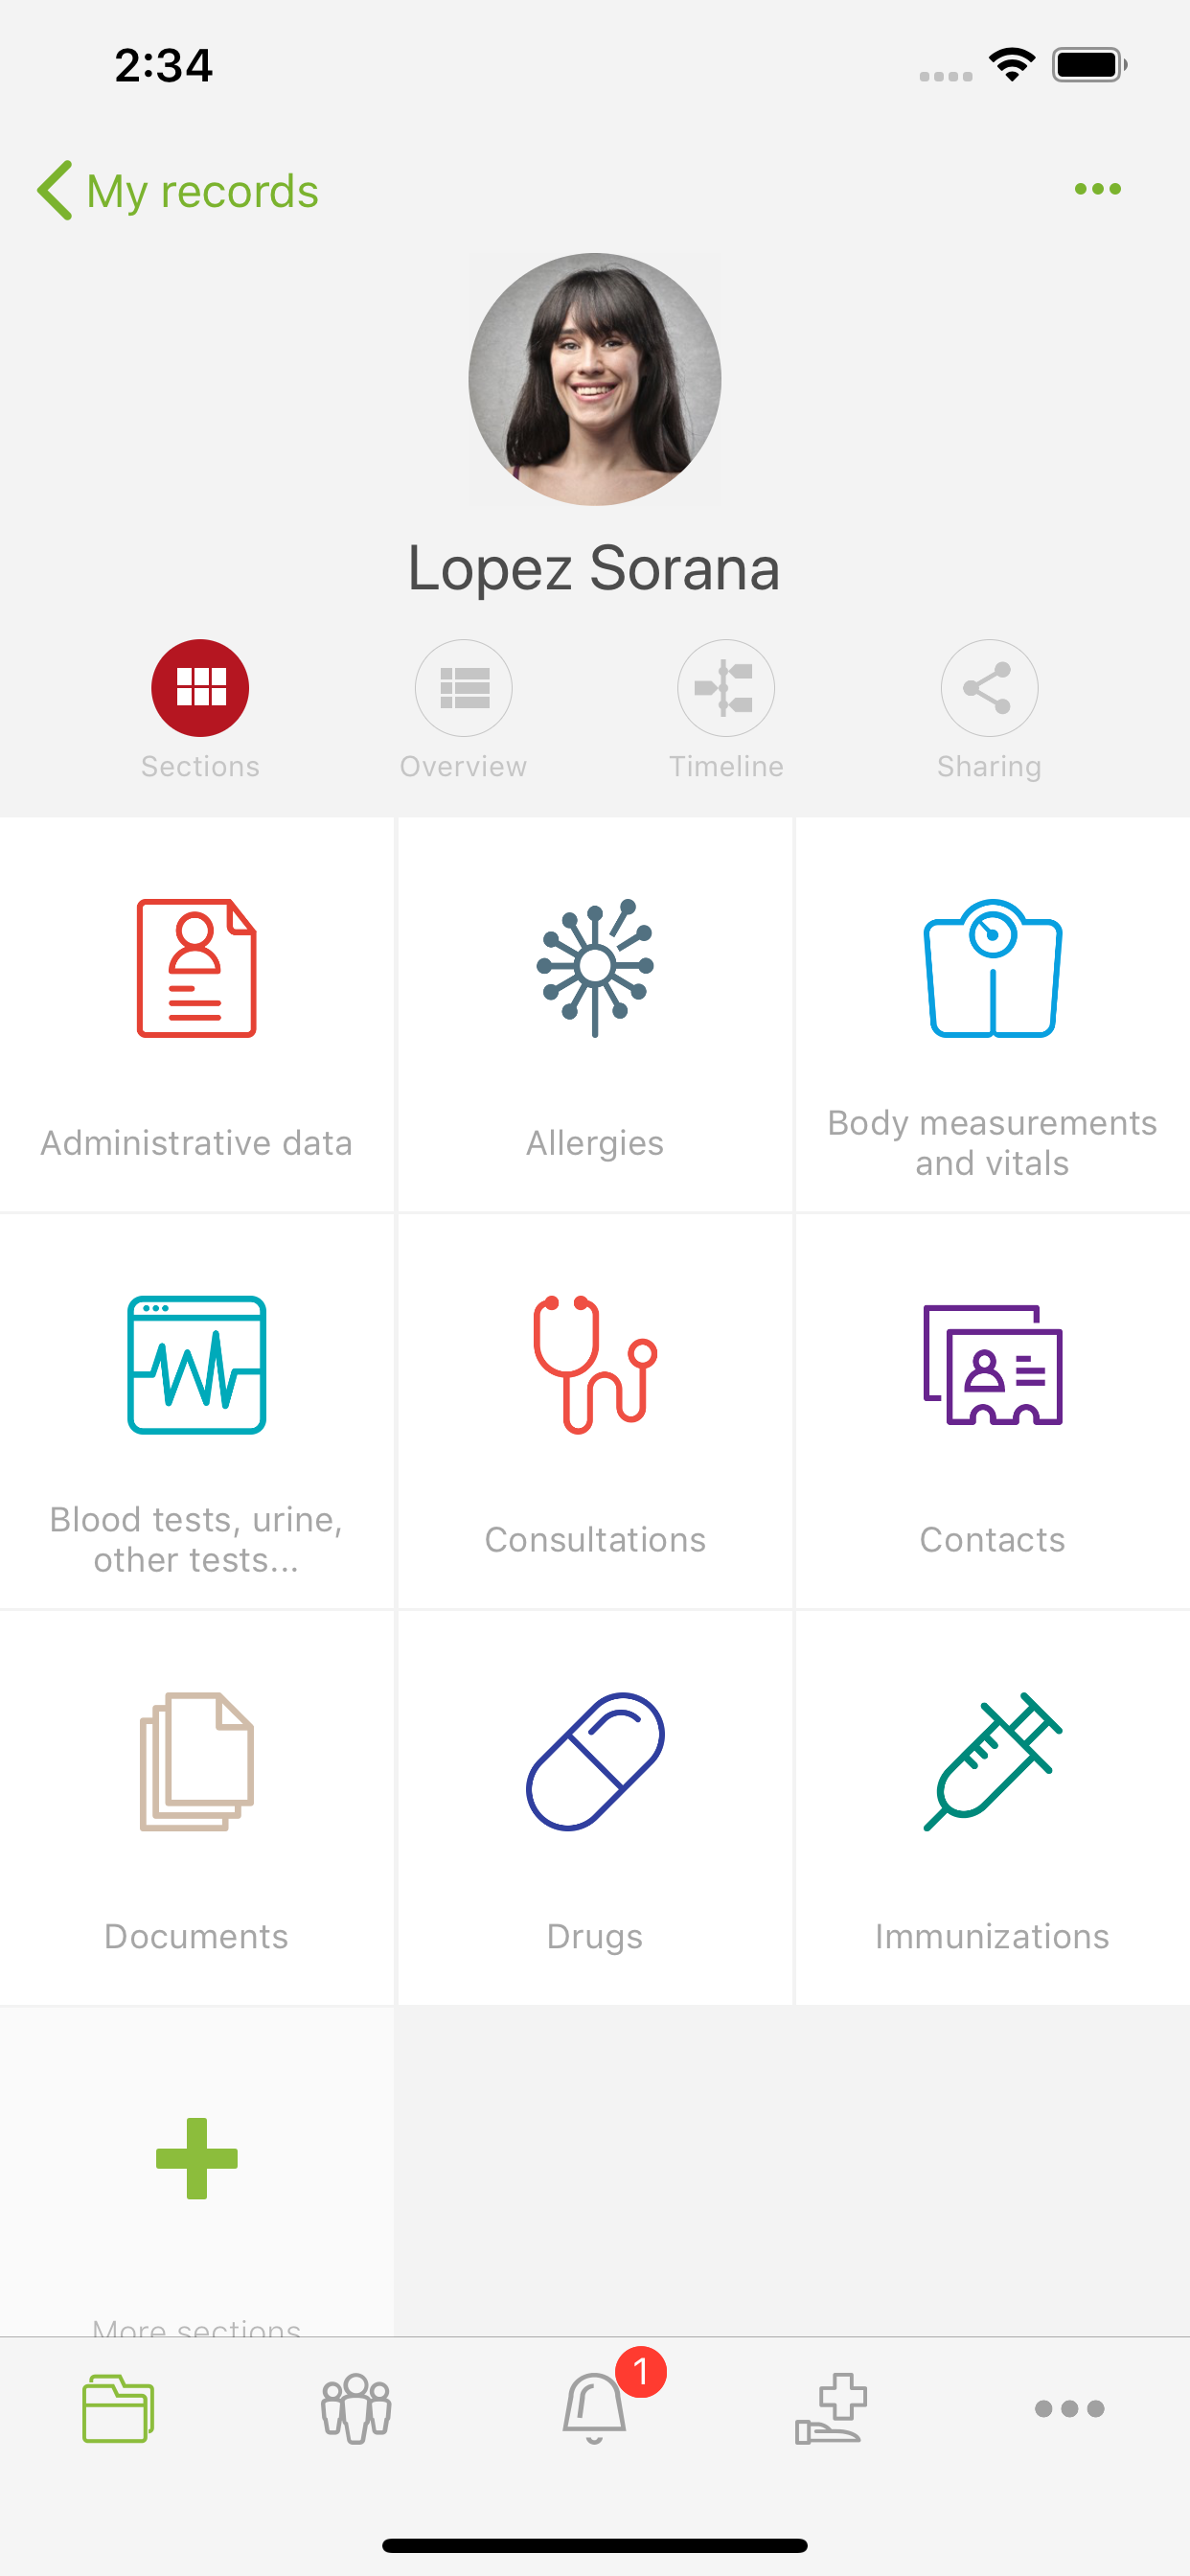
\includegraphics[width=0.45\textwidth]{Andaman_1.png}} \quad
    \subfloat[Documents section screen]{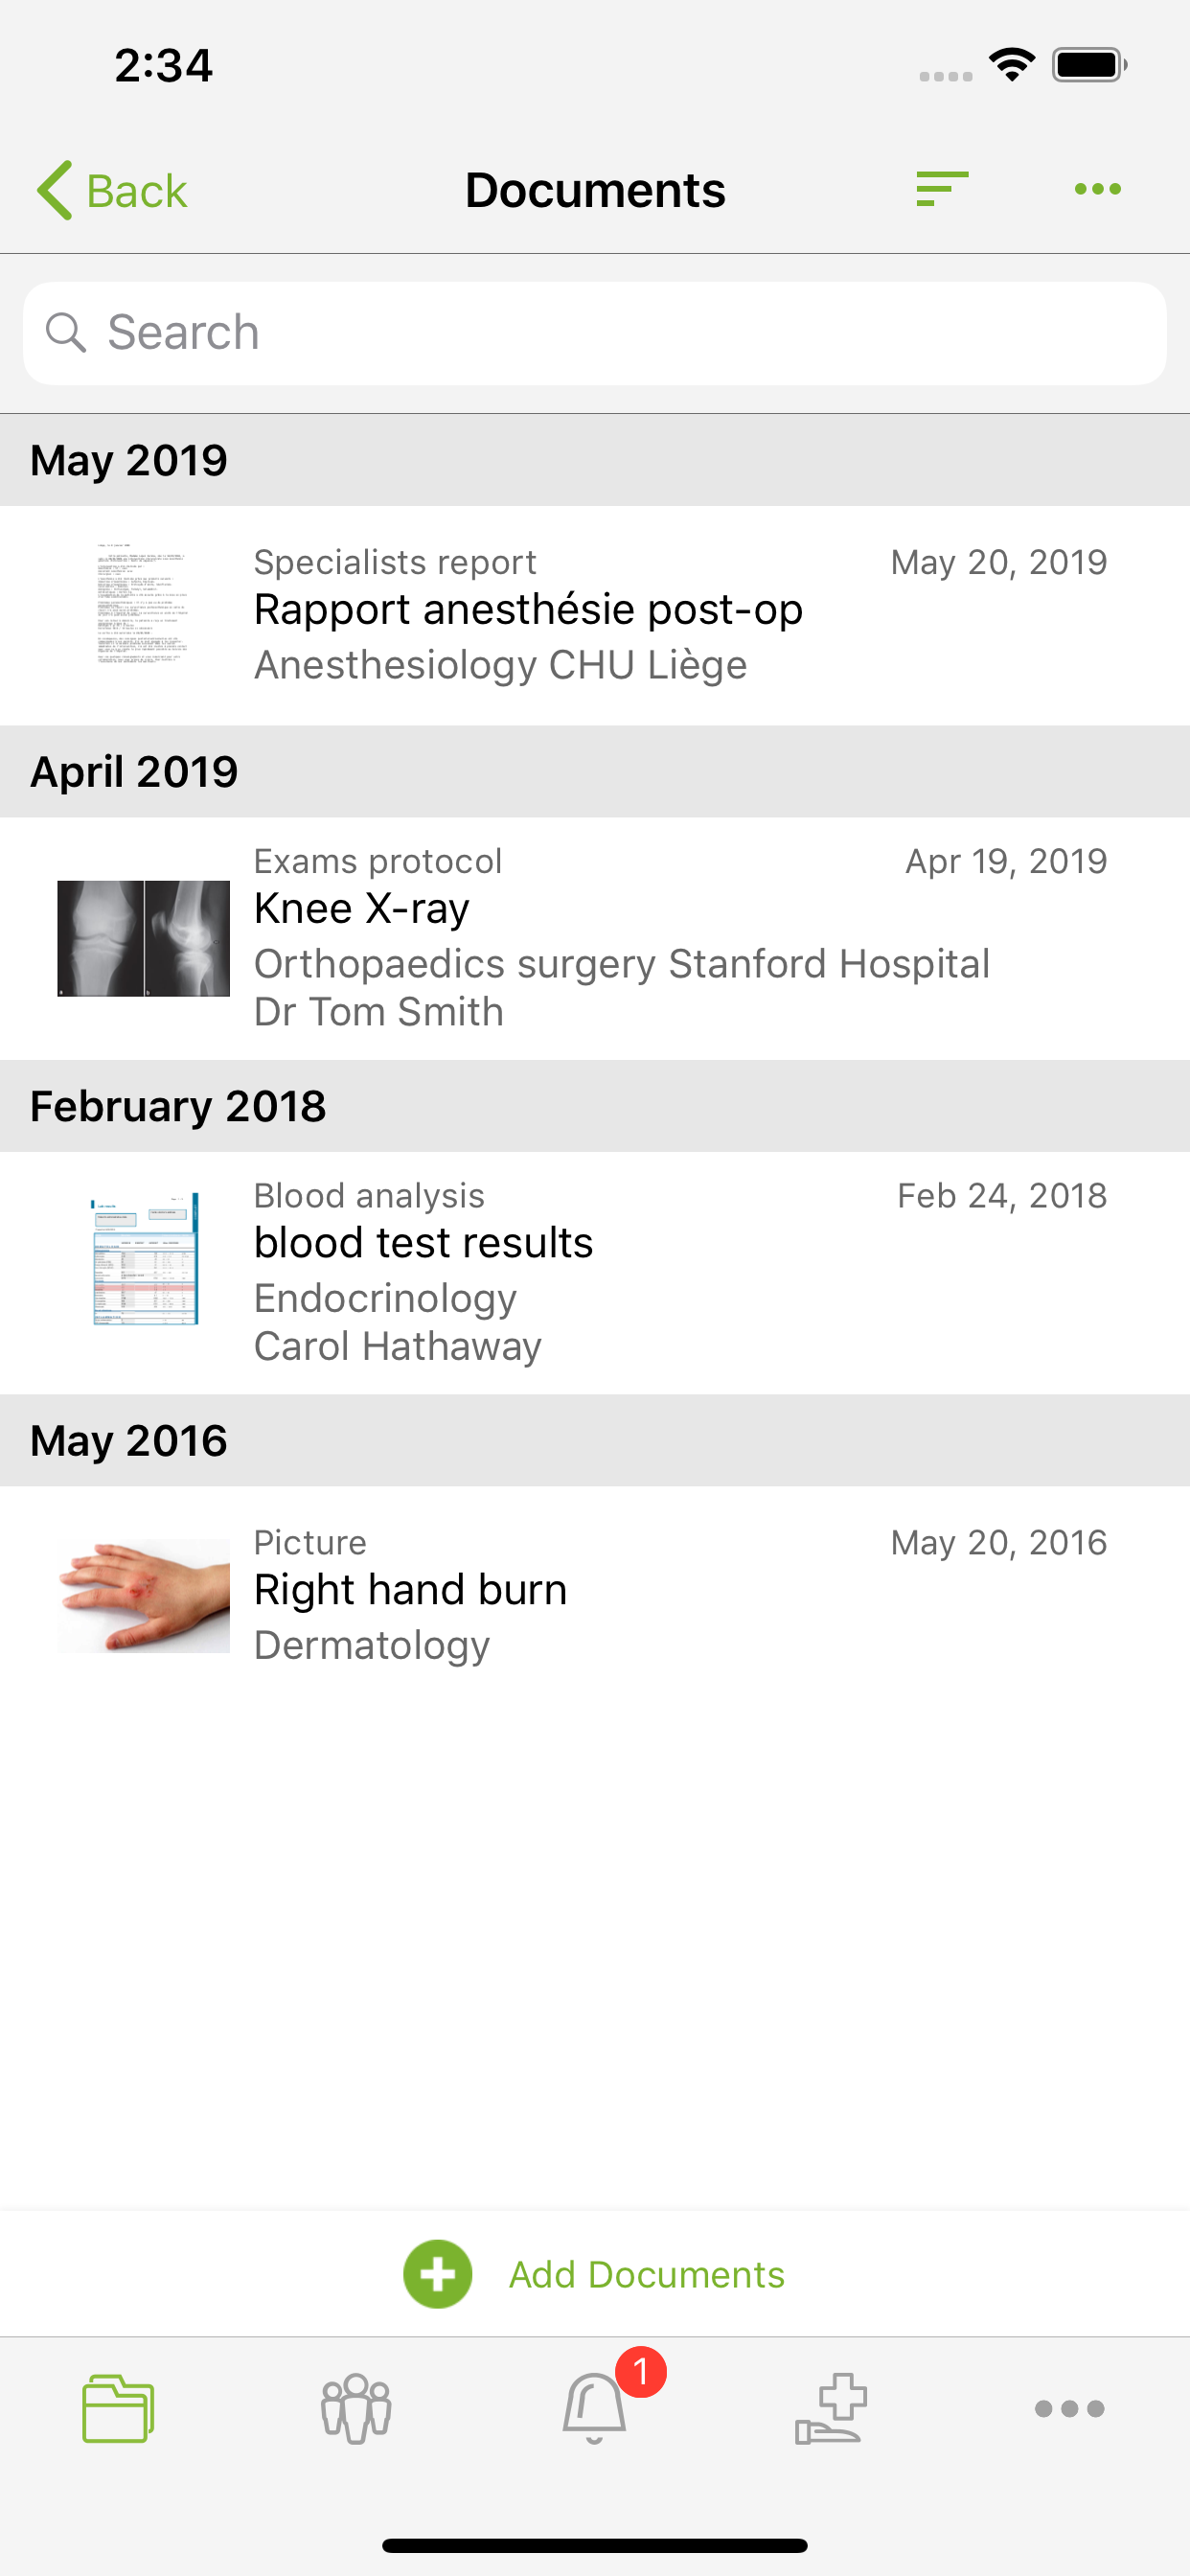
\includegraphics[width=0.45\textwidth]{Andaman_2.png}}
    \caption{Andaman7 screenshots}
    \label{fig:andaman7}
\end{figure}

\begin{table}[htbp]
\centering
    \begin{tabular}{|p{0.47\textwidth}|p{0.47\textwidth}|}
    \hline
    \textbf{Key Features/Benefits} & \textbf{Limitations/Drawbacks} \\ \hline
    \begin{itemize}
        \item Offers sections for personal information, medical history, allergies, vaccinations, medications, etc.
        \item Automatically collects health data from over 300 hospitals and clinics in the US and Europe.
        \item Supports input from diverse sources like hospitals, labs, smart devices or even manual input.
        \item Stores data locally on patients’ devices, ensuring privacy.
        \item Data sharing with QR codes and revokable access.
        \item AI tools for summarization, translation, and simplifying medical jargon.
    \end{itemize} &
    \begin{itemize}
        \item Requires patients and doctors to both create accounts.
        \item Does not extract data or values from uploaded documents like lab results.
        \item Limited to mobile platforms, which may limit usability for desktop-only users.
    \end{itemize} \\ \hline
    \end{tabular}
\caption{Andaman7 Features and Limitations}
\label{tab:andaman7}
\end{table}

\FloatBarrier

\subsubsection{Fasten Health}

An open-source, self-hosted electronic medical record aggregator with optional paid desktop versions for Windows and Mac \parencite{fasten}. See Table \ref{tab:fasten_health} for a summary of its features and limitations and figure \ref{fig:fasten} for a screenshot of the app.

\begin{figure}[ht]
    \centering
    \subfloat[Dashboard screen]{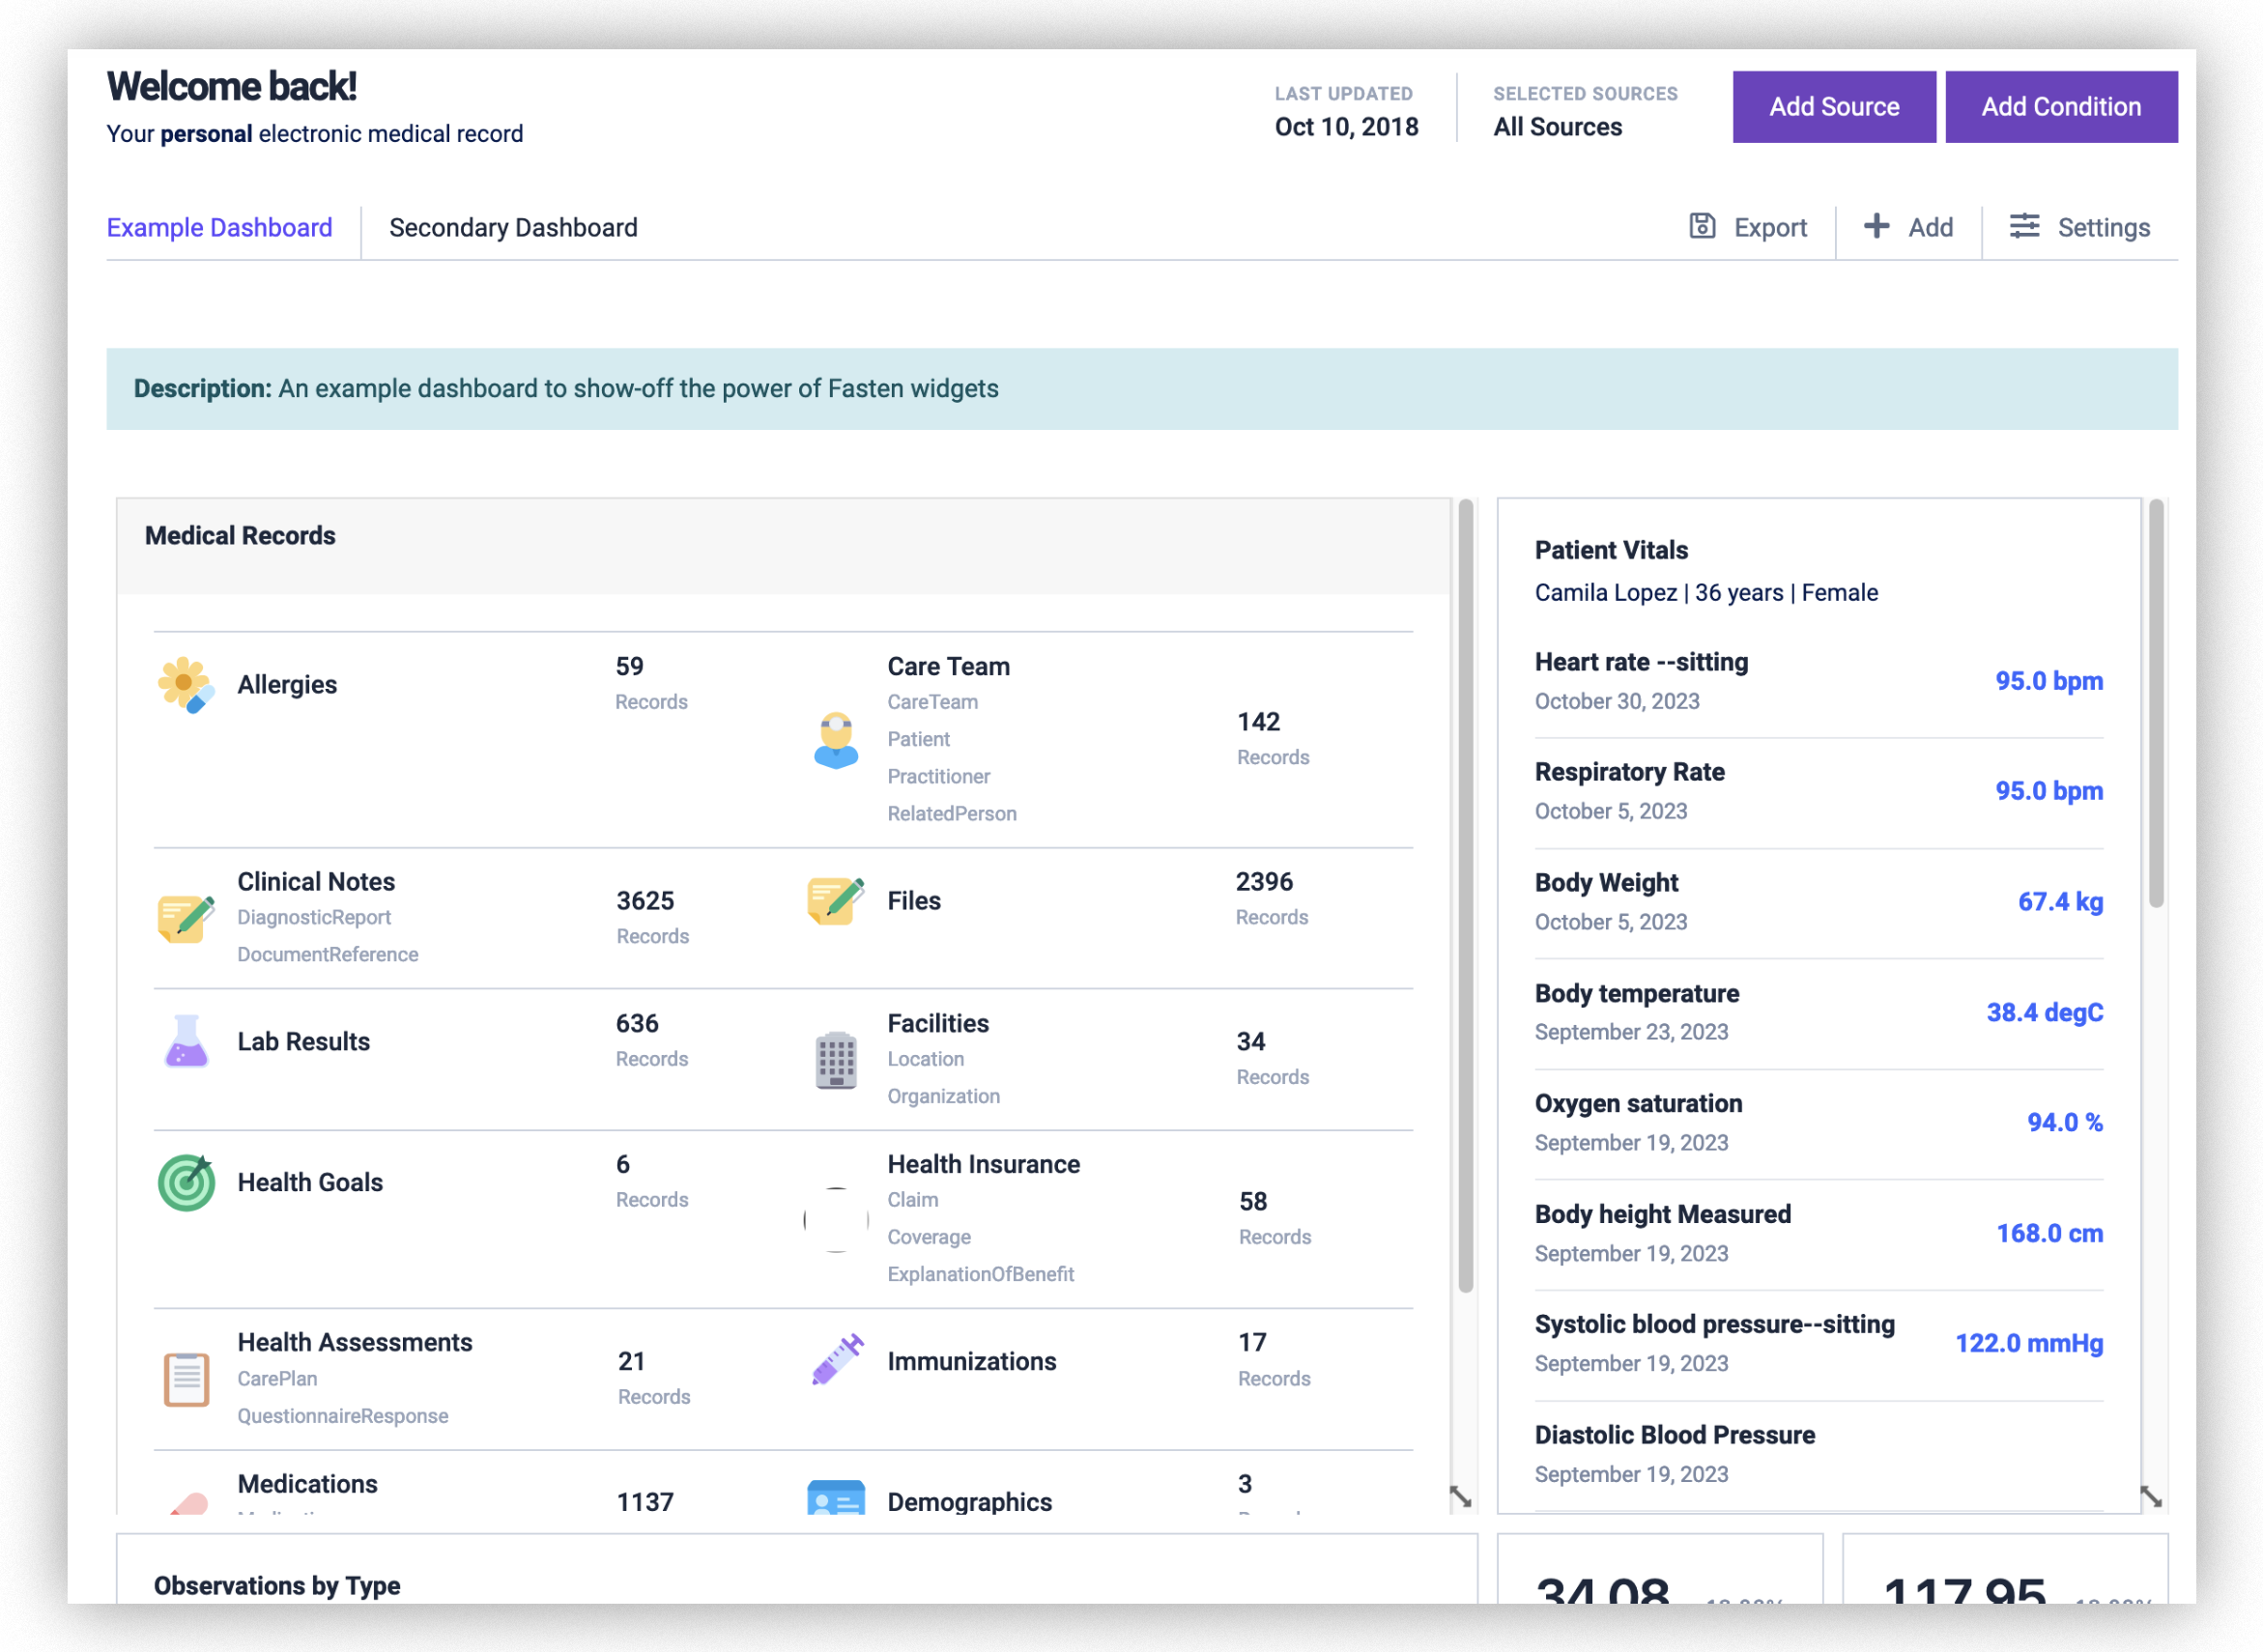
\includegraphics[width=0.75\textwidth]{fasten_1.png}\label{fig:fasten1}} 
    \hspace{0.05\textwidth} 
    \subfloat[Visit history screen]{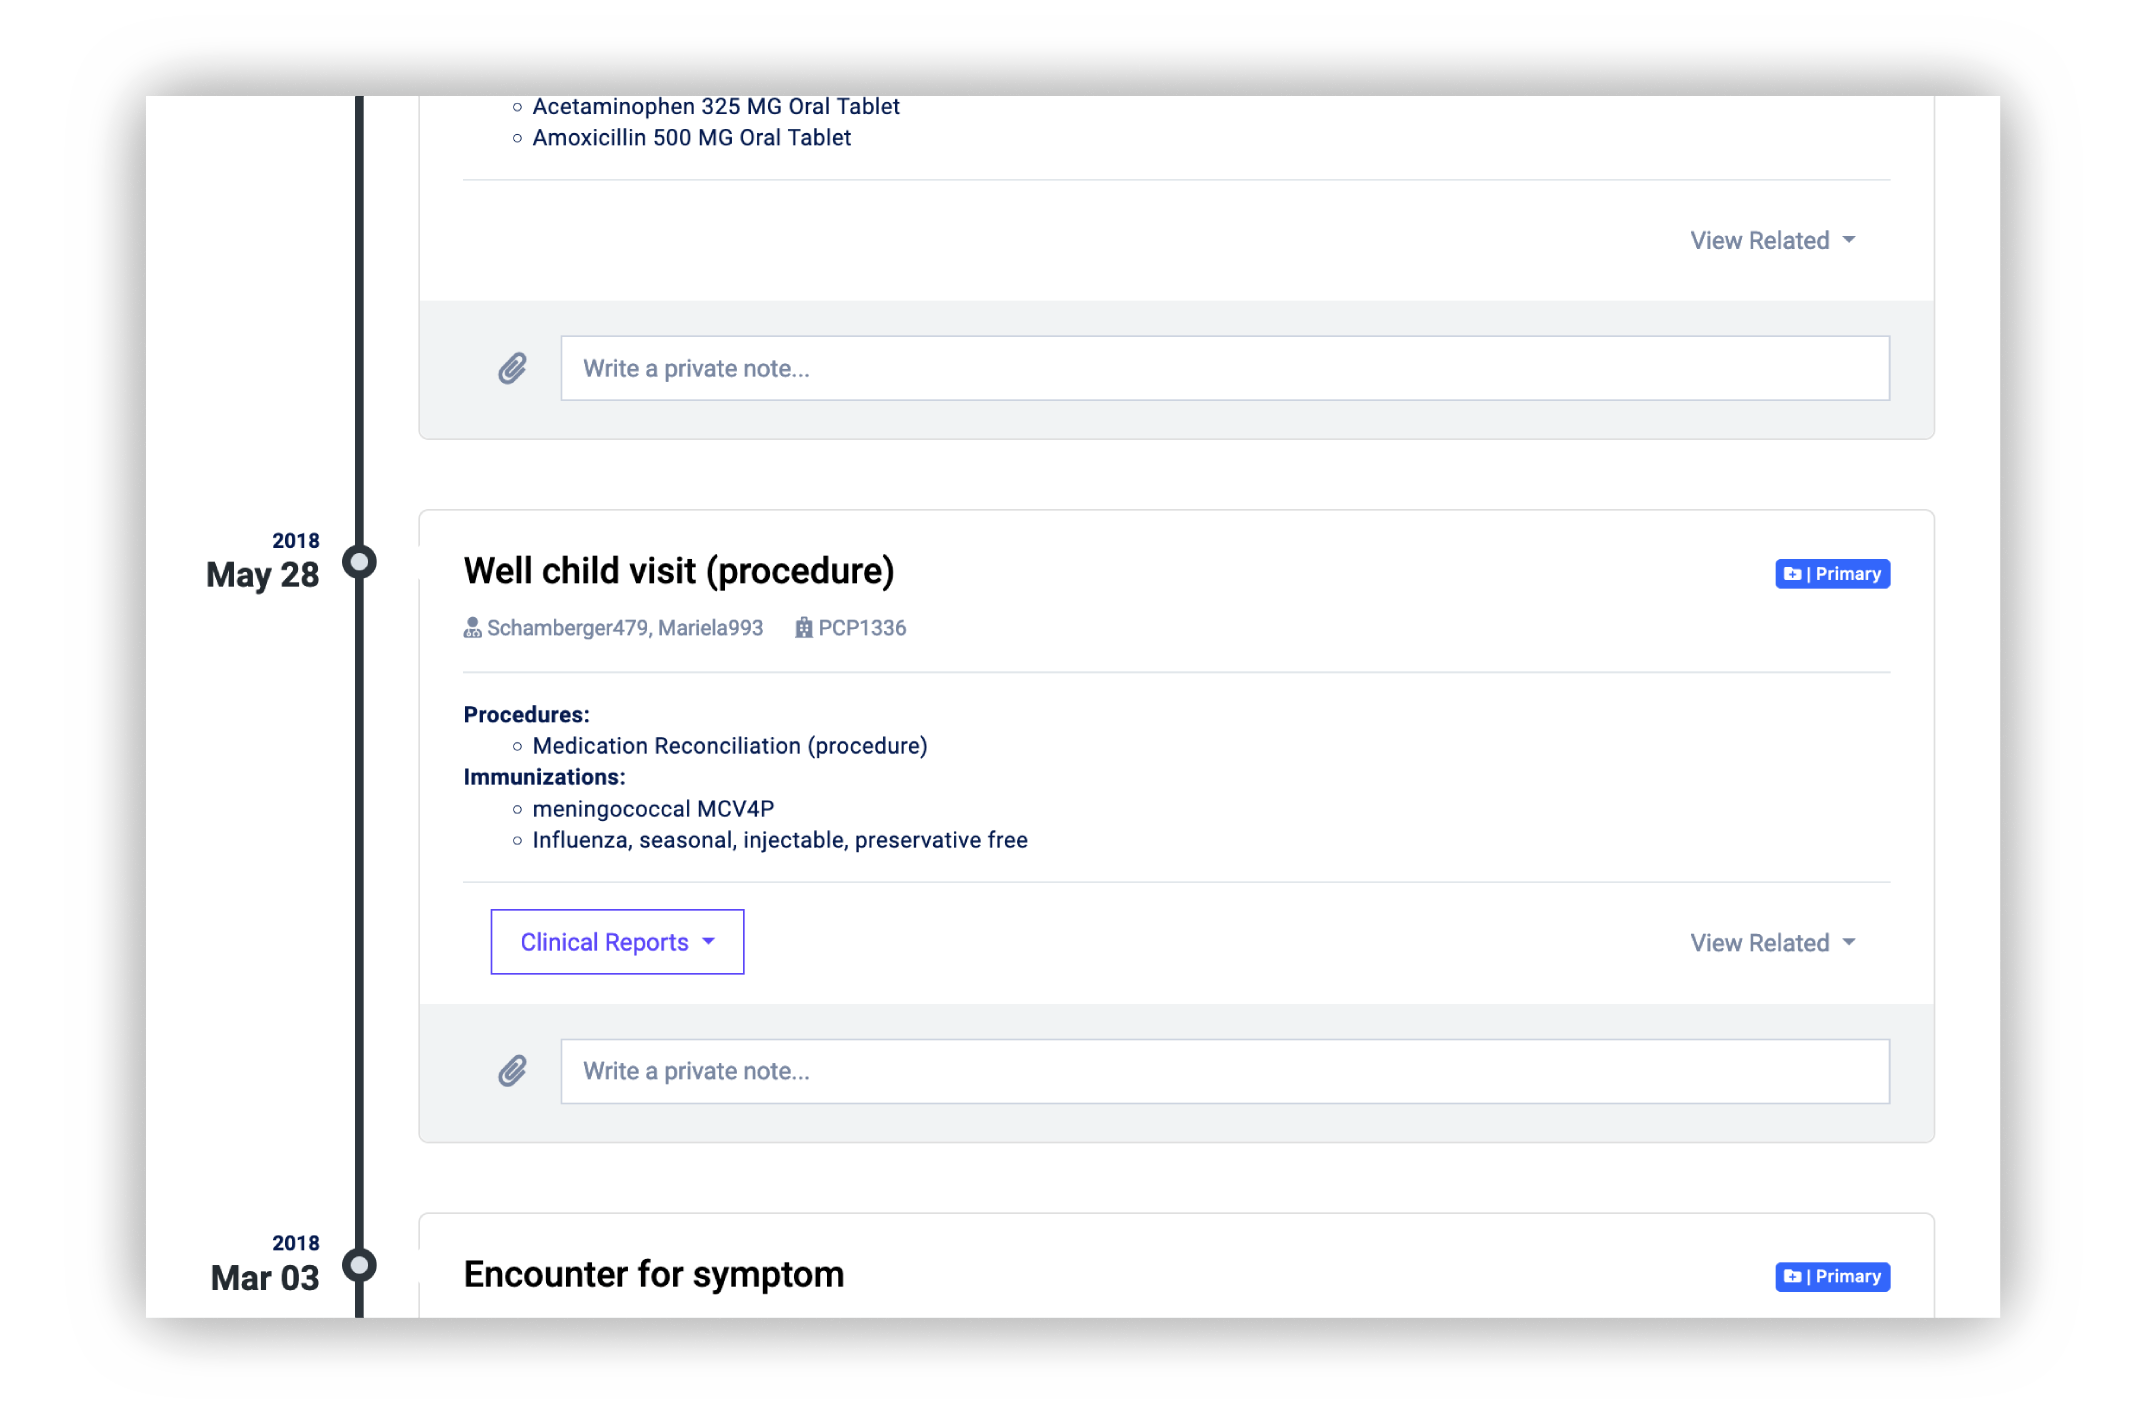
\includegraphics[scale=0.3]{fasten_2.png}\label{fig:fasten2}} 
    \caption{Fasten Health screenshots}
    \label{fig:fasten}
\end{figure}

\begin{table}[h!]
\centering
    \begin{tabular}{|p{0.47\textwidth}|p{0.47\textwidth}|}
    \hline
    \textbf{Key Features/Benefits} & \textbf{Limitations/Drawbacks} \\ \hline
    \begin{itemize}
        \item Automatically aggregates records from multiple providers, like hospitals and labs.
        \item Supports self-hosting for complete control over data, stored locally.
        \item Compatible with protocols such as DICOM, FHIR, and OAuth2.
        \item Allows manual entry for allergies, vaccinations, and medications.
        \item Offers multiple dashboards with graphs to visualize health data.
        \item Supports multi-user functionality for families.
    \end{itemize} &
    \begin{itemize}
        \item Paid desktop versions may deter users.
        \item Manual data entry limited to new or existing encounters, complicating usage.
        \item Does not support OCR or automatic data extraction from documents.
        \item Lacks data-sharing capabilities with doctors.
        \item Requires technical expertise for self-hosting.
        \item Restricted to healthcare providers in the United States.
    \end{itemize} \\ \hline
    \end{tabular}
\caption{Fasten Health Features and Limitations}
\label{tab:fasten_health}
\end{table}


\chapter{Project Planning and Design}

\section{UML Diagrams}

UML, or Unified Modeling Language, is a standardized modeling language that consists of a set of diagrams used for modeling business processes and documenting software systems, helping better communicating potential designs and architectural decisions \parencite{uml}. 

The most common UML diagrams include:
\begin{itemize}
    \item \textbf{Use Case Diagram} - Illustrates the system's intended functionality in terms of actors, use cases, and their relationships, showing how the system delivers value to users. The diagram can also be accompanied by a use case specifications document, which provides a detailed description of each use case.
    \item \textbf{Class Diagram} - Depicts the structure of the system by showing classes, attributes, operations, and static relationships between classes.
    \item \textbf{Sequence Diagram} - Demonstrates how objects interact in a particular, timed sequence scenario, focusing on the messages passed between objects.
    \item \textbf{Activity Diagram} - Represents the workflow of a target use case or business process through a series of activities, emphasizing steps, choices, iterations, and concurrency.
\end{itemize}

The student has used UML diagrams to present the stakeholders with a visual representation of the system's design and functionalities. The diagrams can be found below, under their respective sections.

\subsection{Use Case Diagram}
\begin{figure}[htbp]
    \centering
    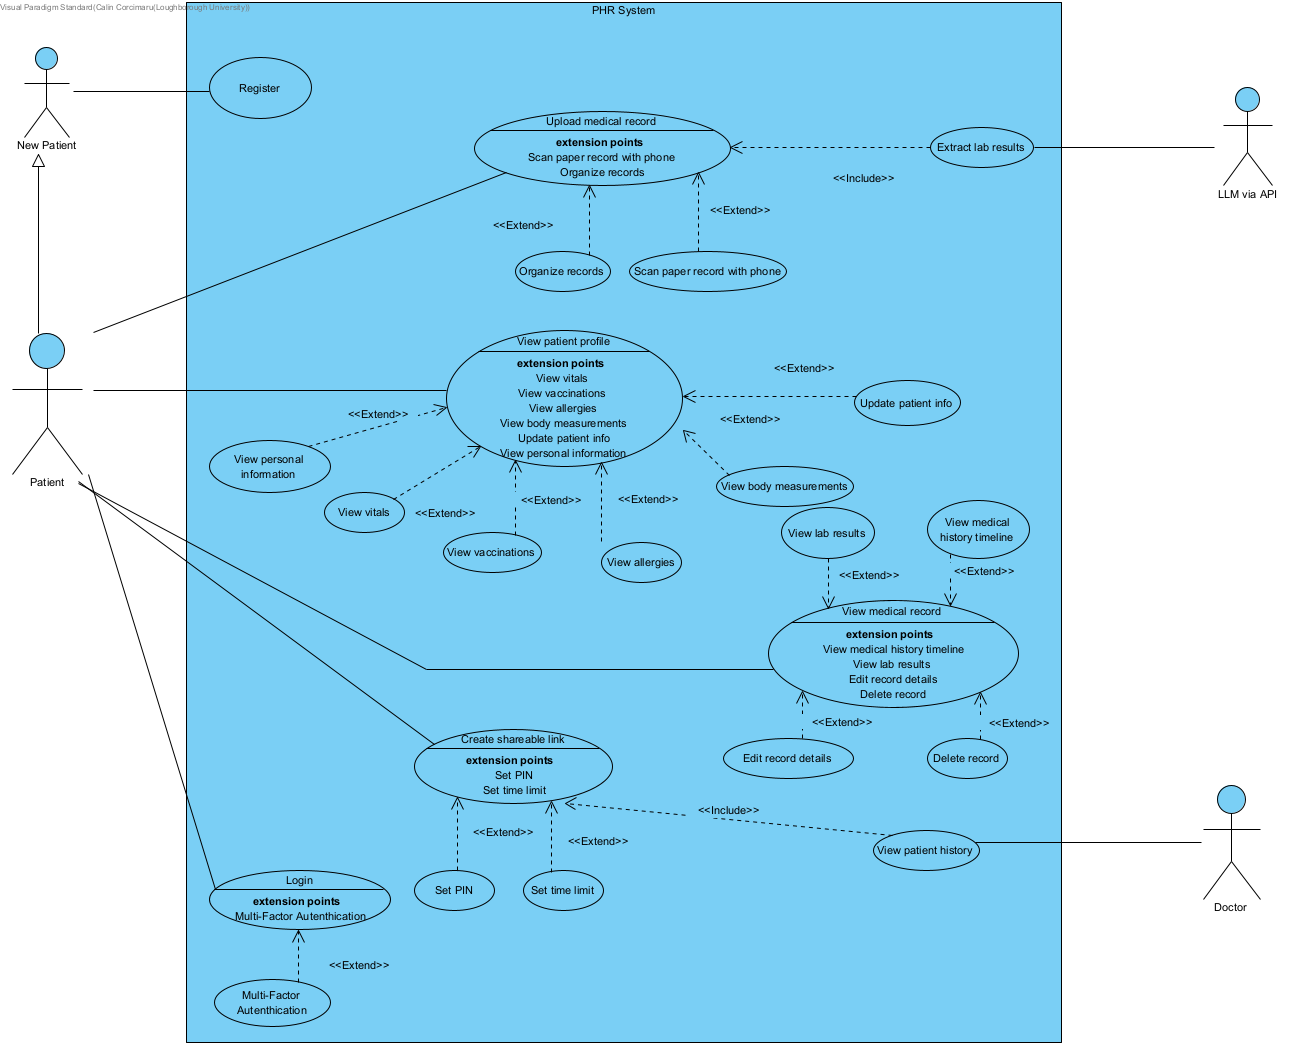
\includegraphics[width=\textwidth,height=0.7\textheight,keepaspectratio]{Use_Case.png}
    \caption{UML Use Case Diagram}
    \label{fig:uml_usecase}
\end{figure}

\FloatBarrier

\subsection{Use Case Specifications}

\subsubsection{Login}
\begin{tabular}{|p{0.2\textwidth}|p{0.7\textwidth}|}
\hline
Description & The Login use case allows the app user to log in to their existing account via their credentials, with an optional use of MFA. \\
\hline
Actors & Patient \\
\hline
Preconditions & Must have an existing account \\
\hline
Steps & 1. User enters user and password \newline
       2. User clicks on the login button \newline
       3. App validates user credentials \newline
       4. Patient enters MFA code if enabled \newline
       5. App logs user in \\
\hline
\end{tabular}

\subsubsection{Register}
\begin{tabular}{|p{0.2\textwidth}|p{0.7\textwidth}|}
\hline
Description & The Register use case allows the app user to create a new account. \\
\hline
Actors & New Patient \\
\hline
Preconditions & No existing account with the email used to register \\
\hline
Steps & 1. User enters user and password \newline
       2. User clicks on the register button \newline
       3. App validates user credentials \newline
       4. App logs user in \newline
       5. App sends verification email \newline
       6. User verifies email \\
\hline
\end{tabular}

\subsubsection{Upload Record}
\begin{tabular}{|p{0.2\textwidth}|p{0.7\textwidth}|}
\hline
Description & The Upload Record use case allows the patient to upload their medical records to the app. \\
\hline
Actors & Patient, LLM \\
\hline
Preconditions & Must be logged in \\
\hline
Steps & 1. User selects file upload (or camera scan) \newline
       2. User selects the record to upload \newline
       3. User clicks on the upload button \newline
       4. App validates the record \newline
       5. User selects the appropriate record type \newline
       6. If record type is lab result, app sends the record to LLM via API for processing into JSON format \newline
       7. App adds the record to the database \newline
       8. App shows confirmation to user \\
\hline
\end{tabular}

\subsubsection{Share Records}
\begin{tabular}{|p{0.2\textwidth}|p{0.7\textwidth}|}
\hline
Description & The Share Records use case allows the patient to share their medical records with doctors. \\
\hline
Actors & Patient, Doctor \\
\hline
Preconditions & Must be logged in and have records uploaded \\
\hline
Steps & 1. User selects option to create a share link \newline
       2. OPTIONAL: User selects the records to share \newline
       3. OPTIONAL: User adds a PIN to the share link \newline
       4. User selects time limit for the share link \newline
       5. App generates the share link \newline
       6. App sends the share link to the doctor via email \newline
       7. App shows confirmation to user \newline
       8. Doctor clicks on the share link \newline
       9. Doctor enters the PIN (if required) \newline
       10. App validates the PIN \newline
       11. App shows the records to the doctor \\
\hline
\end{tabular}

\subsubsection{View Records}
\begin{tabular}{|p{0.2\textwidth}|p{0.7\textwidth}|}
\hline
Description & The View Records use case allows the patient to view and edit their uploaded medical records. \\
\hline
Actors & Patient \\
\hline
Preconditions & Must be logged in and have records uploaded \\
\hline
Steps & 1. App provides a list of records or medical history \newline
       2. User selects record to view from list or medical history \newline
       3. App retrieves the record from the database \newline
       4. App shows the record to the user \newline
       5. OPTIONAL: User can view the record in a graphical format if lab result \newline
       6. OPTIONAL: User edits the record \newline
       7. OPTIONAL: User deletes the record \\
\hline
\end{tabular}

\subsubsection{View Patient Profile}
\begin{tabular}{|p{0.2\textwidth}|p{0.7\textwidth}|}
\hline
Description & The View Patient Profile use case allows the patient to view and edit their profile information, including health information such as allergies, medications, vaccinations and recorded health data like blood pressure, glucose levels, etc. \\
\hline
Actors & Patient \\
\hline
Preconditions & Must be logged in \\
\hline
Steps & 1. User selects the profile section \newline
       2. App retrieves the profile information from the database \newline
       3. App shows the profile information to the user - vaccinations, allergies, medications, health data \newline
       4. OPTIONAL: User edits the profile information \newline
       5. OPTIONAL: User adds new health data \newline
       6. OPTIONAL: User deletes health data \newline
       7. OPTIONAL: User can view health data in a graphical format \\
\hline
\end{tabular}

\FloatBarrier
\clearpage

\subsection{Class Diagram}
\begin{figure}[htbp]
    \centering
    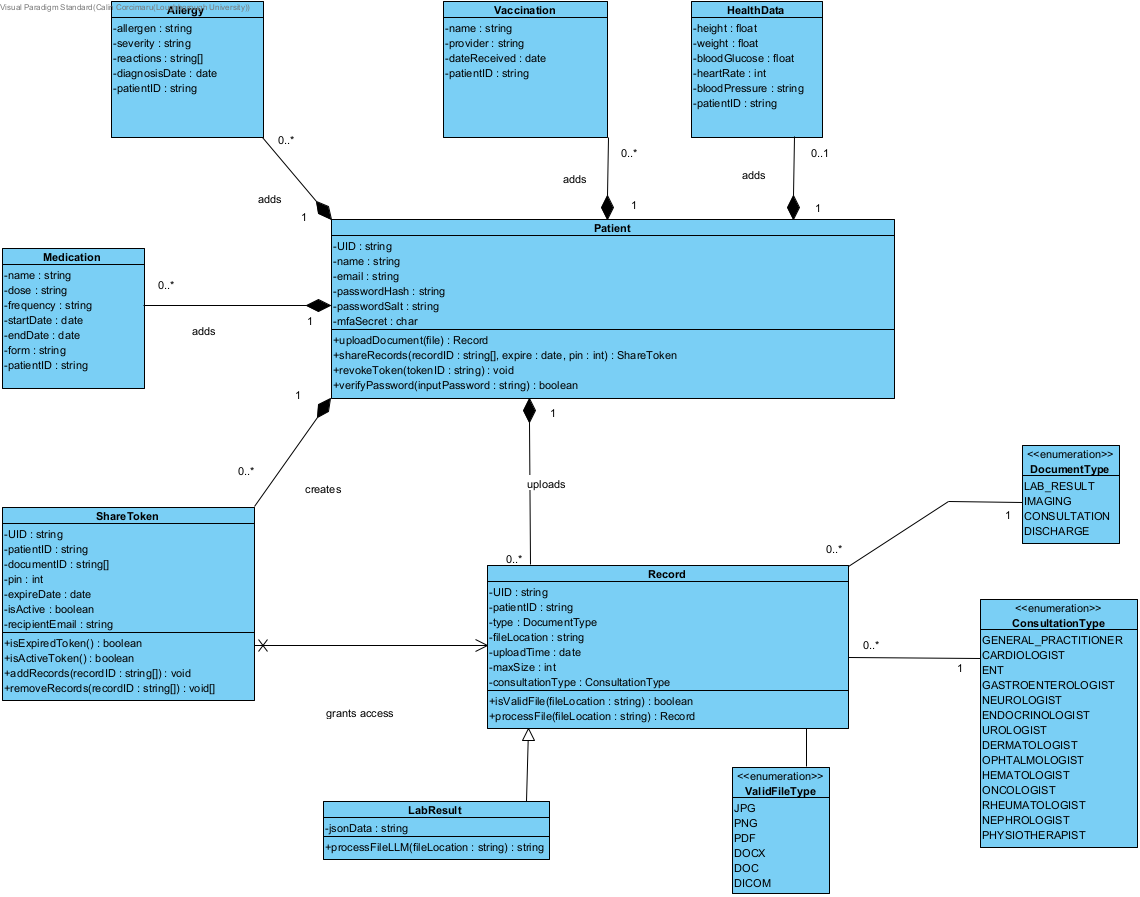
\includegraphics[width=\textwidth,height=0.8\textheight,keepaspectratio]{Class_diagram.png}
    \caption{UML Class Diagram}
    \label{fig:uml_class}
\end{figure}

\FloatBarrier
\clearpage

\subsection{Sequence Diagrams}
\begin{figure}[htbp]
    \centering
    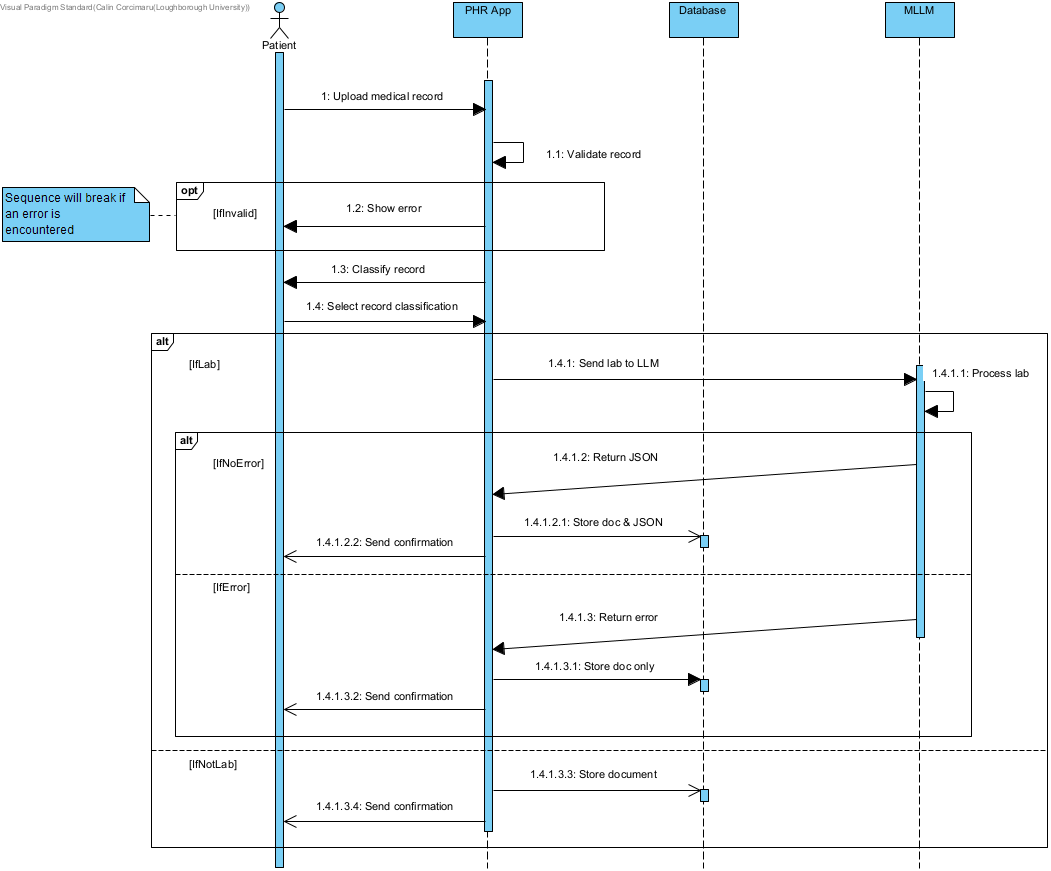
\includegraphics[width=\textwidth,height=0.8\textheight,keepaspectratio]{Sequence_upload.png}
    \caption{UML Sequence Diagram - Upload Record Use Case}
    \label{fig:sequence1}
\end{figure}

\begin{figure}[htbp]
    \centering
    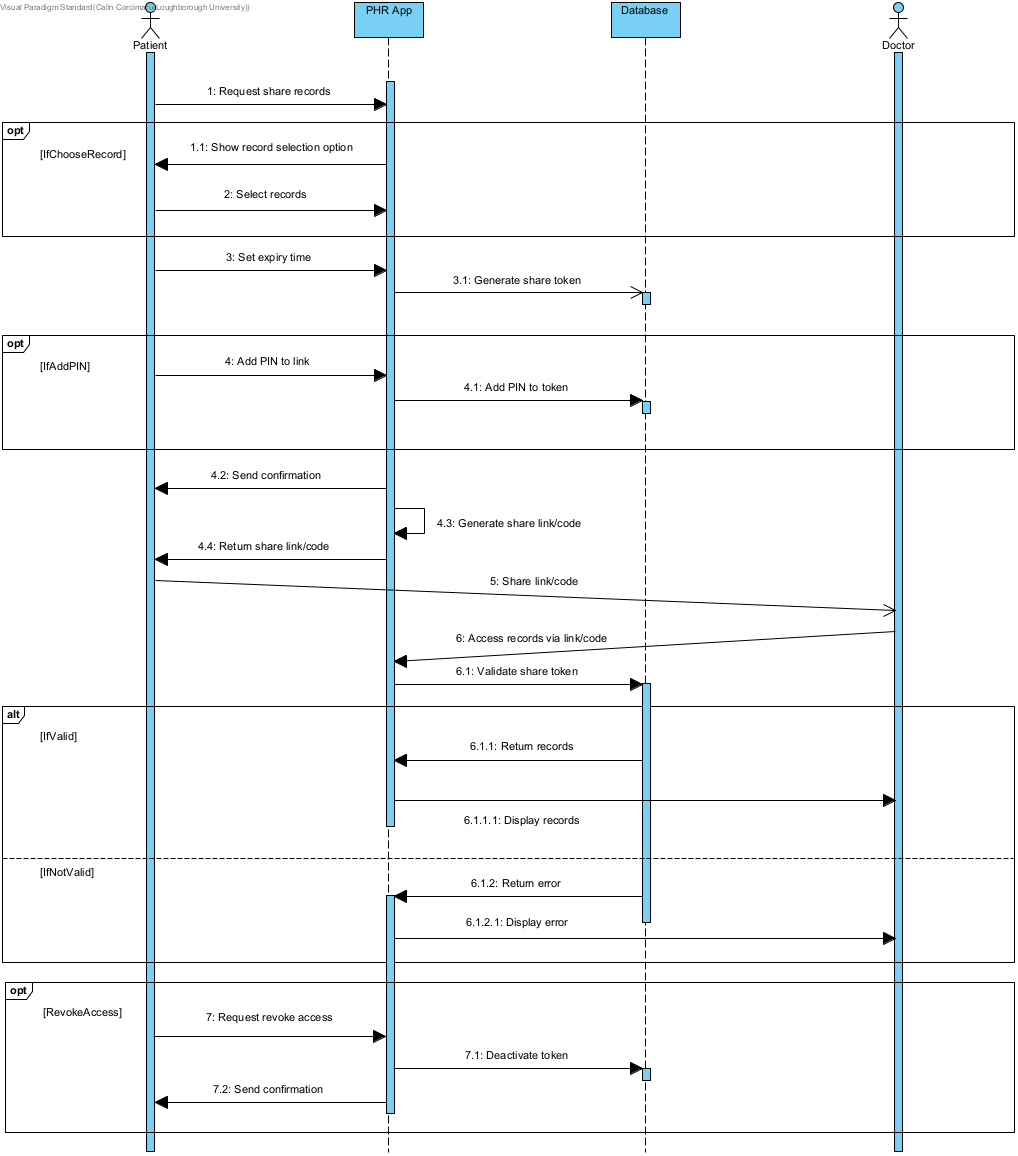
\includegraphics[width=\textwidth,height=0.8\textheight,keepaspectratio]{Sequence_share.png}
    \caption{UML Sequence Diagram - Share Records Use Case}
    \label{fig:sequence2}
\end{figure}

\FloatBarrier

\noindent\begin{minipage}{\textwidth}
    \subsection{Activity Diagrams}
    \begin{center}
        \rotatebox[origin=c]{270}{
            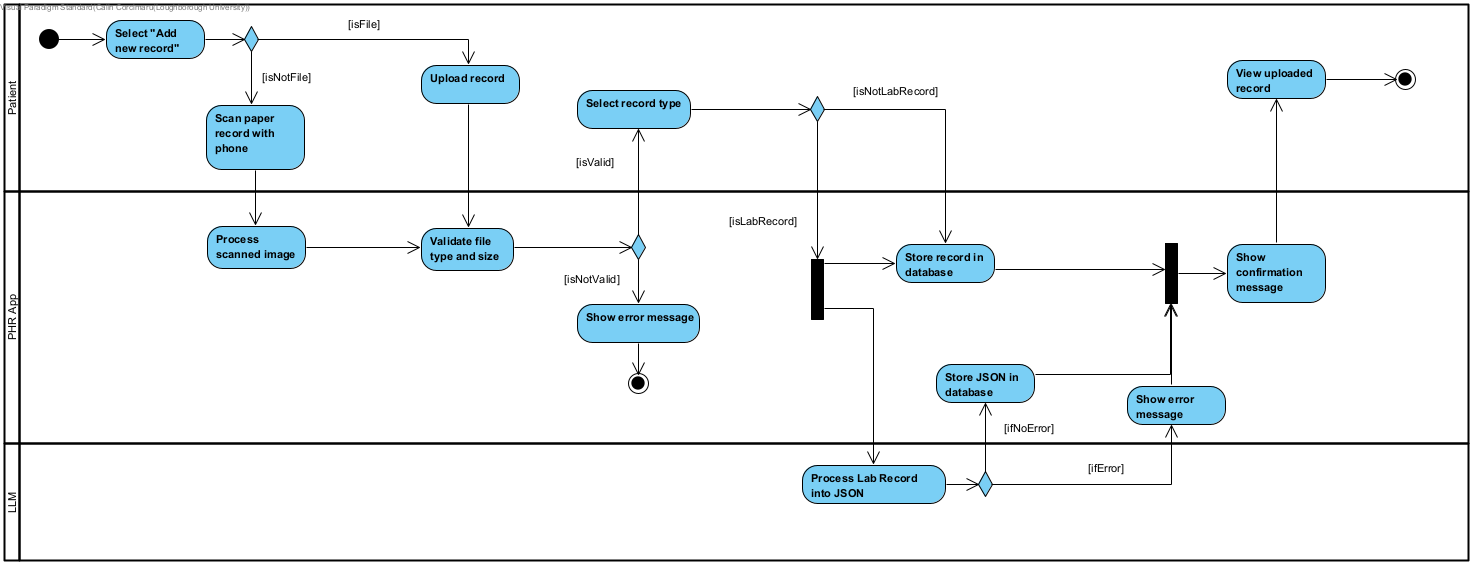
\includegraphics[width=0.9\textheight,keepaspectratio]{Activity_upload.png}
        }
        \captionof{figure}{UML Activity Diagram - Upload Record Use Case}
        \label{fig:activity1}
    \end{center}
\end{minipage}

\noindent\begin{minipage}{\textwidth}
    \begin{center}
        \rotatebox[origin=c]{270}{
            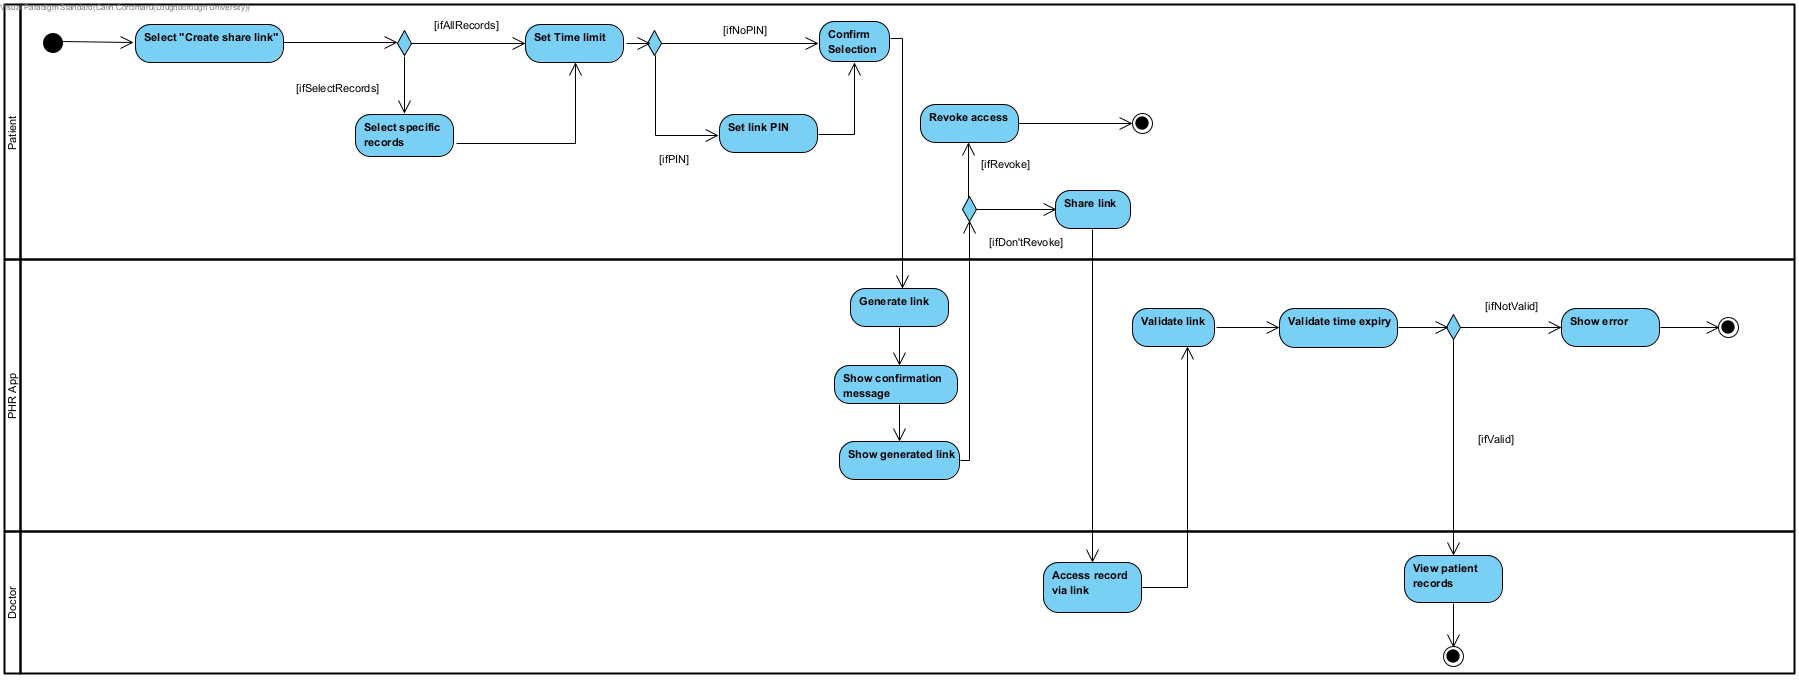
\includegraphics[width=0.9\textheight,keepaspectratio]{Activity_link.png}
        }
        \captionof{figure}{UML Activity Diagram - Share Records Use Case}
        \label{fig:activity2}
    \end{center}
\end{minipage}

\FloatBarrier

\noindent\begin{minipage}{\textwidth}
    \section{Database Design}
    \begin{center}
        \rotatebox[origin=c]{270}{
            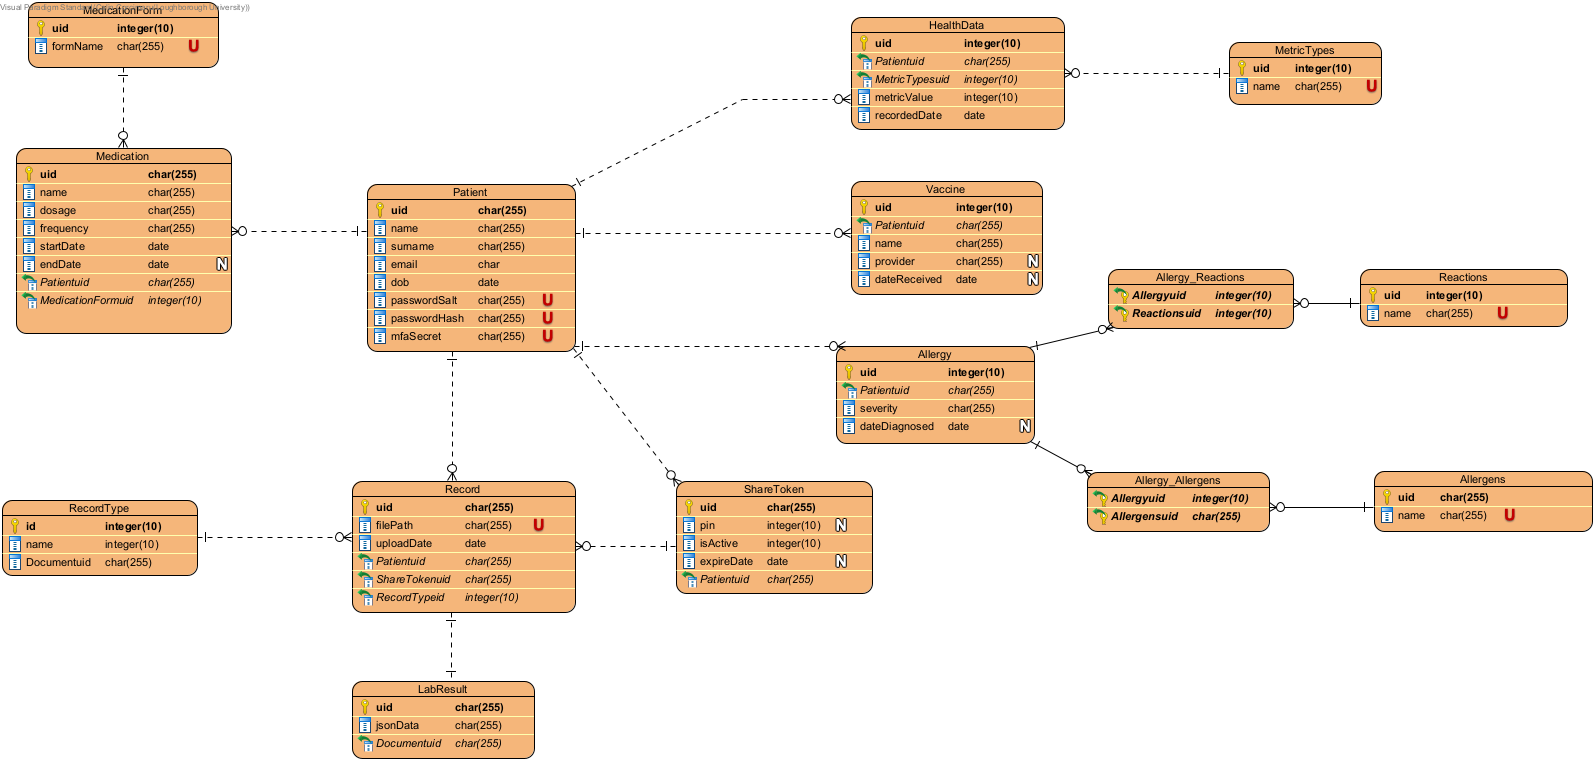
\includegraphics[width=0.9\textheight,keepaspectratio]{ERD.png}
        }
        \captionof{figure}{Entity Relationship Diagram}
        \label{fig:erd}
    \end{center}
\end{minipage}

\FloatBarrier

\section{Wireframes}

\section{Project Tech Stack}

\subsection{Frontend}

\subsection{Backend}

\subsection{Database}

\section{Project Management}

\subsection{Methodology and Tools}

Based on the research above, the student has decided that he will be using a hybrid approach, with Waterfall as the main methodology for planning managing the project. The development part of the project will be done using ScrumBan, so that the student will be able to utilise elements from both frameworks. There are several reasons for this choice:

\begin{enumerate}
    \item The nature of the project - the student is working on a project that has a limited timeframe (about 6-7 months) and is of a smaller scale. 
    \item Documentation requirements - the student is required to document the progress during the project in this report, including the requirements gathered, design considerations and implementation decisions and outcomes. 
    \item Regulatory requirements - the student is required to adhere to the regulations and standards of the healthcare industry, which may require extensive documentation and planning.
    \item Customer involvement - the student will be working closely with the project stakeholder, who will be providing feedback and guidance throughout the project.
    \item Familiarity with both Agile and Waterfall - the student has experience with both Agile (specifically Scrum and Kanban) and Waterfall methodologies, and has worked on projects that have used both approaches.
\end{enumerate}

The student will use Jira Software as their project management tool, which is one of the most popular project management tool for software development projects that supports working with Agile frameworks such as Scrum and Kanban \parencite{atlassian}. The student has experience with Jira Software, having used it in previous projects, and is familiar with its features and capabilities.

\subsection{Project Backlogs}

\subsection{Sprints planning}

\chapter{Development}

This chapter will discuss the development of the project. Rather than going into detail how each sprint has been done, it will focus on the main features implemented, how this was achieved and will talk about successes or challenged that were encountered in the development process.

\section{Sprint \#1}

The first sprint of this project was focused in laying the groundwork for the project, which mainly involved setting up the schemas for the ORM that would create the tables for the database, the initial setup of the API endpoints, such as the login and register endpoints, authentication and other security measures, but also setting up the frontend of the project.

\subsection{SQLModel Schemas \& Database creation}

SQLModel played a pivotal role in helping quickly build the database tables. As previously mentioned in~\ref{sec:techstack}, SQLModel is built on top of SQLAlchemy and Pydantic, both being very powerful Python libraries. Pydantic was used to create the schemas that were used both within the backend but also by SQLAlchemy to create the tables in the database. 

Below is an example of a schema that was used to create the User table in the database.

\begin{lstlisting}[language=Python, caption=SQLModel User Schema]
# Base model that contains the field serialiser for date formatting to dd-mm-yyyy and the date field itself
    class DateFormattingModel(SQLModel):
        dob: date | None = None
    
        @field_serialiser('dob')
        def serialise_dob(self, value: date) -> str:
            return value.strftime("%d-%m-%Y")
    
    class User(DateFormattingModel, table=True):
        id: uuid.UUID = Field(default_factory=uuid.uuid4, primary_key=True)
        name: str
        email: EmailStr = Field(index=True, unique=True)
        hashed_password: str
\end{lstlisting}

Similarly, SQLModel (and more specifically Pydantic schemas) could be used to create response/request models that would be used by the endpoints to validate the data that was being sent to or by the API. These schemas did not create tables in the database, but were used to control or validate the data being sent to or from the API.

Below is an example of a SQLModel/Pydantic schema that was used to validate the data that was being sent to the register endpoint.

\begin{lstlisting}[language=Python, caption=SQLModel Auth Schema]
    # User Data model used for login and registration
    class UserAuth(SQLModel):
        email: EmailStr
        password: str
        name: str | None = None # Will only be used for registration

    # User Data model used for most API responses
    class UserPublic(SQLModel):
        id: uuid.UUID
\end{lstlisting}

\subsection{Authentication \& APIs}

As the project was centered around building a PHR system that would deal with sensitive health data, one of the main concerns was the security of the system and its users. 

One of the important choices to make was how to handle the authentication. Based on research on modern authentication methods, the student has identified 4 different ways to handle authentication in the project:

\begin{itemize}
    \item JWT Tokens
    \item OAuth2
    \item Session-based authentication
    \item Using 3rd party authentication services, like Auth0
\end{itemize}

Each method has its own disadvantages and advantages, which will be briefly discussed below.
JWT (JSON Web Tokens) authentication involves generating tokens containing user information for client-side storage \parencite{auth1}. While it requires minimal server-side management, tokens can be vulnerable to XSS and CSRF attacks and cannot be invalidated once created \parencite{auth1, auth2}. The authors recommend using methods like pairs of access and refresh tokens to mitigate these risks, and also to store the tokens in cookies.

Session-based authentication stores session information server-side, using cookies to maintain client sessions \parencite{auth1, auth2}. While cookies can face similar security risks as JWT, they can be secured through flags like HttpOnly and SameSite \parencite{mozilla}. Sessions can be invalidated server-side, providing better security control.

Third-party authentication options include OAuth2 through providers like Google \parencite{auth2, auth3} or services like Auth0 \parencite{auth0}. While these offer quick implementation, they may introduce dependencies or security concerns due to third-party data storage. 

Moldova's electronic government iniatives have created MPass, which is a national Single Sign On (SSO) authentication system that offers a secure and easy way to access electronic government services \parencite{mpass}. While it may not be possible to currently integrate MPass into the system, it will be considered as a possible future integration, given the system's Moldovan user focus, which will be discussed in the~\ref{sec:future_work} section.

In the end, the student decided to go with a session-based authentication system. One of the main reasons was its ease of implementation that still provided a good level of security. The ability to control the session on the server side was an additional, important factor that contributed to this decision. This allows the system to safely log out users, invalidate sessions due to inactivity or suspicious activity, and also to control the session's lifetime, all without relying on storing tokens on the client side.

Sessions were created in the backend by storing them in a Session table in the database. The table contained a Session ID, which was passed to the user as a cookie. Upon a succesful login, the backend would set the cookie in the user's browser, which would then be sent with every request to the server. 

To ensure that the cookies were safe from common attacks like Cross-Site Scripting (XSS) and Cross-Site Request Forgery (CSRF), the student security used guidance from \cite{owasp,mozilla} to set the following flags on the cookies:

\begin{lstlisting}[language=Python, caption=Session Cookie Flags]
    # Set the session cookie in the response and send it to the client
    response.set_cookie(
        "session_id",
        str(session_id), # Using str() to convert the UUID to a string
        httponly=True,
        max_age=3600, # 1 hour
        samesite="strict",
        secure=True)
\end{lstlisting}

To further secure the system, some of the endpoints that were created in this sprint were protected by using session validation checks to ensure that the user was authenticated before accessing the endpoint. This was achieved thanks to FastAPI's dependency injection system, which allowed the student to create a dependency that would check if the user was authenticated before allowing the request to continue. An example of this can be seen below:

\begin{lstlisting}[language=Python, caption=FastAPI Dependency for Session Validation]
@app.post("/logout")
async def logout(
  response: Response, 
  request: Request, 
  user_id: uuid.UUID = Depends(validate_session), 
  session: Session = Depends(get_session)
):
  session_id = request.cookies.get("session_id")
  cookie_user_id = session.get(AuthSession, uuid.UUID(session_id)).user_id
  
  if cookie_user_id != user_id:
    raise HTTPException(
      status_code=403, 
      detail="You do not have permission to log out this user"
    )
  
  # Code that deletes session and the cookie
  return {"status": status.HTTP_200_OK, "message": "Logout successful"}

async def validate_session(request: Request, session: Session = Depends(get_session)):
  session_id = request.cookies.get("session_id")
  if not session_id:
    raise HTTPException(
      status_code=status.HTTP_401_UNAUTHORIZED, 
      detail="Session cookie not found"
    )
    
  existingAuthSession = session.exec(
    select(AuthSession)
    .where(AuthSession.id == uuid.UUID(session_id))
    .where(AuthSession.expires_at > datetime.now())
  ).first()
    
  if not existingAuthSession:
    raise HTTPException(
      status_code=status.HTTP_401_UNAUTHORIZED, 
      detail="Session not found"
    )
    
  return existingAuthSession.user_id
\end{lstlisting}

Finally, to ensure that the system was secure, the system also used a hashing algorithm to hash the passwords before storing them in the database. The student identified multiple hashing algorithms that could be used, with the main contenders being bcrypt, scrypt and Argon2. 

Bcrypt is a popular and secure hashing algorithm that is widely used in the industry \parencite{hash3, hash2}. It is considered to offer an optimal balance between security and speed, making it a popular choice for real-world implementation \parencite{hash1}. In 2 of the previously mentioned papers, bcrypt was ranked on the mid-to-high end of the security scale, with algorithms such as scrypt and Argon2id being scored higher in the dimension of security \parencite{hash1, hash3}. The authors of these papers concluded that Argon2id was the best choice for hashing passwords, followed closely by scrypt and bcrypt. However, while scrypt and Argon2id are more secure, they are also more computationally expensive, and may require more configuration to be used effectively \parencite{hash1}.

In the end, the decision was made to use bcrypt as the hashing algorithm. The main reasons for the use of this algorithm was its simplicity of use, wide adoption and its balance between security and perfomance. The passlib library was used to hash the passwords before storing them in the database. The library allowed for automatic salt generation and storage within the hash and by default, it used a work factor of 12, which is considered to be a good balance between security and performance. An example of this can be seen below:

\begin{lstlisting}[language=Python, caption=Hashing passwords with bcrypt]
    # Util function to verify the password hash against the plaintext password
    def verify_hash(plaintext_password: str, hashed_password: str) -> bool:
        return bcrypt.verify(plaintext_password, hashed_password)
    
    # Util function to create a password hash from the plaintext password
    def create_hash(plaintext_password: str) -> str:
        return bcrypt.hash(plaintext_password)
\end{lstlisting}

A final security measure that could've been implemented was a rate limiter to all of the created endpoints. Similarly, Starlette, the framework FastAPI was built on top of, also offered other middleware such as HTTPSRedirectMiddleware, TrustedHostMiddleware, and others that could be used to further secure the system. However, in the interest of time, it was decided to leave these for a future sprint.

\subsection{Frontend Setup}

While most of the work done in this sprint was done in the backend, some work was also done in the frontend, mainly focusing on the login and register pages. Here, the student used the PrimeVue component library to quickly and easily create the forms that would be used to log in and register users.

An example of PrimeVue components being used can be seen below in the Register page. Some of the components taken from PrimeVue include InputText, DatePicker, Password, Button and Message. 

\begin{lstlisting}[language=HTML, caption=PrimeVue components in the Register page]
          <DatePicker
            name="dob"
            dateFormat="dd/mm/yy"
            placeholder="Data nasterii"
            showIcon
            fluid
            :maxDate="maxDate" />
\end{lstlisting}

\begin{figure}[htbp]
  \centering
  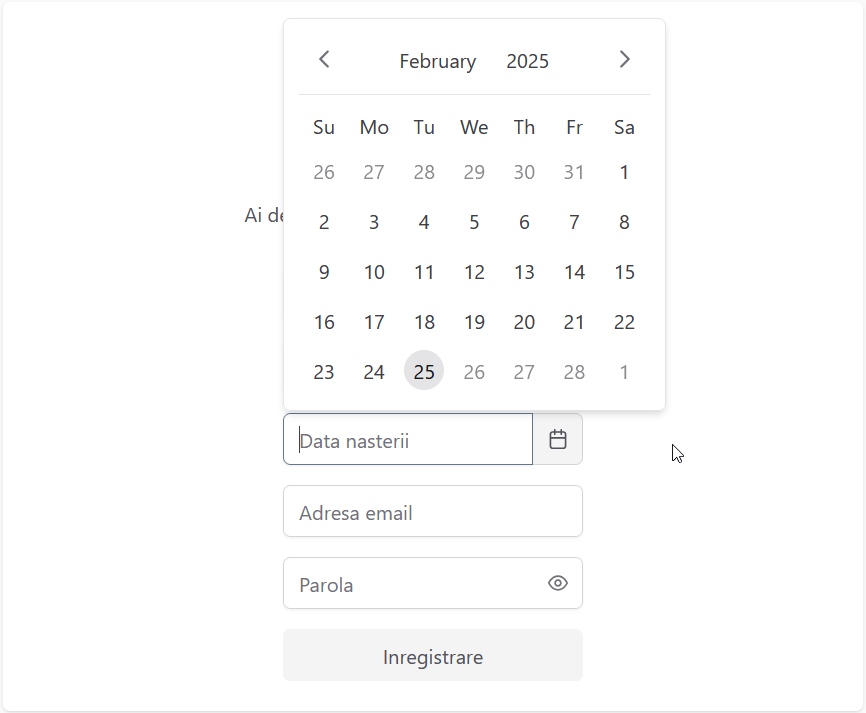
\includegraphics[width=\textwidth,height=0.8\textheight,keepaspectratio]{DatePicker.png}
  \caption{PrimeVue DatePicker component}\label{fig:datepicker}
\end{figure}

\FloatBarrier{}

As previously mentioned in~\ref{sec:techstack}, Vue also comes with other in-built tools that help create a well-working frontend. One of these tools is Vue Router, which was used to create the routes for the frontend. The student created a simple router that would allow the user to navigate between different pages. A navigation guard was used to protect the routes that required the user to be authenticated. An example of this can be seen below:

\begin{lstlisting}[caption=Vue Router Navigation Guard]
router.beforeEach(async (to) => {
  const authStore = useAuthStore()

  if (to.meta.requiresAuth) {
    await authStore.checkAuth() // Check if user is authenticated for protected routes
    if (!authStore.isAuthenticated) {
      return { name: 'Login' } // Redirect to login if not authenticated
    }
  } 
  // More code to handle other cases
})
export default router
\end{lstlisting}

Similarly, Pinia store was used to manage the authentication state of the user in the frontend. The store was then used by elements like the Navigation Guard to check if the user was authenticated before allowing them to access certain routes. An example of the store can be seen below:

\begin{lstlisting}[caption=Pinia Store for Authentication]
export const useAuthStore = defineStore('auth', () => {
  const isAuthenticated = ref(false)
  const user = ref(null)

  async function checkAuth() { // check if user is authenticated
    try {
      const response = await api.get('/me') // return user object if user is authenticated
      isAuthenticated.value = true // user is authenticated
      user.value = response.data.user
    }
    // More code to handle errors and no authentication
  }
  return { isAuthenticated, user, checkAuth }})
\end{lstlisting}

\subsection{Challenges}

\subsubsection{Lack of experience}

One of the biggest challenges encountered in this sprint was the lack of experience using some of the frameworks and libraries used in the project. As such, this sprint's progress moved slower due to the learning curve that needed to be overcome first by reading the documentation and finding any guides/help online.

\subsubsection{System-related decisions}

Another challenge was making decisions regarding different sections of the system, such as authentication, hashing algorithms, and others. Additional time was spent researching the best practices for each respective functionality \- analysing their advantages, disadvantages and ways to implement them in the current system.

\subsection{Requirements completed}

As this was the first sprint, the main focus was on setting up the groundwork for the project. The main requirements completed in this sprint were:

\begin{itemize}
    \item The system must provide a secure login mechanism for patients by using a combination of login and password.
    \item The database must store the user credentials in a secure manner.
    \item The system must be accessible on all modern desktop and mobile-based browsers.
    \item The system must allow patients to add their own personal information, such as name or date of birth.
    % TODO: Add more requirements
\end{itemize}

\section{Sprint \#2}

The second sprint of this project was focused on building some of the smaller elements of the system, such as the ability to add vaccines, allergies and medications. The decision to start with the smaller elements was made to allow the student to get a better understanding of how the frameworks used in the project worked and to get a better understanding of how to structure the project.

\subsection{Adding Vaccines, Allergies and Medications functionality}

The student started by creating the schemas for the Vaccines, Allergies and Medications tables in the database. These tables were created in a similar way to the User table, using SQLModel schemas. Afterwards, the student created the endpoints that would allow the user to add, update, delete and view the data in these tables.

On the frontend side, the system used Vue's main strengths to enable a smooth developer and future user experience. Some of the strengths used were using Vue components to create reusable elemenets, such as a Vaccine Card that would be used to display the vaccines that the user had added. The card also used other Vue elements such as props and emits to pass data between parent and child elements and pass events, respectively. An example of the Vaccine Card can be seen below:

\clearpage

\begin{lstlisting}[language=HTML, caption=Vue Vaccine Card Component Example]
<Card class="w-full" :pt="cardStyles">
  <template #title>
    <span class="font-bold text-2xl">{{ name }}</span>
  </template>
  <template #subtitle>
    <div class="flex items-center justify-between">
      <div>
        <span class="font-bold">{{ provider }}</span>
        <span>{{ date_received }}</span> 
      </div>
      <div>
        <Button icon="pi pi-eye" class="p-button-rounded p-button-text"
          @click="emit('showFile', props.id)" v-if="hasCertificate"/>
        <Button icon="pi pi-ellipsis-h" class="p-button-rounded p-button-text"
          @click="toggle"/>
        <Menu ref="menu" :model="items" :popup="true" />
      </div>
    </div>
  </template>
</Card>  
\end{lstlisting}

The VaccineCard component can then be easily used in the main view:

\begin{lstlisting}[language=HTML, caption=Using VaccineCard Component]
<VaccineCard
  v-for="vaccine in vaccines"
  :key="vaccine.id" 
  v-bind="vaccine"
  :has-certificate="!!vaccine.certificate"
  @delete="deleteVaccine"
  @open-edit="openEditDialog"
  @show-file="showCertificate"
/>
\end{lstlisting}

\begin{figure}[htbp]
  \centering
  
\includegraphics[width=\textwidth,height=0.7\textheight,keepaspectratio]{VaccineCard.png}
  \caption{Vue Vaccine Card component}\label{fig:vaccinecard}
\end{figure}

\FloatBarrier{}

This format was used across the system to easily create reusable components that could be used in multiple places, making the system more modular and easier to maintain.

To make sure the data displayed in the frontend was always up to date, the frontend used Vue's reactivity system. This allowed the data to be automatically updated whenever any change was made to the data in the backend or frontend. Examples of the reactivity system in use can be seen below, with functions that add and delete vaccines from the frontend when called:


\begin{lstlisting}[language=HTML, caption=Vue Reactivity System]
// Will add a vaccine to the vaccines array, which will automatically 
// create a new VaccineCard element
const addVaccine = (vaccine) => {
  vaccines.value.push(vaccine)
}

// Will remove a vaccine from the vaccines array, which will 
// automatically remove the VaccineCard element
const deleteVaccine = (id) => {
  vaccines.value = vaccines.value.filter((vaccine) => vaccine.id !== id)
}
\end{lstlisting}

\subsection{File Uploads}

Another major feature that was implemented in the 2nd sprint was the ability to upload files. At the time of implementation, the feature was only to be used for uploading vaccine certificates, however it could be easily extended to other parts of the system, such as uploading health records or lab results.

To allow a proper upload of files, a new table was created in the database, called FileUpload. This table contained the file metadata, such as its name, size, type, path and others. Similarly, a new table for Allergy Severity was created to ensure consistency in the user uploads and to allow for easy filtering and searching of the data.

The updated ERD diagram with the new tables can be seen below in figure~\ref{fig:erd_s2}:

\noindent\begin{minipage}{\textwidth}
  \begin{center}
      \rotatebox[origin=c]{270}{
          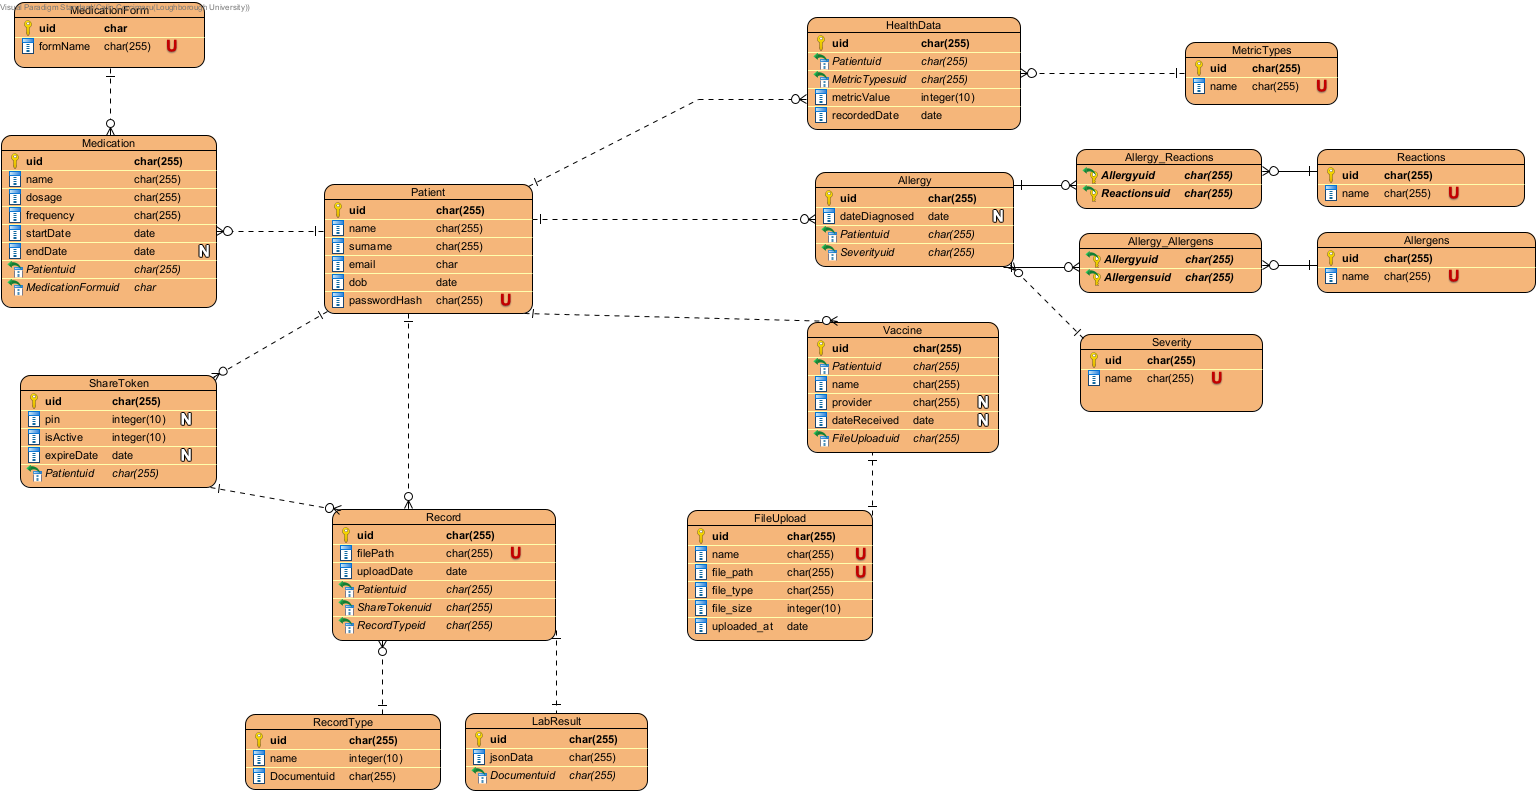
\includegraphics[width=0.95\textheight,keepaspectratio]{ERD_updatedS2.png}
      }
      \captionof{figure}{Updated Entity Relationship Diagram \- Sprint \# 2}\label{fig:erd_s2}
  \end{center}
\end{minipage}

To add more security to the system, the files were further encrypted before being stored in the database. AES was chosen as the encryption algorithm. Based on the articles analysed, it was consistently found to have the best balance between security and performance among other symmetric and asymmetric encryption algorithms \parencite{crypt1,crypt2,crypt3}. The choice to go with a symmetric algorithm was made due to its simplicity, as the key could be stored on the server-side in an environment variable, allowing the encryption and decryption of the files to be done on the server-side. This also allowed to avoid the issue of users losing access to their files if they lost their private encryption key, in the case of asymmetric encryption.

The encryption was done using the Fernet symmetric encryption algorithm from the cryptography library. Fernet uses AES-128 to encrypt the files. The key used to encrypt the files was stored in the environment variables and was generated when the system was started. In the interest of time, no rotation system for the key was implemented, however this would be a good feature to add in the future. 

The file upload process can be seen in figure~\ref{fig:fileuploadview} below. The file upload process was done in two steps. The first step was to upload the file to the server by using multipart form data. The next step would have the file be validated by checking its file type and size, then encrypted and stored in the file system and database. To access the files, the system used a new endpoint that would allow the user to download the file. The endpoint would take the file ID as a parameter and would stream the file to the user.

\begin{figure}[htbp]
  \centering
  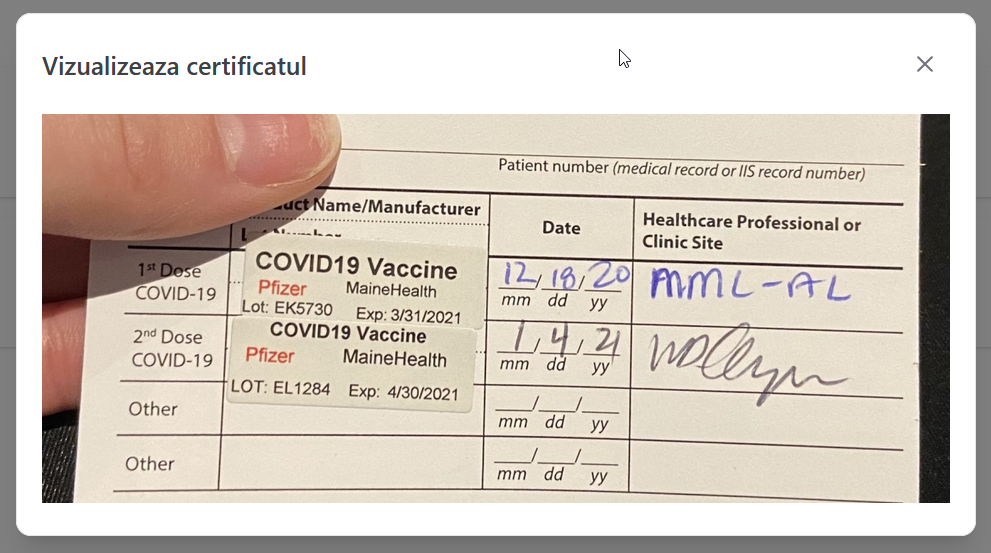
\includegraphics[width=\textwidth,height=0.7\textheight,keepaspectratio]{VaccineCertificate.png}
  \caption{Uploaded Vaccine Certificate}\label{fig:vaccinecertificate}
\end{figure}

\FloatBarrier{}

\begin{figure}[ht]
  \centering
  \subfloat[File Upload Sequence Diagram]{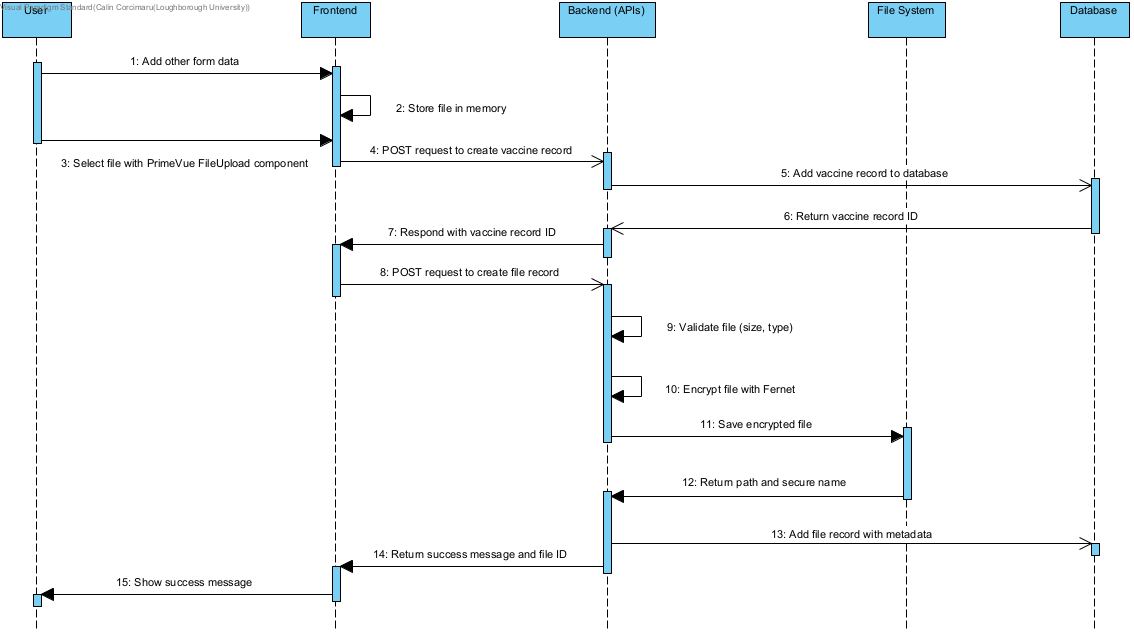
\includegraphics[width=\textwidth]{Sequence_FileUpload.png}\label{fig:seqfileupload}} 
  \\
  \subfloat[File View Sequence Diagram]{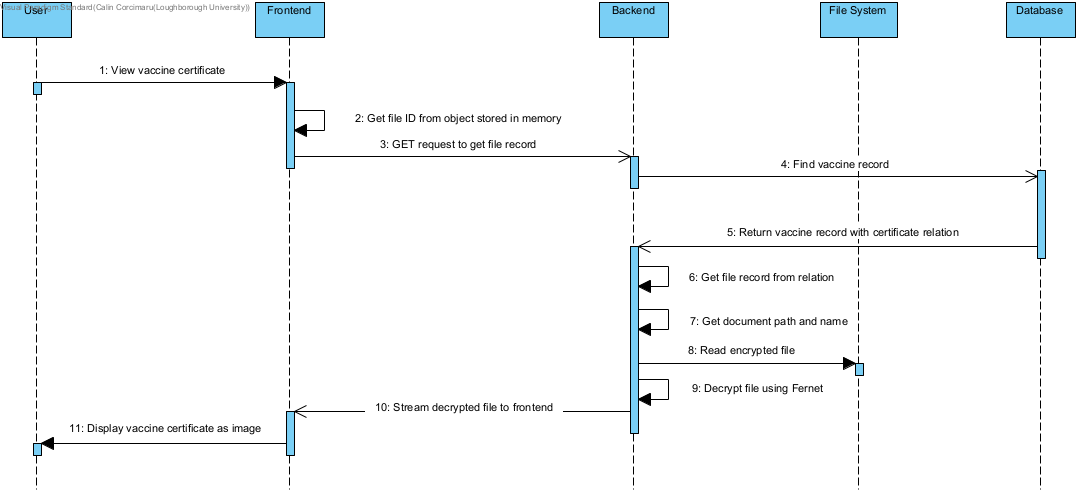
\includegraphics[width=\textwidth]{Sequence_FileView.png}\label{fig:seqfileview}} 
  \caption{Sequence Diagrams for File Upload and File View}\label{fig:fileuploadview}
\end{figure}

\FloatBarrier{}

The endpoint can be seen below:

\begin{lstlisting}[language=Python, caption=File Download Endpoint]
# Get a file by ID
@app.get("/files/{record_type}/{record_id}")
async def get_file(
  record_type: str,
  record_id: uuid.UUID,
  user_id: User = Depends(validate_session),
  session: Session = Depends(get_session)    
):    
  # Code to get the file record from the database
  
  async def get_data_from_file():
    with open(file_record.file_path, "rb") as f:
      encrypted_content = f.read()
      
    decrypted_content = decrypt_file(encrypted_content)

    yield decrypted_content
    
  return StreamingResponse(
    content=get_data_from_file(),
    media_type=file_record.file_type,
    status_code=status.HTTP_200_OK,
    headers={"Content-Disposition": f"inline; filename={file_record.name}"}
  )
\end{lstlisting}

Finally, the frontend was made with both mobile and desktop browsers in mind. This was achieved by using PrimeVue components and styling them with TailwindCSS. The system was also made to be responsive, so that it would look good on any screen size. Examples of the allergies page on both desktop and mobile can be seen below:

\begin{figure}[ht]
  \centering
  \subfloat[Desktop version]{%
      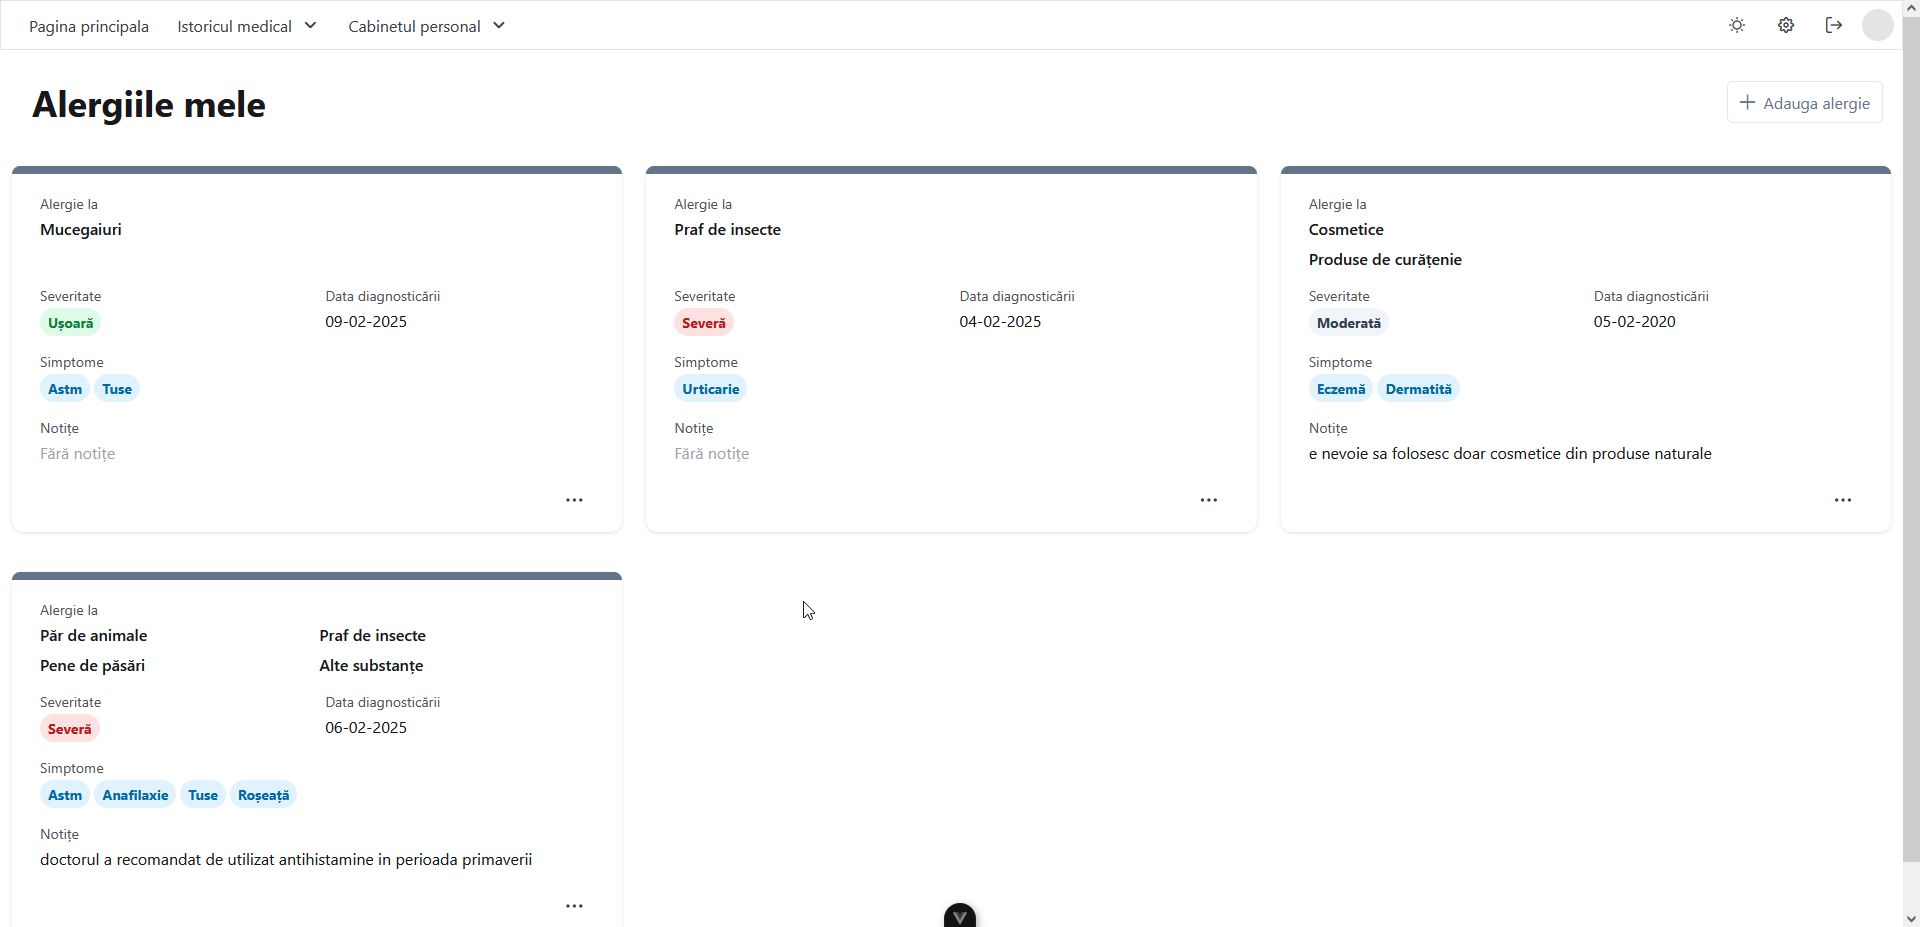
\includegraphics[width=\textwidth]{Desktop_AllergyView.png}%
  }
  \\[\baselineskip]
  \subfloat[Mobile version]{%
      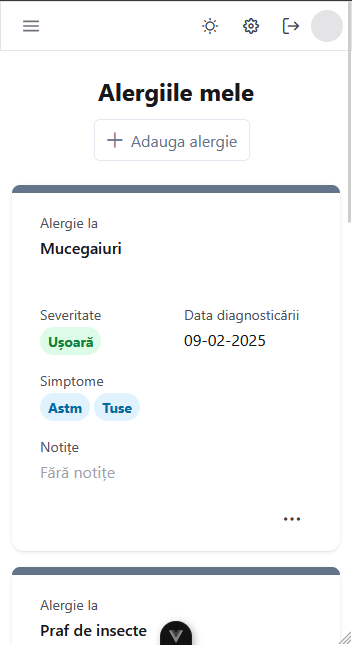
\includegraphics[width=0.4\textwidth]{Mobile_AllergyView.png}%
  }
  \caption{Desktop and Mobile version of the Allergies page}\label{fig:allergiespage}
\end{figure}

\FloatBarrier{}

\subsection{Challenges}

\subsubsection{Introducing new functionality}

In this sprint, the main challenge was introducing the new features/functionality in the system, while ensuring they worked properly together with both the existing frontend and backend. For some features, there was a need to revise and change some of the existing code, such as the API endpoints and even the database schemas to accommodate the newly implemented changes. This added some additional complexity, as it was crucial to ensure the changes did not break any of the existing functionality, while allowing the new features to work as intended.

\subsubsection{File Uploads}

Another challenge was understanding how some of the newly implemented features worked, such as the file upload system. It is important to note that the student had no previous experience implementing any file upload functionality, so extra time and work was dedicated to ensure the relevant documentation was studied and then implemented correctly.

\subsubsection{System complexity}

Finally, due to lack of time and poor initial planning because of the complexity of the system, some of the features intended for this sprint had to be moved to the next one. Some examples include the health data section and also the main dashboard parts for vaccines, allergies, medications and health data. 

These changes and challenges show that undertaking a more agile approach to the project was beneficial, as the project embraces change and allows for more flexibility in the development process.

\subsection{Requirements completed}

The main requirements completed in this sprint were:

\begin{itemize}
    \item The system must store the data in a secure manner, ensuring that only the patient and the doctor can access the data.
    \item The system must allow patients to upload their own medical records in a variety of formats (PDF, DOC, etc).
    \item The system should allow to upload files/documents for other types of records (vaccine certificates, etc).
    \item The system must allow the patient to add their own allergies.
    \item The system must allow the patient to add their own vaccinations.
    \item The system must allow patients to enter their current medication including details such as the name of the drug, dosage, frequency and start/end date.
    \item The system must allow patients to add new medication to their list.
\end{itemize}

\section{Sprint \#3}

The third sprint of the project was focused on building the main dashboard view of the system, which would display an overview of the most recent records added, such as vaccines, allergies, medications, etc. Additionally, another aim for this sprint was to complete the vital signs feature of the system, which would allow patients to add information such as weight or blood pressure in both a tabular and graphical format. 

All these features were part of the initial requirements discussed with the stakeholders, and were chosen to be completed in this sprint as their technical implementation was similar to more complex features that would be implemented in the future, which would help build additional proficiency in the frameworks and libraries used in the project.

However, besides the above-mentioned features, additional work had to be done on how the information is displayed in the frontend. This was a change requested by one of the stakeholders, based on their feedback after the sprint 2 features were presented to them. As such, additional time had to be spent on reworking the frontend to better display the information in a more user-friendly and consistent way. 

\subsection{Updated frontend}

One of the main feedback received from the stakeholders was the inconsistency in how the information was displayed for some of the sections in the system, such as the vaccines, allergies and medications. This was due to the different amount of information each record contained: vaccines contained the least amount of information, followed by allergies and medications. As such, some records were stored in a grid view, while others were stored in a list view. Also, some cards had different ways of displaying the information, such as using tags or colored lines, etc. 

The decision was made to keep things simple, by removing unnecessary colors and ensuring that there would be consistency in how the cards were displayed \- either by having only one type of view (grid/list) or offering both for the user to choose from. Tags were kept as they allowed for an easy way to display the information in a more readable way.

Thankfully, PrimeVue offered an easy way to re-work the frontend thanks to its Data View component \- a flexible component that could be used to display data in a grid or list view. The component also offered a way to customize the data displayed, such as adding tags, icons, etc. 

An example of the updated allergies page can be seen below in figure~\ref{fig:allergiespagev2}. The page now offers both a grid and list view, which can be toggled by the user. The page also offers a more consistent way of displaying the information, with each card containing the same information, but displayed in a different way depending on the view chosen.

\begin{figure}[ht]
  \centering
  \subfloat[Desktop version]{%
      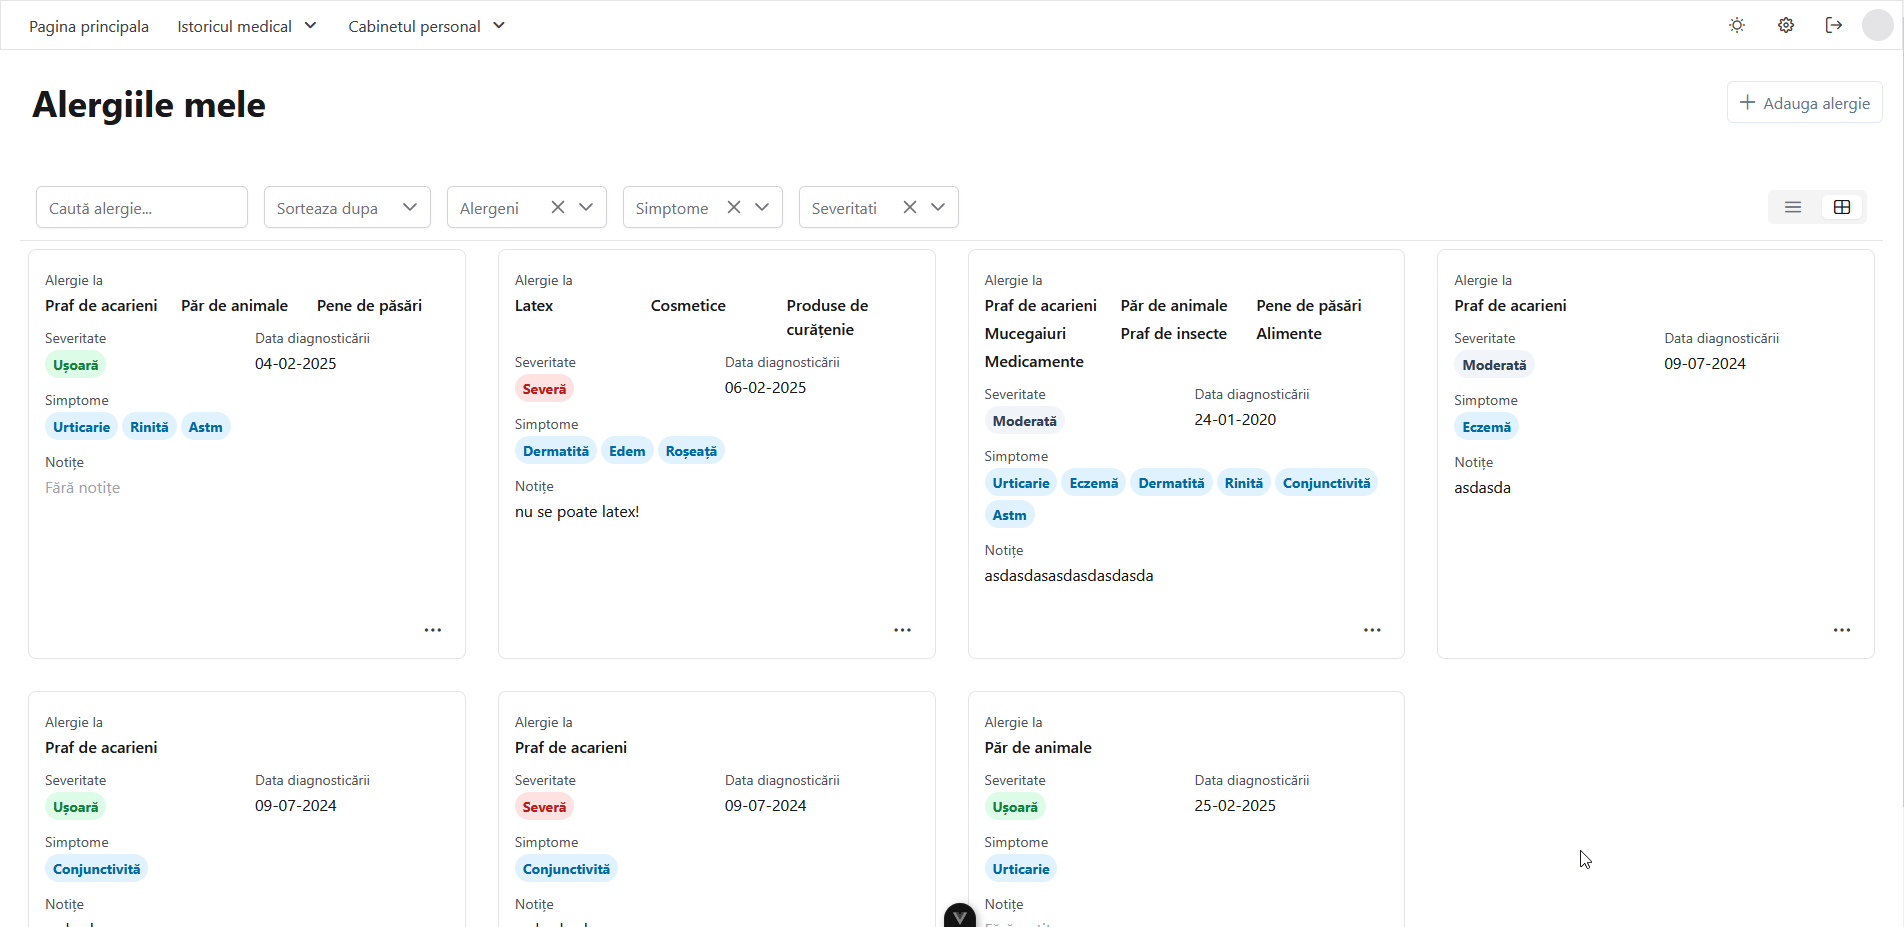
\includegraphics[width=\textwidth]{Desktop_AllergyView_v2.png}%
  }
  \\[\baselineskip]
  \subfloat[Mobile version]{%
      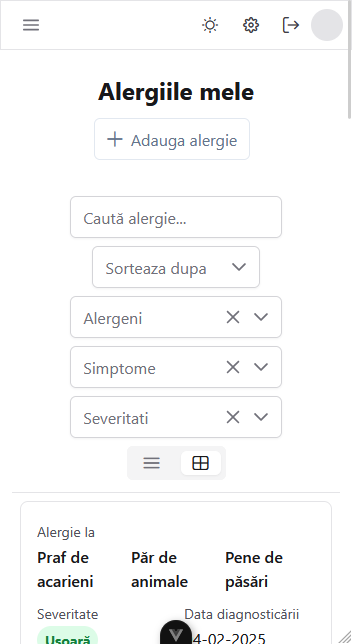
\includegraphics[width=0.4\textwidth]{Mobile_AllergyView_v2.png}%
  }
  \caption{Desktop and Mobile version of the Allergies page \- 2nd version}\label{fig:allergiespagev2}
\end{figure}

\FloatBarrier{}

\subsection{Filtering and sorting}

Another feedback provided by the stakeholders was the ability to filter and sort the information displayed in the system. This was especially important for the medications, where a patient could have multiple medications and would want to quickly find a specific one. Suggestions for this feature was to mainly add a search bar that would allow the user to find a specific record, however the stakeholders added that it would be nice to have some sorting/filtering options like sorting by date added or filtering based on type of medication, allergy severity, etc.

Sorting and filtering was implemented in the frontend by using Vue's reactivity system, powered by the ref and computed functions. The ref function was used to create reactive variables that would be updated whenever the data changed. The computed function was used to create computed properties that would be updated whenever the reactive variables changed. As such the sort query could be stored within a reactive variable, while the computed function would change the data displayed based on the sort query.

An example of the sorting and filtering functionality can be seen below:

\begin{lstlisting}[language=HTML, caption=Medication Sorting and Filtering]
  const filteredMedicine = computed(() => {
    return props.medications.filter((medication) => {
      return medication.name.toLowerCase().includes(searchQuery.value.toLowerCase())
    })
  })
\end{lstlisting}

\begin{lstlisting}[language=HTML, caption=Allergies Sorting and Filtering]
  const filteredAllergies = computed(() => {
  
  if (selectedAllergens.value.length > 0) {
    return props.allergies.filter((allergy) =>
      allergy.allergens.some((allergen) => selectedAllergens.value.includes(allergen))
    )
  }

  if (selectedReactions.value.length > 0) {
    return props.allergies.filter((allergy) =>
      allergy.reactions.some((reaction) => selectedReactions.value.includes(reaction))
    )
  }

  if (selectedSeverities.value.length > 0) {
    return props.allergies.filter((allergy) =>
      selectedSeverities.value.includes(allergy.severity)
    )
  }  

  return props.allergies.filter((allergy) =>
    allergy.allergens.some((allergen) =>
      allergen.toLowerCase().includes(searchQuery.value.toLowerCase())
    )
  )
})  
\end{lstlisting}

\subsection{Vital Signs}

Coming back to the sprint's focus, one of the main features intended to be implemented was the vital signs feature. This feature would allow the patient to add their own vital signs, such as weight, height, blood pressure, etc. The data would be displayed in both a tabular and graphical format, allowing the patient to see their progress over time.

When discussing this requirement with the stakeholders, a suggestion was given to display the most recent/current health data point added in a separate card, so that a patient could view their most recently added information easily. Additionally, a suggestion was given to display an arrow/icon near the value of the vital data point to show whether the value was above or below versus the previous value.

To display the data in a tabular and graphical view, the system uses PrimeVue's Data Table component and Chart.js library respectively. Examples of how the Vitals page looks can be seen below in figure~\ref{fig:vitalspage} and~\ref{fig:vitalspagegraph}.

\begin{figure}[ht]
  \centering
  \subfloat[Desktop version]{%
      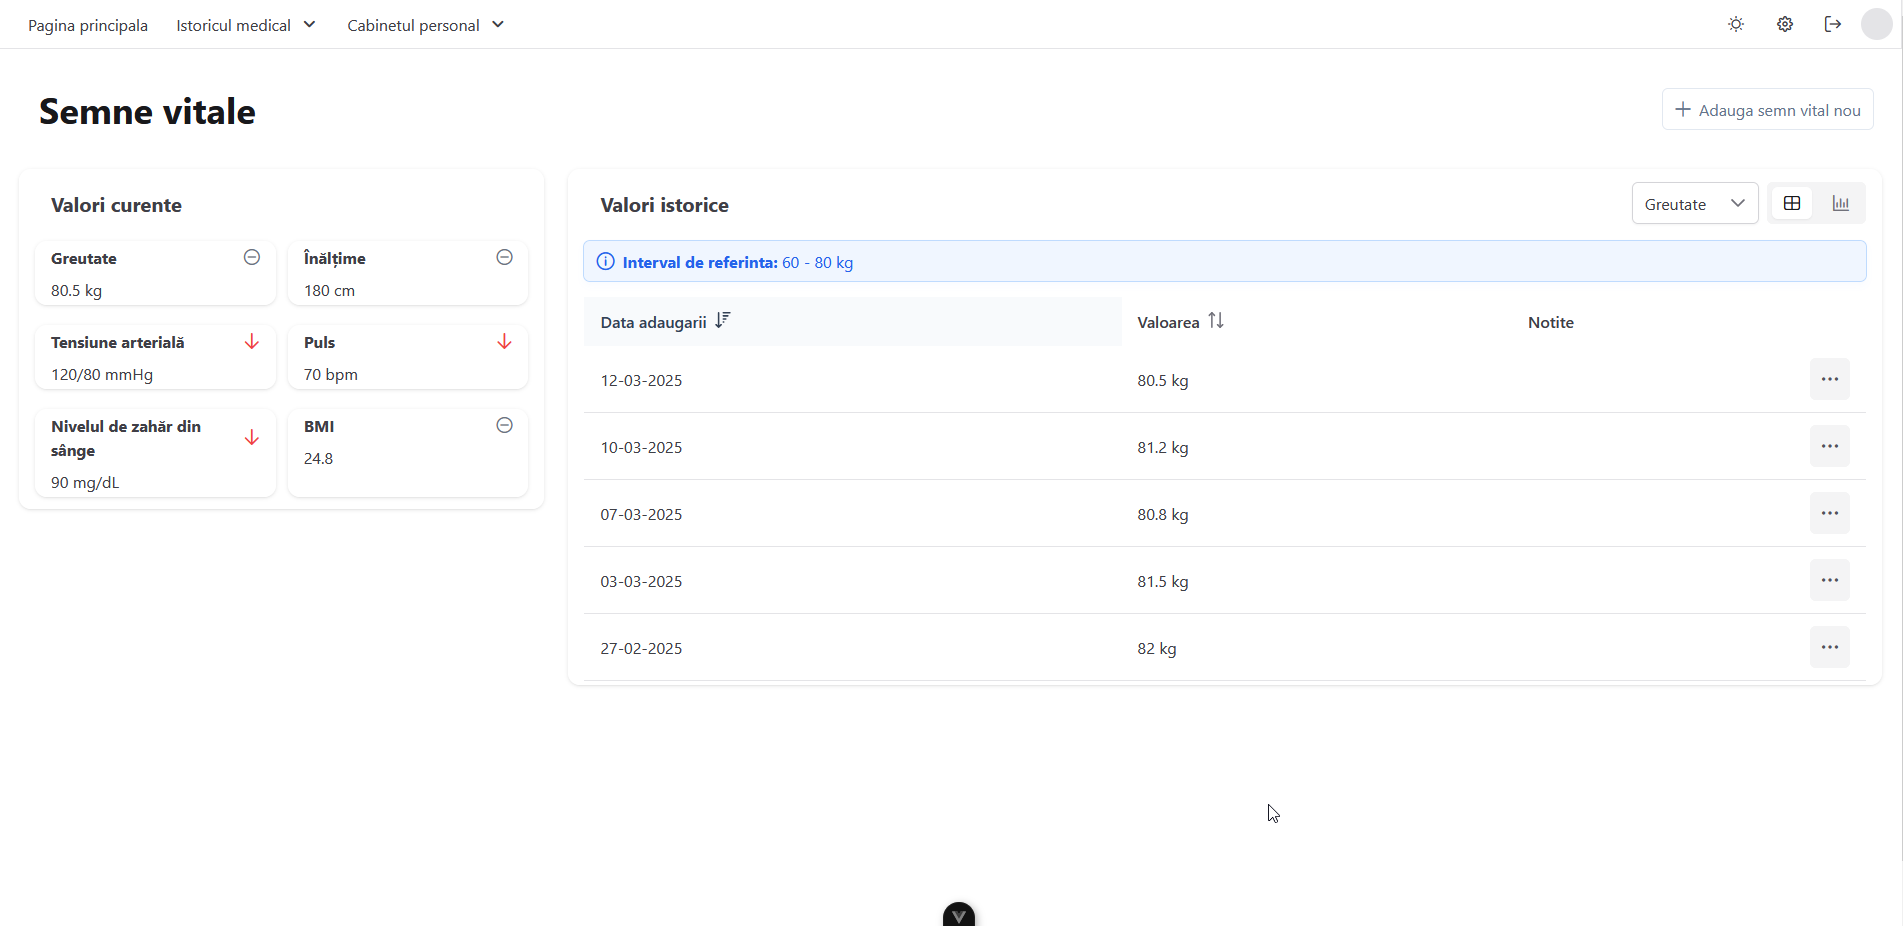
\includegraphics[width=\textwidth]{Desktop_VitalsView.png}%
  }
  \\[\baselineskip]
  \subfloat[Mobile version]{%
      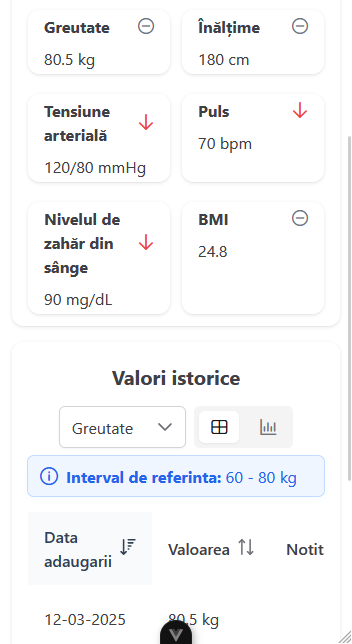
\includegraphics[width=0.4\textwidth]{Mobile_VitalsView.png}%
  }
  \caption{Desktop and Mobile version of the Vitals page}\label{fig:vitalspage}
\end{figure}

\FloatBarrier{}

\begin{figure}[ht]
  \centering
  \subfloat[Desktop version]{%
      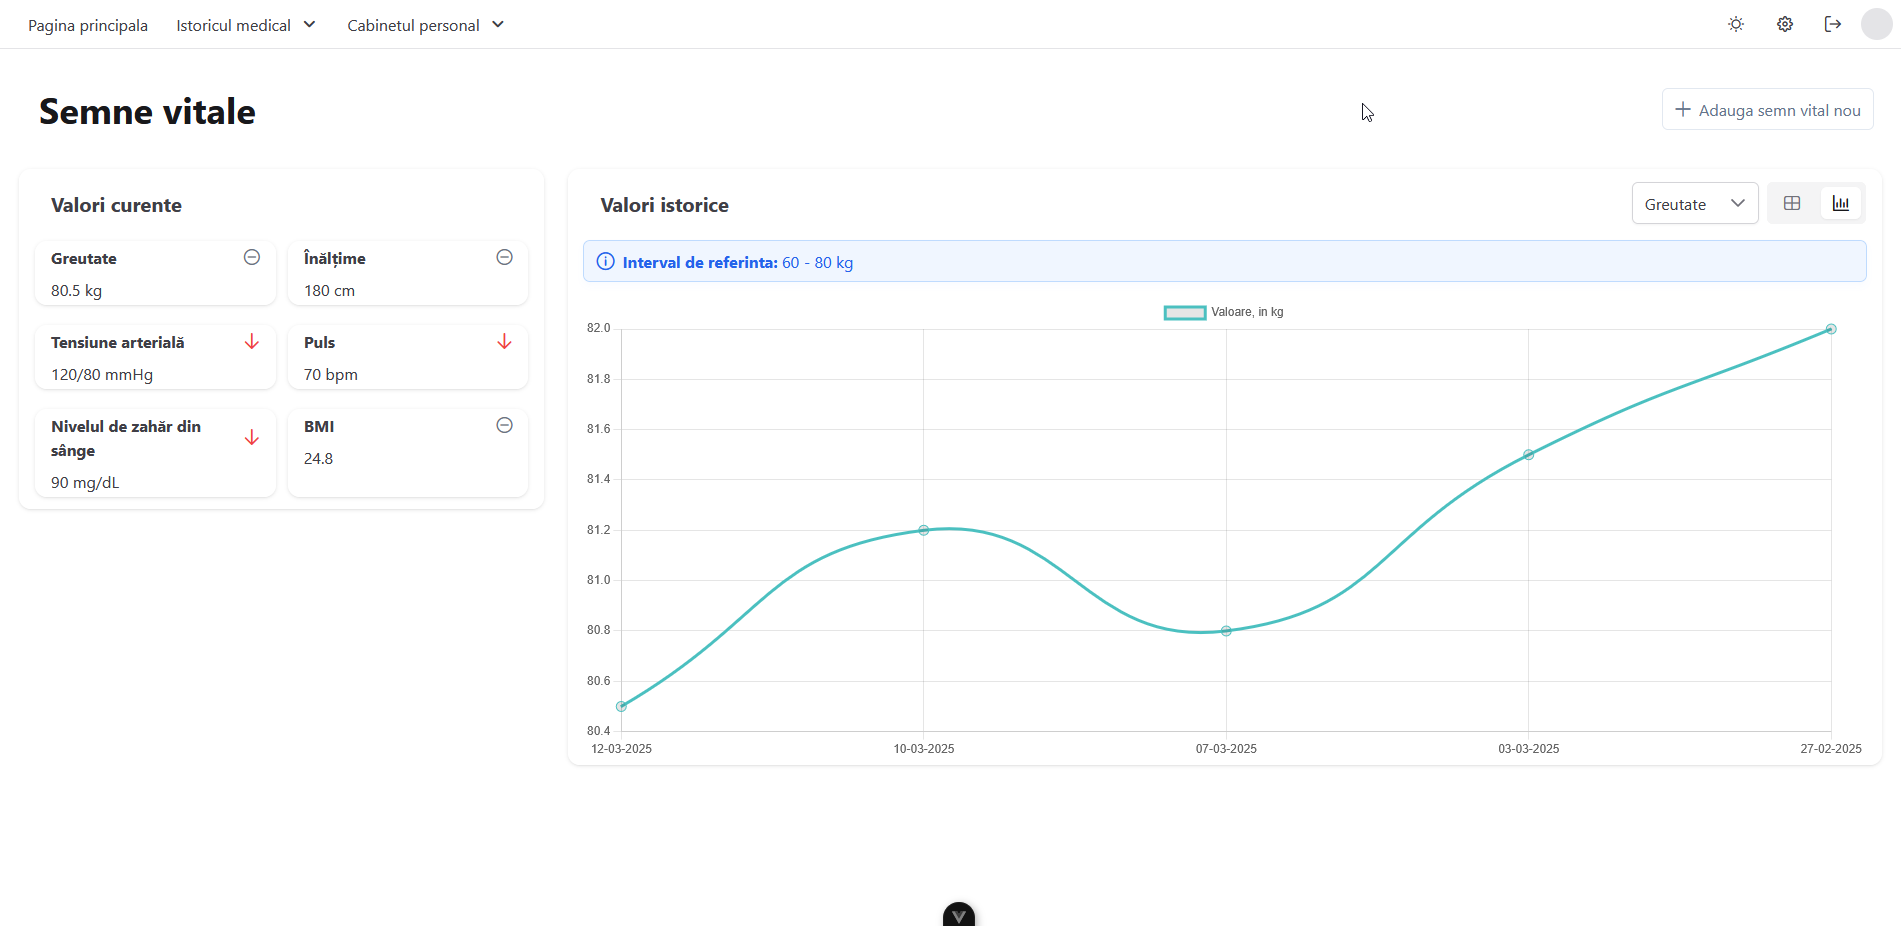
\includegraphics[width=\textwidth]{Desktop_VitalsView_Graph.png}%
  }
  \\[\baselineskip]
  \subfloat[Mobile version]{%
      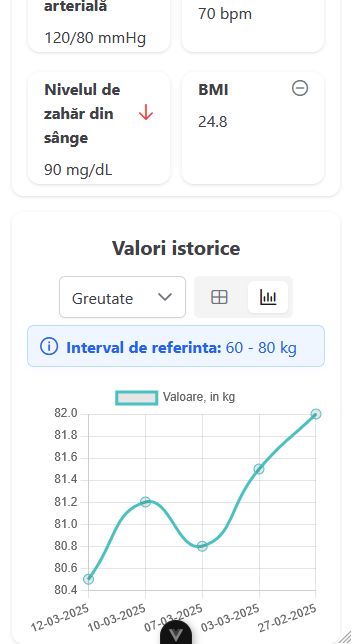
\includegraphics[width=0.4\textwidth]{Mobile_VitalsView_Graph.png}%
  }
  \caption{Desktop and Mobile version of the Vitals page, with Graph}\label{fig:vitalspagegraph}
\end{figure}

\FloatBarrier{}

\subsection{Dashboard}

Finally, the other main feature added was the ability for patients to have a dashboard-type view of the most recent records/information added to their account. The decision was made to display only the 5 most recent records for each section, encouraging the user to go to their respective page if they wanted to see more or see the records in more detail. The structure of each record was kept similar as to how they were displayed in their own pages to maintain consistency, so things like tags were still used to ensure a patient would know what they are looking for at the dashboard.

Similar to the vital signs feature, the Data Table view component from PrimeVue was used to create the individual tables for each of the section, making the development of the dashboard feature simple and easy. Each section was an individual Vue component, which was then imported into the dashboard main Vue view. An example of a section code can be seen below:

\begin{lstlisting}[language=HTML, caption=Vital Signs Dashboard Section Component]
<template>
  <Card :pt="cardStyles" class="h-full">
    <template #title>
      <h2 class="text-xl font-bold p-4">Semne vitale recent adaugate</h2>
    </template>
    <template #content>
      <DataTable :value="props.vitals" removableSort>
        <Column field="name" header="Numele" sortable> </Column>
        <Column field="value" header="Valoarea" sortable>
          <template #body="slotProps">
            <span v-if="slotProps.data.value">
              {{ slotProps.data.value }} {{ slotProps.data.unit }}
            </span>
            <span v-else>
              {{ slotProps.data.value_systolic }}/{{ slotProps.data.value_diastolic }}
              {{ slotProps.data.unit }}
            </span>
          </template>
        </Column>
        <Column field="date_recorded" header="Data adaugarii" sortable>
          <template #body="slotProps">
            <span> {{ slotProps.data.original_date_recorded }} </span>
          </template>
        </Column>
      </DataTable>
    </template>
    <template #footer>
      <RouterLink to="/vitale" class="p-button p-button-text">Vezi toate semnele vitale</RouterLink>
    </template>
  </Card>
</template>
\end{lstlisting}

Finally, the dashboard view can be seen below in figure~\ref{fig:dashboardpage}.

\begin{figure}[ht]
  \centering
  \subfloat[Desktop version]{%
      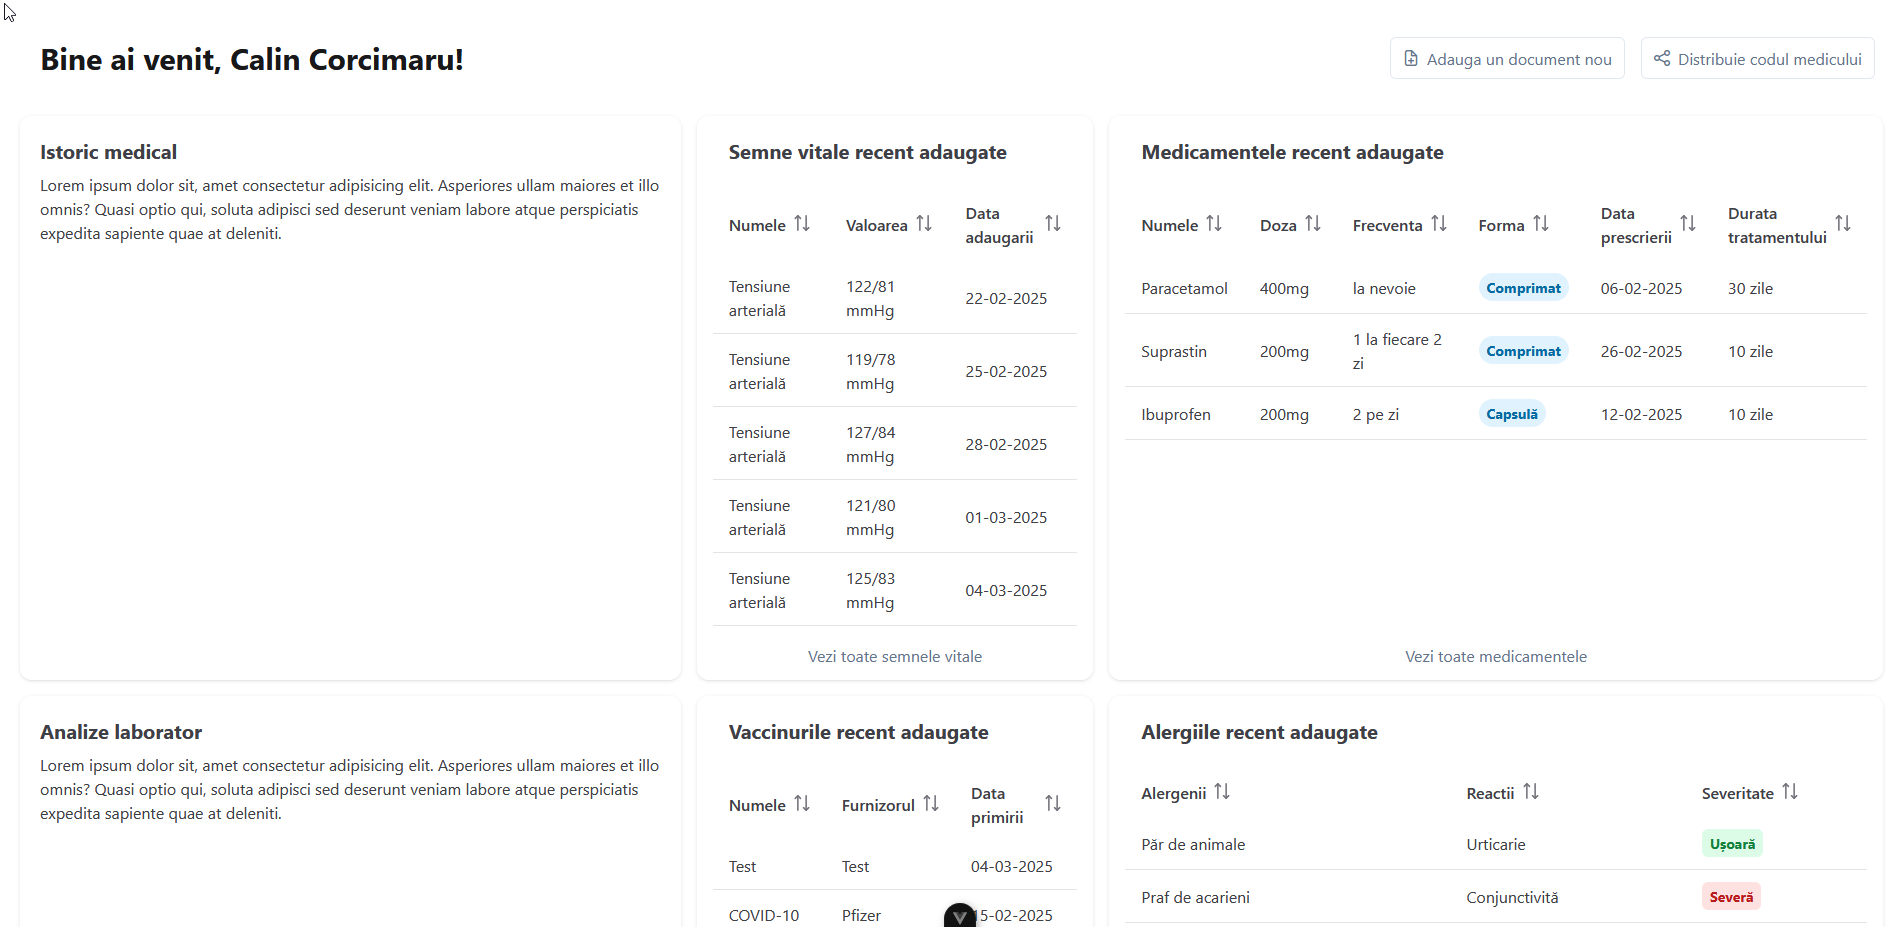
\includegraphics[width=\textwidth]{Desktop_DashboadView.png}%
  }
  \\[\baselineskip]
  \subfloat[Mobile version]{%
      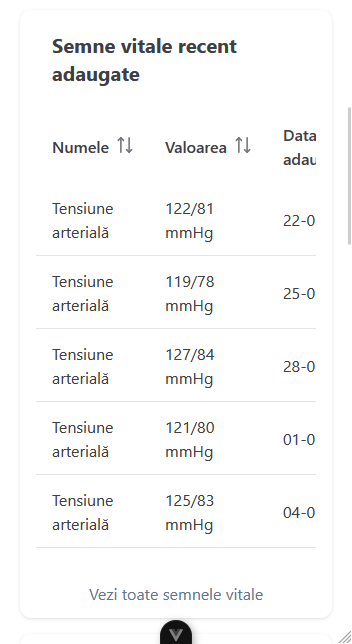
\includegraphics[width=0.4\textwidth]{Mobile_DashboardView.png}%
  }
  \caption{Desktop and Mobile version of the Dashboard page}\label{fig:dashboardpage}
\end{figure}

\FloatBarrier{}

\subsection{Backend changes}

While the focus of this sprint was mainly the frontend, there were some parts of the backend that needed to be changed to accommodate some of the implemented changes. 

One change made was the addition of a database table for the vital data points, which would contain the type name, such as Weight, the unit of measurement and a normal range, all of which was then used or displayed on the vitals page. Another change to the database was the addition of a new field, called date\_added to all of the tables/records in the system. This field was used mainly used to sort and determine the most recently added records to the system, which could be a different value to the other dates already used in the records' tables. An example could be found in vaccines: a vaccine could've been received years ago, but it could be added anytime to the system. As such, the record can have 2 different dates associated with it: the date the vaccine was actually received and the date it was added to the system. As such, the updated database schema can be found below:

\noindent\begin{minipage}{\textwidth}
  \begin{center}
      \rotatebox[origin=c]{270}{
          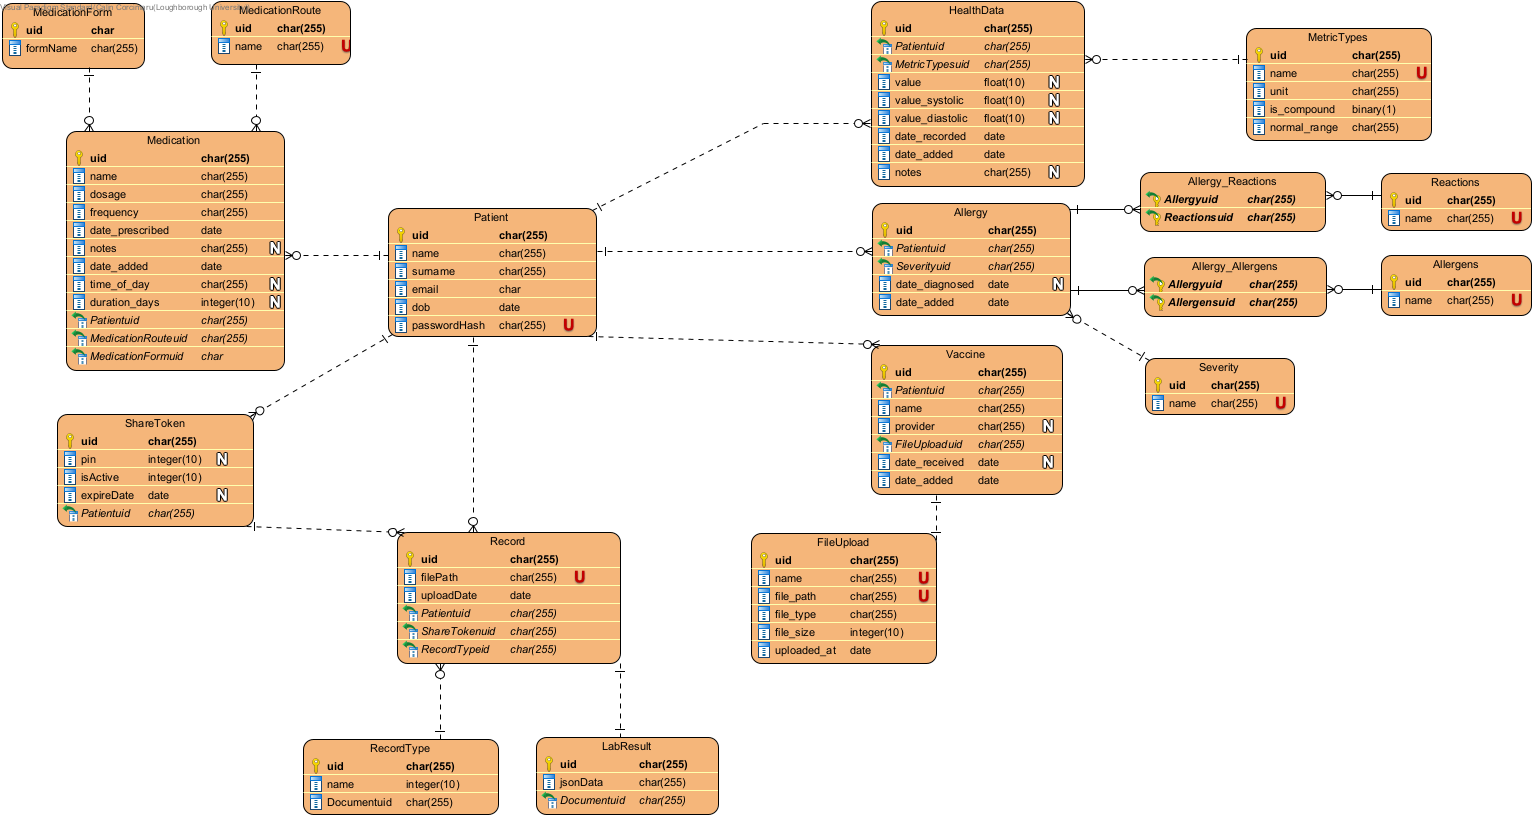
\includegraphics[width=0.95\textheight,keepaspectratio]{ERD_updatedS3.png}
      }
      \captionof{figure}{Updated Entity Relationship Diagram \- Sprint \#3}\label{fig:erd_s3}
  \end{center}
\end{minipage}

Other changes included multiple changes to the API endpoints, mainly relating to the vital signs data, due to the addition of the new table and its contents. Similarly, a new endpoint for the dashboard had to be created, which would use the newly added date\_added field to sort through the 5 most recent records in each category and send them back as the response. Below can be found the code that sorts and selects the 5 most recent records for each category:

\begin{lstlisting}[language=Python, caption=Dashboard Endpoint]
@app.get("/dashboard", response_model=UserDashboard)
async def get_dashboard(user_id: uuid.UUID = Depends(validate_session), session: Session = Depends(get_session)):
    user = session.get(User, user_id)
    
    if user_id != user.id:
        raise HTTPException(status_code=403, detail="You do not have permission to access this endpoint!")   
    
    newest_vaccines = session.exec(select(Vaccine).where(Vaccine.user_id == user_id).order_by(col(Vaccine.date_added).desc()).limit(5)).all()
    newest_allergies = session.exec(select(Allergy).where(Allergy.user_id == user_id).order_by(col(Allergy.date_added).desc()).limit(5)).all()
    newest_healthdata = session.exec(select(HealthData).where(HealthData.user_id == user_id).order_by(col(HealthData.date_added).desc()).limit(5)).all()
    newest_medications = session.exec(select(Medication).where(Medication.user_id == user_id).order_by(col(Medication.date_added).desc()).limit(5)).all()
    
    # Code that transforms each record into a response object...

    user_dashboard = UserDashboard(
        id = user.id,
        name = user.name,
        vaccines = vaccines_response,
        allergies = allergies_response,
        vitals = healthdata_response,
        medications = medications_response
    )
    
    return user_dashboard
\end{lstlisting}

\subsection{Challenges}

\subsubsection{Scope Creep}

One of the main challenges encountered in this sprint was the scope creep and the change in requirements. While an initial discussion was done with stakeholders and wireframes were created to have a shared understanding regarding how the system should look, further discussions brought up areas of improvement and change opportunities within the system. This led to additional work being done on both the frontend and backend to ensure the system was adhering to stakeholder expectations, and that it provides a pleasant user experience and enough functionality to be a viable solution for the market.

\subsubsection{Infrequent communication with stakeholders}

One of the main problems encountered in this sprint and the previous ones was the infrequent communication with stakeholders. This was caused by many factors, such as the busy schedules of both the student and the stakeholders, their other commitments such as studies or other work positions, but also the fact that all communication was done virtually, limiting the interaction to meetings or messages via communication apps. This infrequent communication led to situations where the student might have had to make decisions regarding the system design on their own, which could not have been liked by stakeholders, requiring changes or re-doing, adding additional work load on the student. 

As such, it was clear that for the upcoming sprints, a more constant communication between the student and stakeholders needed to be established to ensure that what was worked on was in line with the stakeholders' expectations.

\subsubsection{Lack of proper testing procedures}

Due to the complexity of the system and time pressure, barely any kind of automated testing was implemented. This lead to unexpected issues appearing in the course of development, which created additional work for the student, changing their focus from the sprint items to fixing the bugs, thus delaying the sprint completion. The student also doesn't have much experience creating tests for the frontend, which made the testing process even more difficult, leading to many of the testing to be done manually or skipped entirely. Due to the limited time remaining, it might be necessary to dedicate a part of the upcoming sprints to do some more thorough testing to ensure that the system as a whole does not have any critical bugs or issues that may affect its functionality.

\subsection{Requirements completed}

\begin{itemize}
    \item The system must have a dashboard view which displays an overview of the most recent information added to the system (latest lab tests, doctor consultations, vaccinations etc).
    \item The system should display the health records in both a list or grid view.
    \item The system should allow the patient to enter vitals information, such as height, weight, blood pressure, etc.
    \item When multiple vital entries are made, the system could display a historical graph of the patient's vitals.
    % TODO: Add more requirements
\end{itemize}

\section{Sprint \#4}

The fourth sprint of the project focused on adding the ability to add health records, such as lab tests, doctor consultations or imaging results. This was one of the main features requested by the stakeholders, as it would allow a patient to have all their medical history in one place, making it easier for them to view and share it with their doctors.

Additionally, at the end of sprint \#3, the stakeholders provided feedback regarding the features implemented in the previous sprint. Some of the feedback included:

\begin{itemize}
    \item The graph in the Vitals page should show the normal range for that specific vital type in graph.
    \item The Vitals signs page should have a date filtering functionality to choose a date range for the signs displayed in the graph or table.
    \item Weight and height should not have a normal range.
    \item Previously, the trend most recent vitals signs were compared with the 2nd most recent ones, which was not a good choice for comparison. The most recent vitals signs should be compared with the normal range for that specific vital type.
    \item On the main dashboard, the most recent vitals section should show the most recent values for one each type of vital signs, instead of the most recent 5 values for each type.
    \item On the main dashboard, only the allergies with moderate and severe allergies should be displayed.
\end{itemize}

\subsection{Health Records}

As mentioned in the introduction to this section, the main focus of this sprint was creating the functionality to add health records such as lab tests, doctor consultations or imaging results in the system. This was a crucial feature and a main requirement of the system, as it would allow patients to create their medical history in the system, upload the files associated with these records and then refer to them whenever needed or share them with doctors to allow them to have a more accurate patient history and thus offer better treatment.

The choice was made to display the record history in a tabular format, as that would allow to display the important information in a readable way, but also to sort the information based on different fields such as the date of the consultation or filter by fields such as doctor or institution name for easier search. PrimeVue has a DataTable component, which allowed the inclusion of all these features with little effort that are displayed in a user-friendly way. An example of the health records page can be seen below in figure~\ref{fig:healthrecordspage}.

\begin{figure}[ht]
  \centering
  \subfloat[Desktop version]{%
      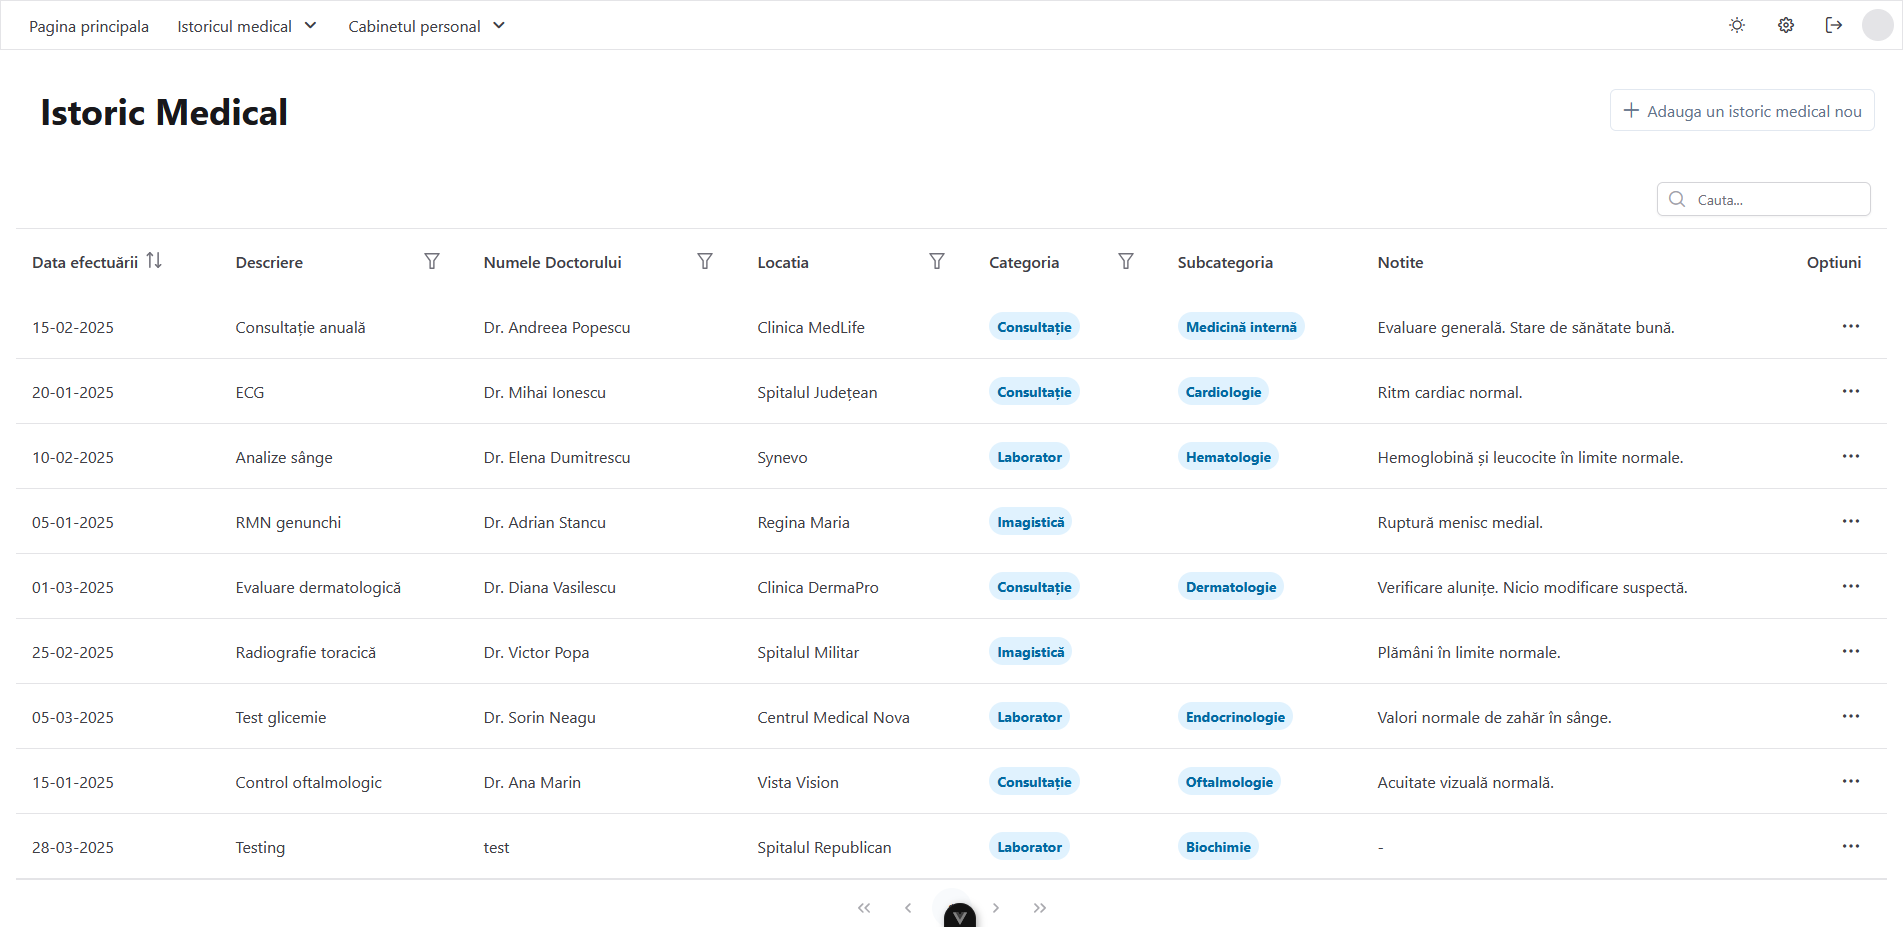
\includegraphics[width=\textwidth]{Desktop_HistoryView.png}%
  }
  \\[\baselineskip]
  \subfloat[Mobile version]{%
      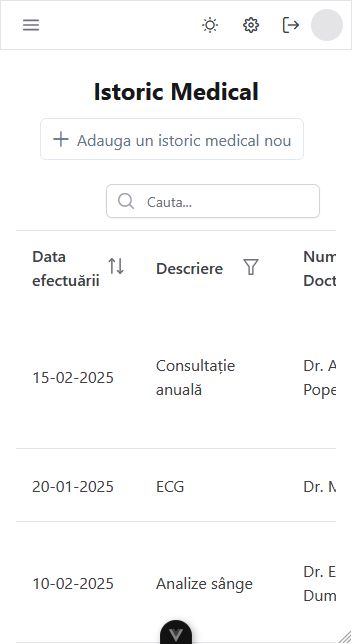
\includegraphics[width=0.4\textwidth]{Mobile_HistoryView.png}%
  }
  \caption{Desktop and Mobile version of the History page}\label{fig:healthrecordspage}
\end{figure}

\FloatBarrier{}

DataTable also comes with an in-built filtering option, which allowed to add a search bar for the whole table, but also search functions for specific fields. Example of the search bar can be seen in the screenshots above, and the filter menu can be seen below in figure~\ref{fig:filtermenu}. A code snippet of the filter function in a column can also be seen below.

\begin{figure}[htbp]
  \centering
  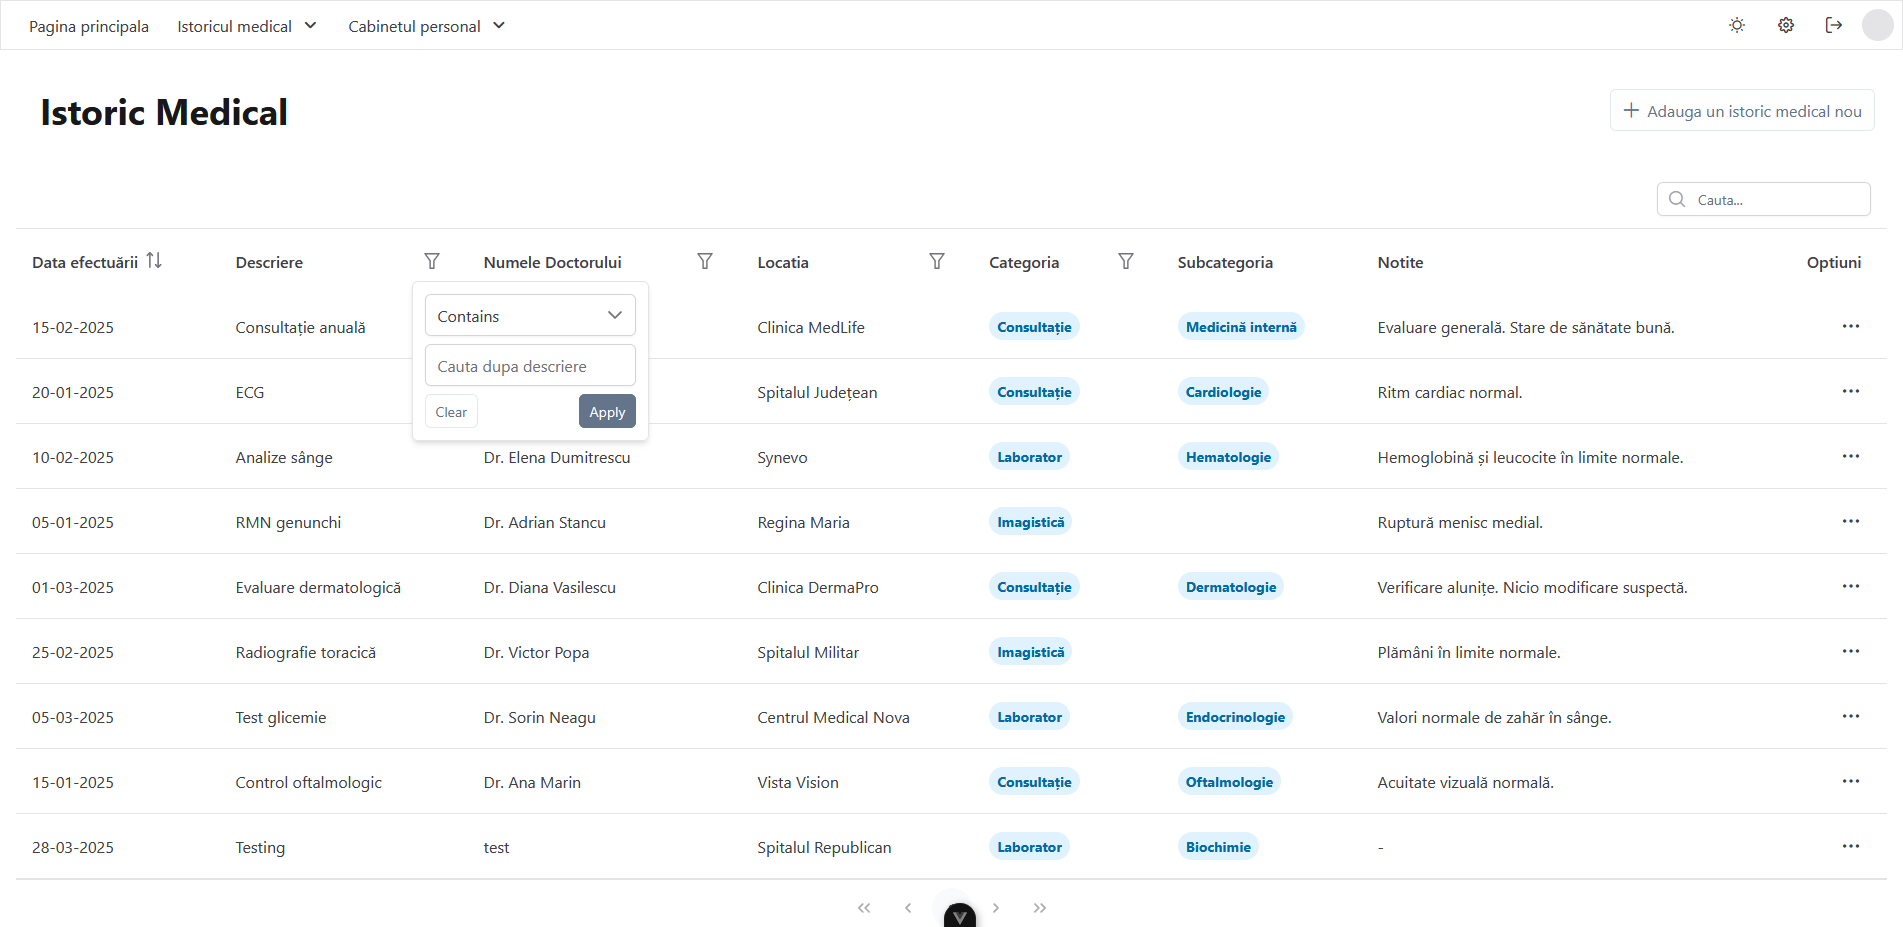
\includegraphics[width=\textwidth]{Desktop_HistoryView_Filter.png}
  \caption{Filter Menu for Health Records}\label{fig:filtermenu}
\end{figure}

\begin{lstlisting}[language=HTML, caption=Filter Function for Health Records]
  <template>
  <div class="h-full w-full px-4">
    <DataTable 
      v-model:filters="filters" 
      :value="history" 
      :rows="10" 
      paginator 
      dataKey="id" 
      filterDisplay="menu"
      :loading="loading"
      :globalFilterFields="['name', 'doctor_name', 'place', 'category']"
      removableSort
      responsiveLayout="stack"
      breakpoint="960px"
    >
      <template #header>
        <div class="flex justify-end">
          <IconField>
            <InputIcon>
              <i class="pi pi-search" />
            </InputIcon>
            <InputText size="small" v-model="filters['global'].value" placeholder="Cauta..." />
          </IconField>
        </div>
      </template>

      <!-- Previous columns here -->

      <Column field="doctor_name" header="Numele Doctorului" :showFilterMenu="true">
      <template #filter="{ filterModel, filterCallback }">
        <InputText v-model="filterModel.value" type="text" class="w-full" @input="filterCallback()" placeholder="Cauta dupa doctor" />
      </template>
    </Column>

    <!-- Next columns here -->
    </DataTable>
  </div>
</template>
\end{lstlisting}

Finally, with the addition of health records page, the ability to view and upload PDF files was also added to the system. This was an important feature to add, as files related to health records are usually sent in a PDF format. There was a slight challenge as to how to display the PDF files in the frontend, however in the end it was decided to use a simple approach that utilised in-built functionality through the use of object element from HTML. To allow mobile users to view the files, the system instead used a button to allow mobile users to download the file, as mobile browsers do not support the object element. The code for the PDF viewer can be seen below and a screenshot in figure~\ref{fig:pdfviewer}.

\begin{lstlisting}[language=HTML, caption=PDF viewer Function for Health]<template>
  <Dialog
    v-model:visible="visible"
    modal
    header="Vizualizeaza fisierul"
    class="w-full md:w-3/4 md:h-3/4"
    @hide="emit('close')"
  >
    <div v-if="metadata?.file_type == 'application/pdf'">
      <object
        :data="`http://localhost:8000/files/medicalhistory/${props.historyId}`"
        type="application/pdf"
        class="w-full h-[70vh] hidden md:block"
      />
      <div class="block md:hidden text-center mt-2">
        <a
          :href="`http://localhost:8000/files/medicalhistory/${props.historyId}`"
          target="_blank"
          class="bg-blue-500 text-white px-4 py-2 rounded-md inline-block mb-4"
        >
          Deschide certificatul PDF
        </a>
      </div>
    </div>
    <Image
      v-else
      :src="`http://localhost:8000/files/medicalhistory/${props.historyId}`"
      alt="Fisier consultatie"
      class="w-full h-screen"
      preview
    />
  </Dialog>
</template>
\end{lstlisting}

\begin{figure}[ht]
  \centering
  \subfloat[Desktop version]{%
      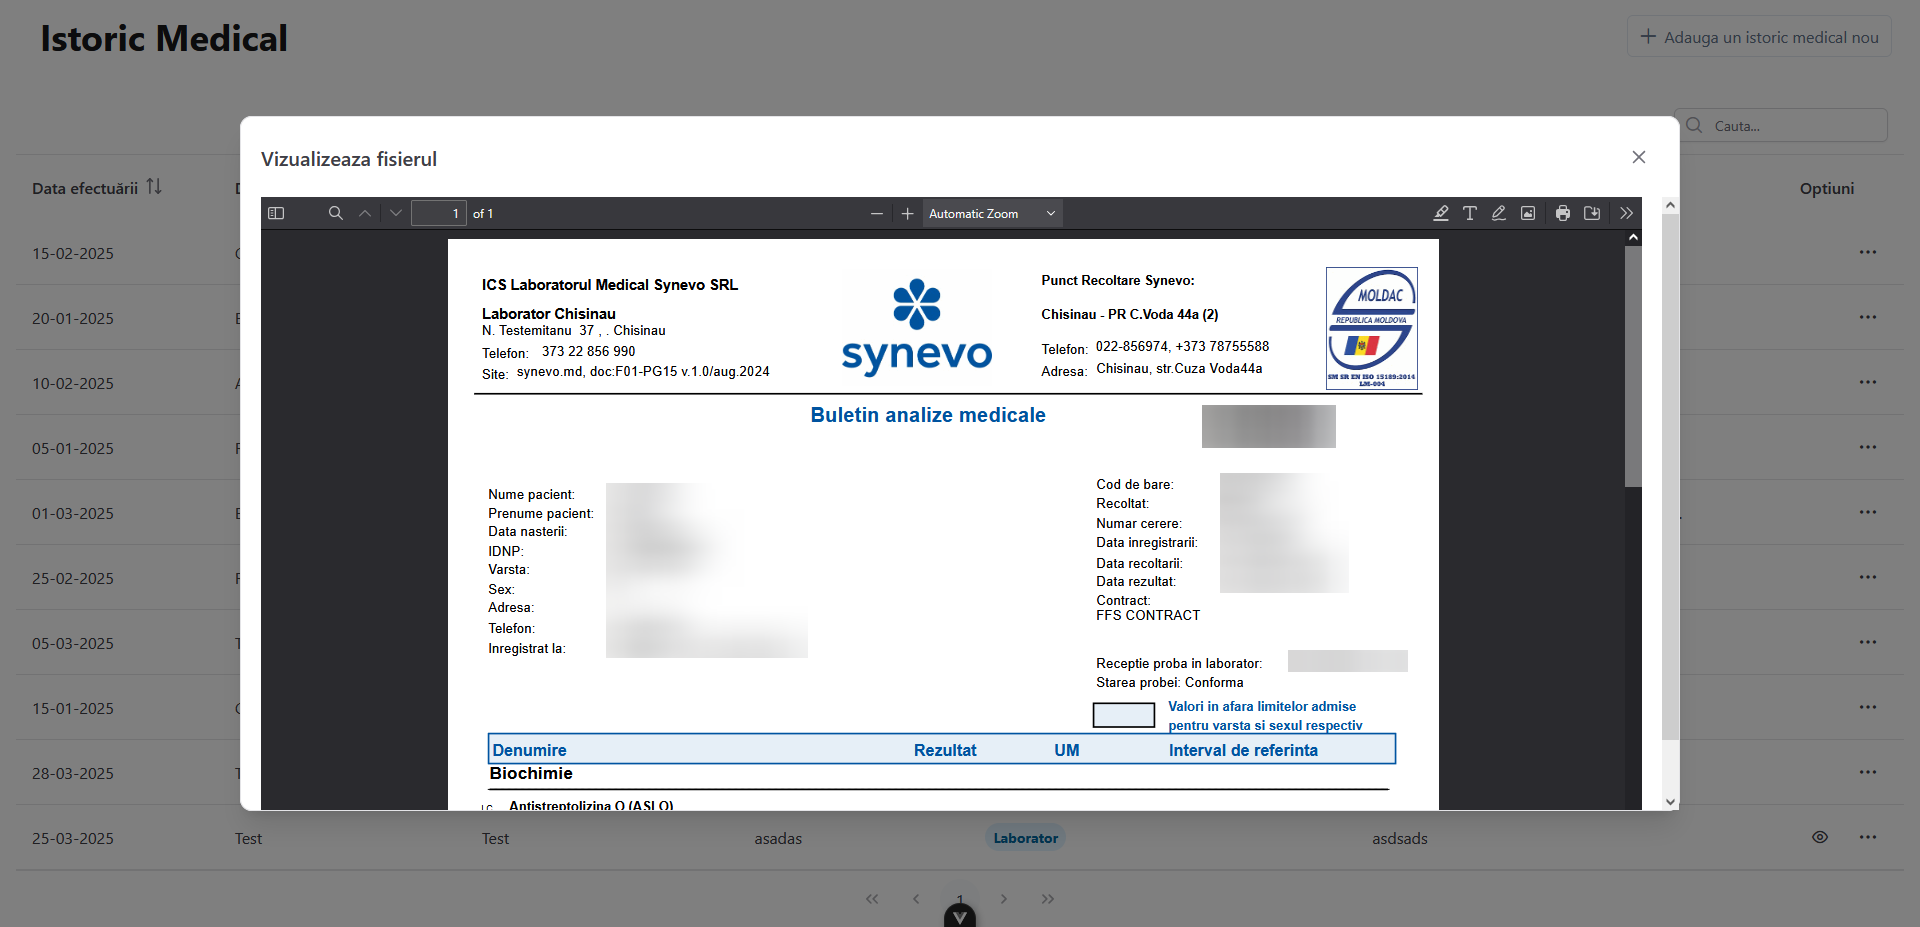
\includegraphics[width=\textwidth]{Desktop_History_PDF.png}%
  }
  \\[\baselineskip]
  \subfloat[Mobile version]{%
      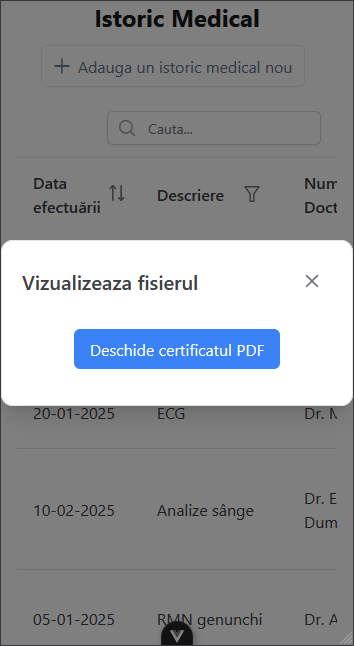
\includegraphics[width=0.4\textwidth]{Mobile_History_PDF.png}%
  }
  \caption{Desktop and Mobile version of the PDF viewer}\label{fig:pdfviewer}
\end{figure}

\FloatBarrier{}

\subsection{Backend changes}

To enable the health record functionality to work properly, new tables had to be created in the database to store the records: MedicalHistory for the main table, MedicalCategory for main categories of the records (lab tests, doctor consultations, etc) and additional tables like MedicalSubCategory and LabSubcategory for the subcategories of the records (blood test, urine test, etc). The new tables can be seen below in figure~\ref{fig:erd_s4}.

\noindent\begin{minipage}{\textwidth}
  \begin{center}
      \rotatebox[origin=c]{270}{
          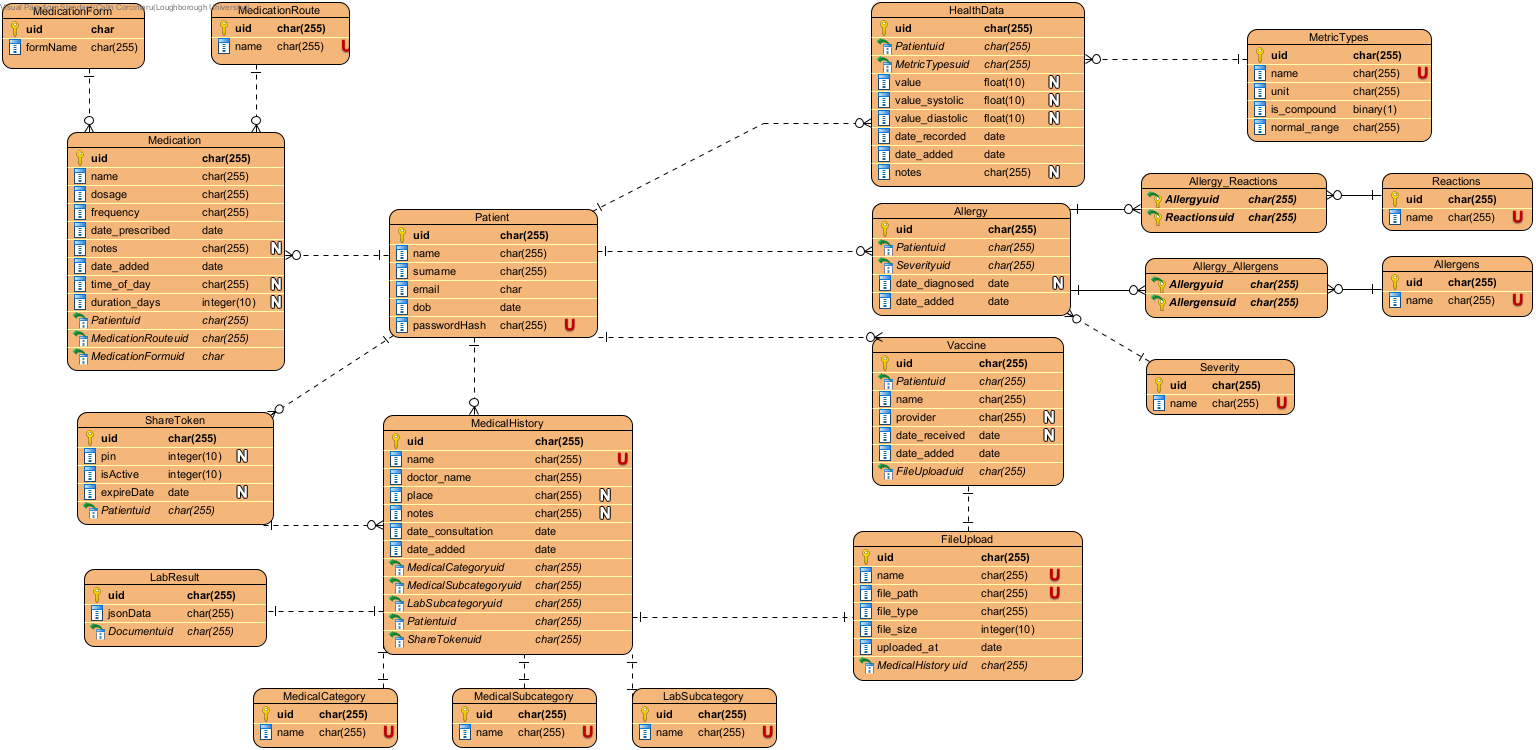
\includegraphics[width=0.95\textheight,keepaspectratio]{ERD_updatedS4.png}
      }
      \captionof{figure}{Updated Entity Relationship Diagram \- Sprint \#4}\label{fig:erd_s4}
  \end{center}
\end{minipage}

\FloatBarrier{}

Additionally, endpoints were created to allow the user to add, edit and delete health records. The endpoints were created in a similar way to the other endpoints in the system, using FastAPI and SQLModel.

\subsection{Work on stakeholder feedback}

As mentioned in the section introduction, in this sprint work was done to address the feedback received from stakeholder meetings regarding the features implemented in the previous sprint.

The biggest changes were related to how the vital signs are displayed and filtered in the system. The graph now shows lines for the upper and lower ranges for the respective vital signs, and a date range filter was added to the page, allowing the user to select a date range for the data displayed in the graph. 

Additionally, the most recent vitals are now compared to the normal range instead of the previous value. This change was implemented to ensure the normal range is used effectively to show whether their vitals signs are within or outside of it to allow for more informed decision making. These changes can be seen below in figure~\ref{fig:vitalchanges}.

\begin{figure}[htbp]
  \centering
  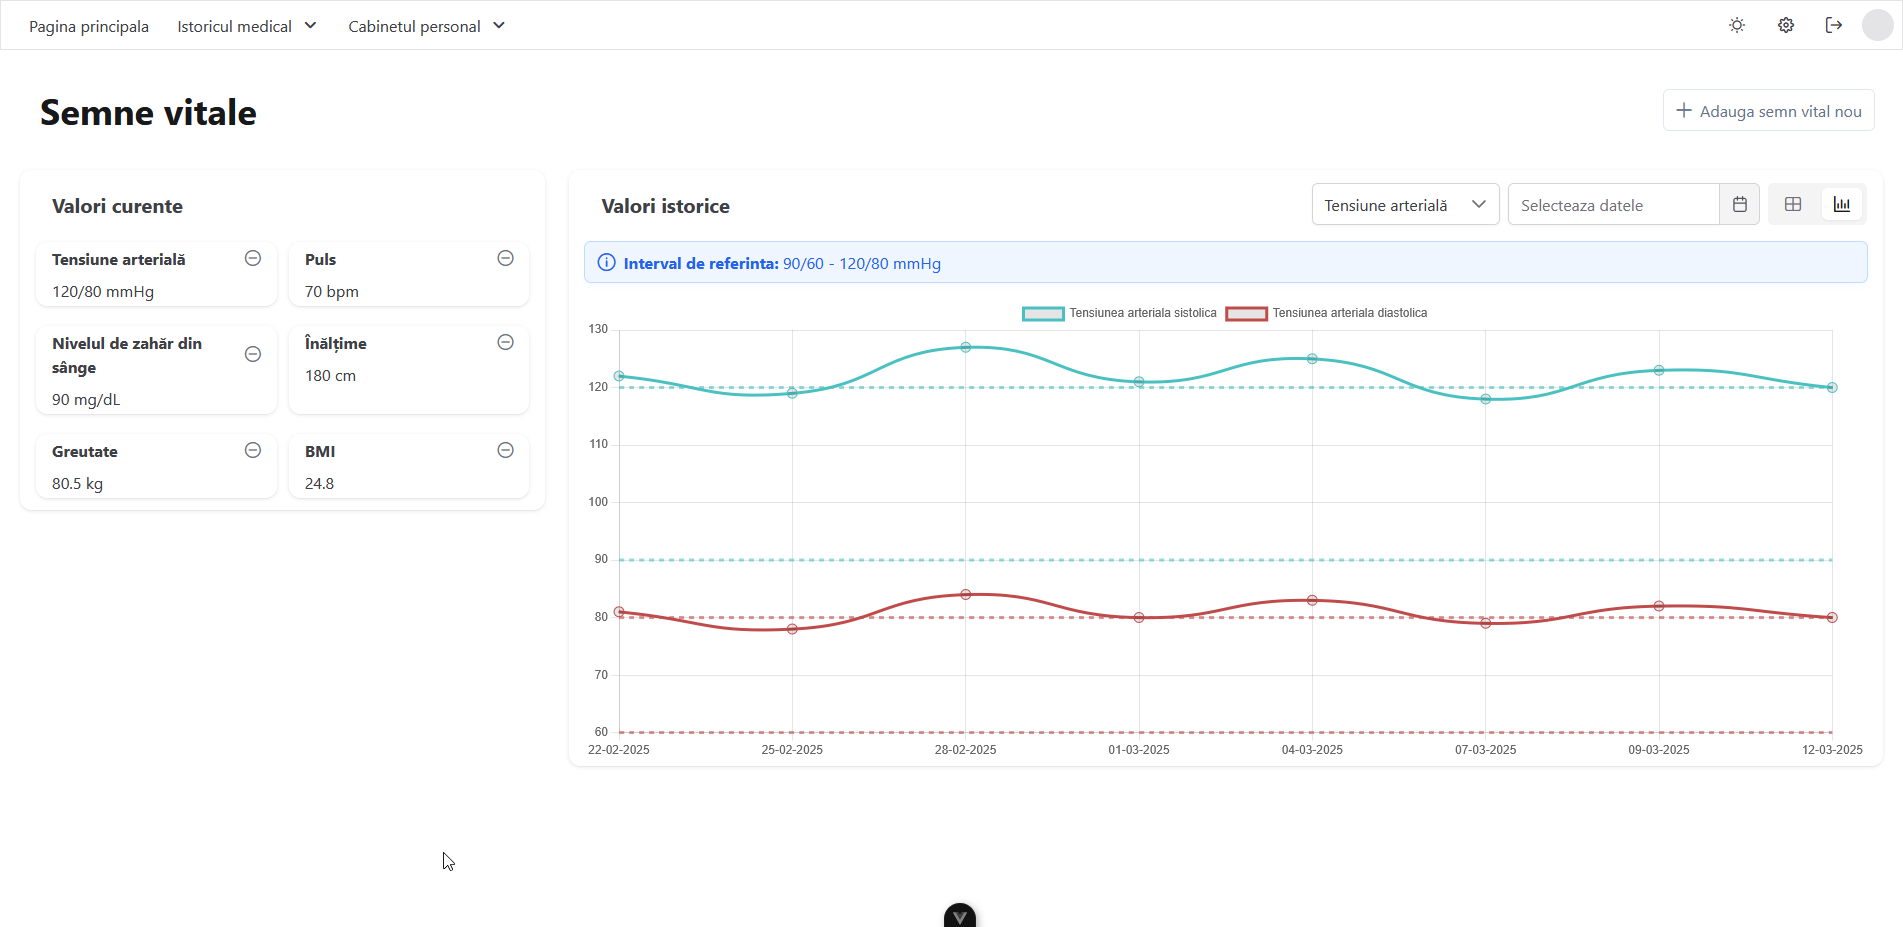
\includegraphics[width=\textwidth]{Desktop_Vitals_Updated.png}
  \caption{Updated Vitals View based on stakeholder feedback}\label{fig:vitalchanges}
\end{figure}

\FloatBarrier{}

The main dashboard page was also slightly changed to show the most recent vitals signs for each type of vital sign, instead of the most recent 5 values for each type. This was done to ensure that the dashboard page is not cluttered with too much information and that the user can easily see their most recent vitals signs.

Finally, the allergies section on the dashboard page was also changed to only show the moderate and severe allergies, as it was suggested by the stakeholders that this would be more useful for patients to track their most important allergies. The new dashboard can be seen below in figure~\ref{fig:dashboardchanges}.

\begin{figure}[htbp]
  \centering
  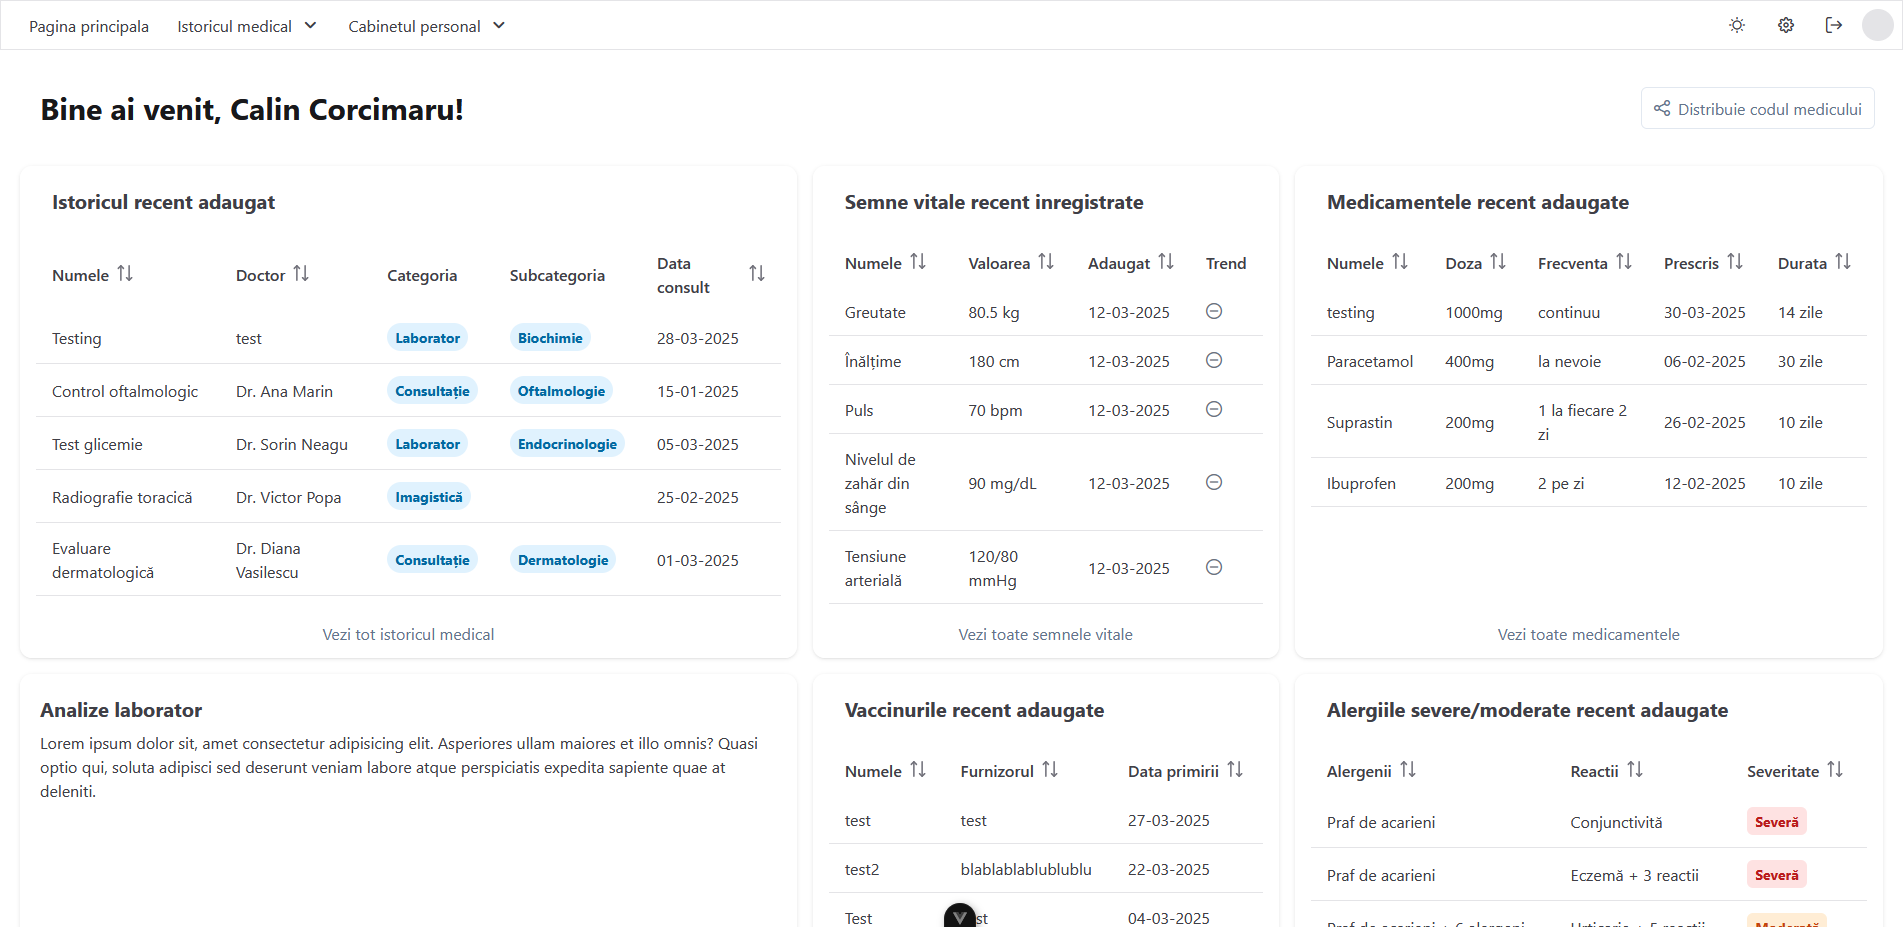
\includegraphics[width=\textwidth]{Desktop_DashboardView_Updated.png}
  \caption{Updated Dashboard View based on stakeholder feedback}\label{fig:dashboardchanges}
\end{figure}

\FloatBarrier{}

\subsection{Challenges}

The main challenge encountered in this sprint was actually not related to the project itself. Instead, the biggest challenge that was presented in this sprint was sickness, which led to the student being unable to work on the project for a week. This limited the amount of work that could be done in this sprint, leading to some of the preparatory work that was planned for this sprint to be moved to the next one.

\subsection{Requirements completed}

\begin{itemize}
  \item The system must allow the patient to specify and categorise the type of document they are uploading (lab test, doctor consultation, etc).
  \item The system must allow patients to upload their own medical records in a variety of formats (PDF, DOC, etc).
  \item The system must display the patient's history in a chronological order in the form of a timeline.
  \item When viewing doctor consultations, the system should divide them into categories based on the domain of the doctor (cardiology, neurology, etc).
  \item The system must allow the patient to add a description of the document they are uploading.
  \item The system should allow the patient to add a date for the document they are uploading.
  \item The system should allow the patient to add a location for the document they are uploading.
  \item The system should allow the patient to add the doctor name for the document they are uploading.
  \item The system should allow the patient to sort and filter the documents based on the type of document, date, location, and doctor name. 
\end{itemize}

\section{Sprint \#5}

The fifth sprint of the project was focused on adding the ability to add lab tests and extract the lab result values from those documents. The lab results would've been extracted by using a multimodal LLM, which would allow the system to precisely collect the lab results alongside other information such as units, reference ranges, etc without any additional human or system intervention. Using a MLLM would also simplify the extraction as the model would be able to export the results in an easily parseable response, such as JSON, which could be then used to display the information on the frontend or be processed in the backend. This feature was probably one of the most important ones in the whole system, as it represented an innovative way of automating the collection and storage of lab results for patients.  

This feature was a continuation of the work done in the previous sprint, as the lab tests were also part of the health records feature. As such, some of the initial work was done on top of existing components, which made development easier and faster. The feature was developed as per the initially agreed requirements and wireframes, with some changes to how the lab results were displayed on the frontend.

The sequence diagram for the lab tests extraction can be seen below in figure~. The diagram shows how the user interacts with the system to upload a lab test, how the system processes the file and sends it to the MLLM API, and how the response is then displayed to the user.

\begin{figure}[htbp]
  \centering
  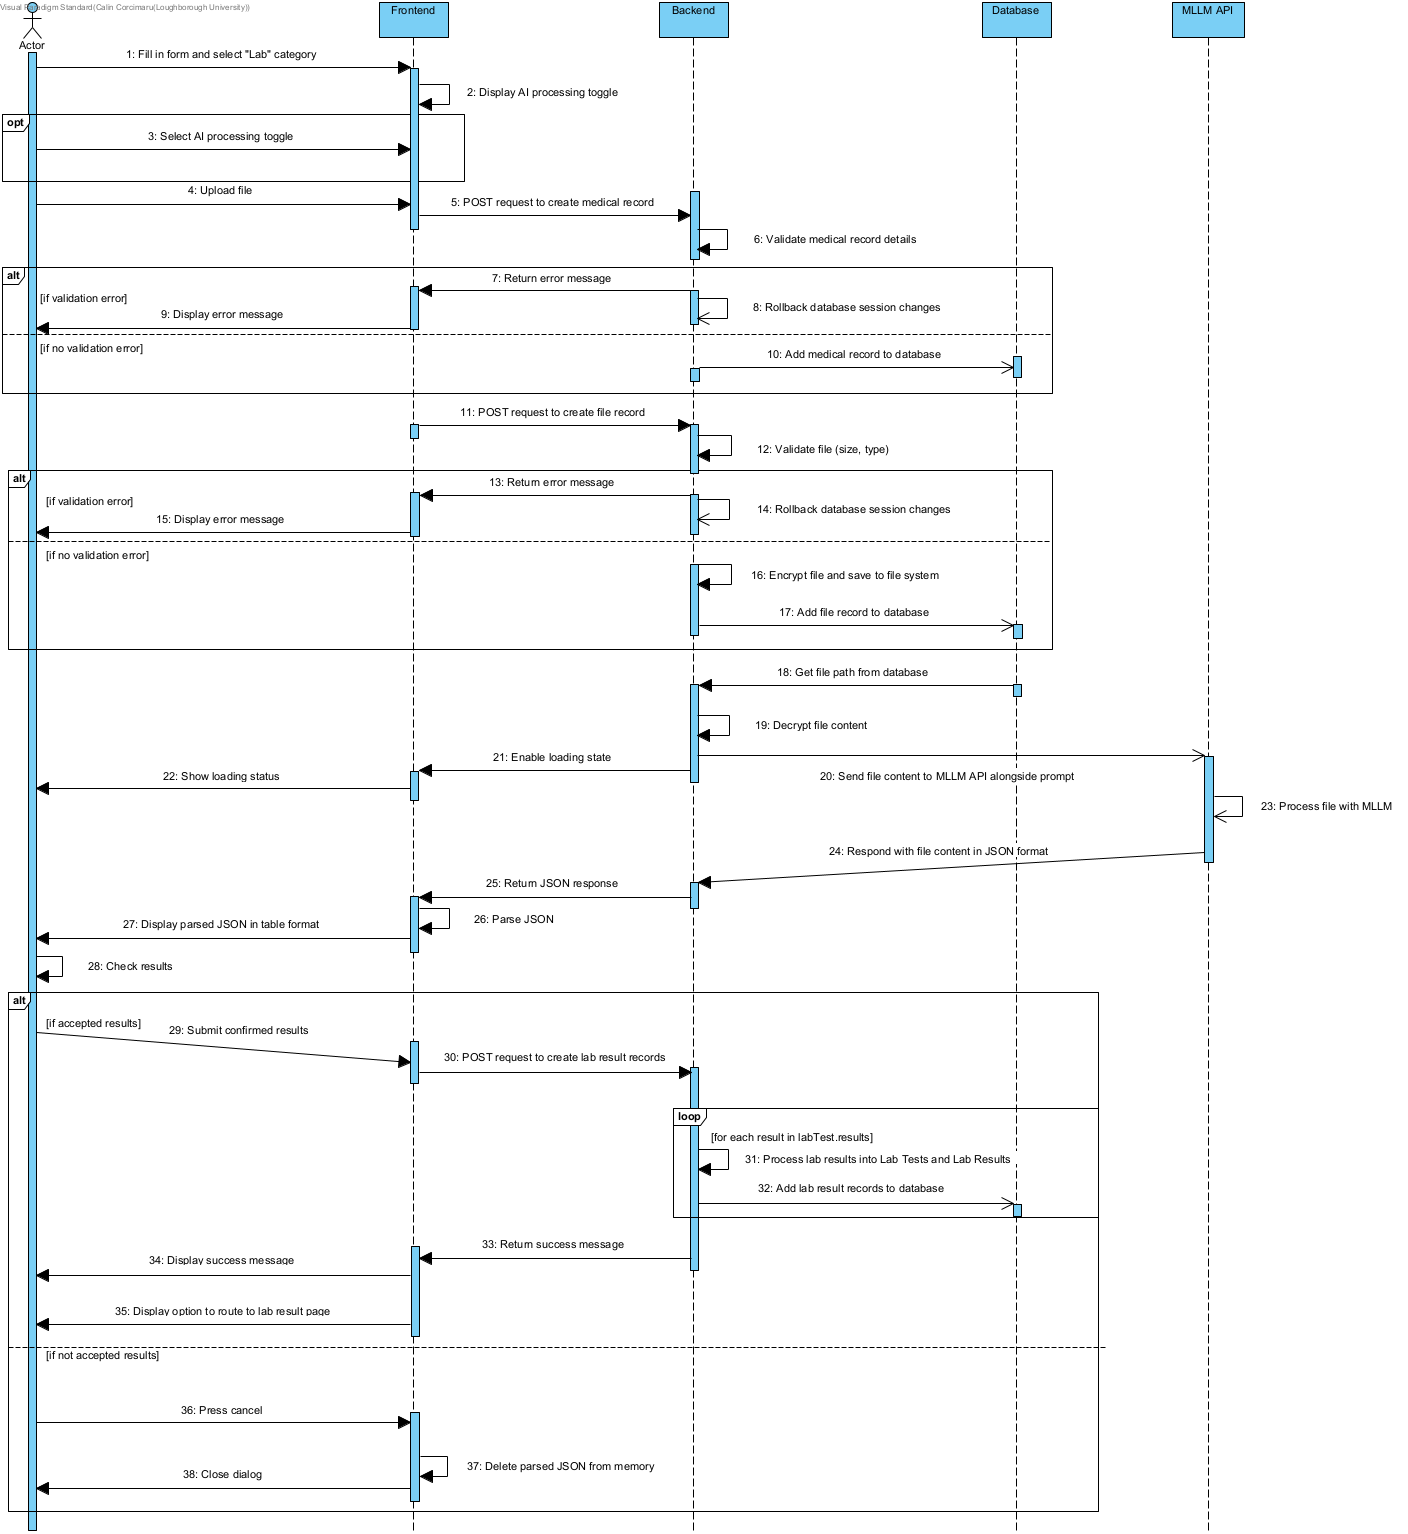
\includegraphics[width=\textwidth,height=0.8\textheight,keepaspectratio]{Sequence_lab.png}
  \caption{UML Sequence Diagram --- Extracting Lab Results}\label{fig:sequence_lab}
\end{figure}

\subsection{Lab Tests Extraction}

As lab tests were previously added in sprint \#4 as a health record, it was decided to use the existing `Add Health Record' component to allow the user to choose whether they'd like to extract the lab results besides uploading the file to the system. The decision was made to streamline the user experience of adding new health records, as the user would not have to go through multiple steps to add a lab test, but also because it would speed up development time as an existing component could be reused and made more feature-rich. Finally, this also closely matched the initial wireframe design for the `New Document' dialog, which can be seen in figure~\ref{fig:newDoc_wireframe}.

The updated dialog can be seen below in figure~\ref{fig:labs_addDoc}. The main change that can be seen is the addition of a toggle switch, which is displayed only when the user selects a lab test as the document type. If used, the toggle would still send the lab file to the backend and save it as a health record, but in addition to this, it would also send it to the MLLM API to be processed. 

\begin{figure}[ht]
  \centering
  \subfloat[Desktop version]{%
      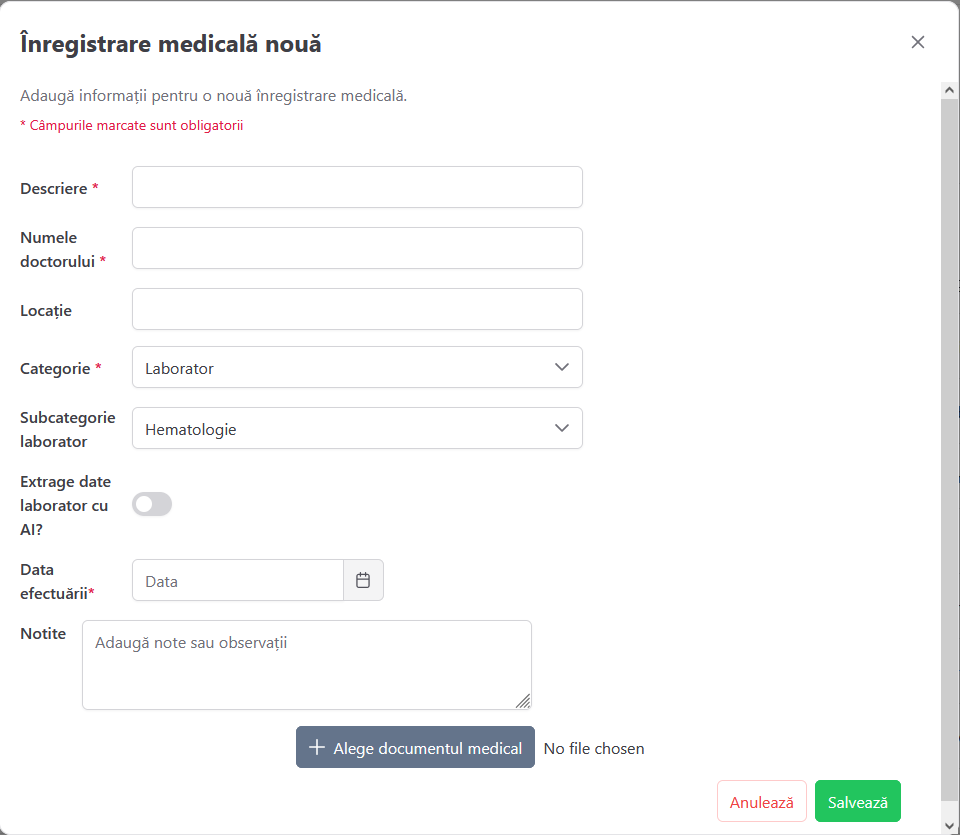
\includegraphics[width=0.7\textwidth]{Desktop_AddDoc_Labs.png}%
  }
  \\[\baselineskip]
  \subfloat[Mobile version]{%
      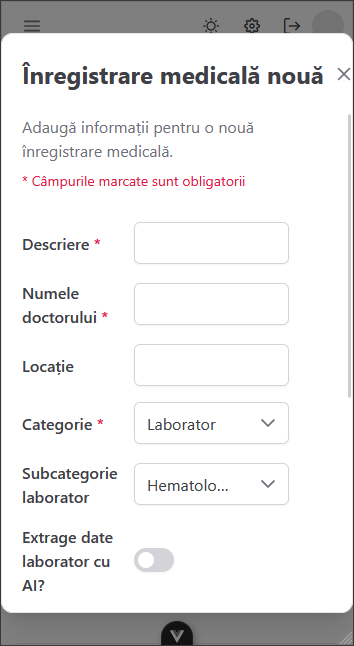
\includegraphics[width=0.3\textwidth]{Mobile_AddDoc_Labs.png}%
  }
  \caption{Desktop and Mobile version of the new Add Document dialog}\label{fig:labs_addDoc}
\end{figure}

\FloatBarrier{}

After the record is created and file is uploaded, the backend would find the file and send it the MLLM API\@. This was done to avoid uploading the file twice and to ensure the file would be successfully uploaded to the system before sending to the API\@.

The MLLM chosen for this project was Google's Gemini 2.0 Flash, which, as of writing this section, is part of the newly released family of Gemini models \parencite{gemini2}\@. The choice was made based on the list of available MLLMs that can be accessed via APIs with a free tier from table~\ref{tab:llm_apis}. Besides Google's AI Studio, none of the API providers allowed the uploading and processing of files, which made Gemini 2.0 Flash the most suitable choice for the project. It was noted that a local MLLM could've also been used for the project, a point which will be discussed in more detail in section~\ref{sec:future_work}.

Because an API was used, most of the work with the MLLM involved using Prompt Engineering techniques to ensure the model would process and return the data in the desired format. Prompting techniques from previous section~\ref{sec:prompt} were used to write the following prompt that was used to extract the lab results from the file:

\begin{lstlisting}[language=Python, caption=Prompt for Lab Results Extraction]

def extract_with_llm(file_content: bytes, file_type: str):
  prompt = """
  You have been given a document that contains lab results that is written in the Romanian language. Your job is to extract all lab results from this document in JSON format with the following fields: test_name, test_code, value, unit, reference_range, method. Sometimes the code of the test will be in the name itself, and it is your job to determine if the code is there, for example in brackets or separated by a comma, and separate the name and the code. Sometimes the lab result will not have a method specified, and in that case you return an empty string. The document is in Romanian, however the JSON keys should be in English.

  EXTREMELY IMPORTANT FORMATTING INSTRUCTIONS:
  1. Return ONLY the raw JSON array
  2. DO NOT use code blocks, backticks, or markdown formatting
  3. DO NOT include ```json or ``` anywhere in your response
  4. DO NOT include any explanations or text before or after the JSON
  5. Your response must start with the '[' character and end with the ']' character
  6. The output should be valid JSON that can be parsed directly
  7. Use period (.) as the decimal separator, not comma (,)

  Example of how your output should look, starting from the very first character:
  [{"test_name":"Hemoglobina","test_code":"HGB","value":"14.3","unit":"mg/dL","reference_range":"13.2-17.3", "method":"Chemiluminiscenta"}]
  
  if there is no method specified, return an empty string:
  [{"test_name":"Hemoglobina","test_code":"HGB","value":"14.3","unit":"mg/dL","reference_range":"13.2-17.3", "method":" "}]
  """
  
  response = client.models.generate_content(
      model="gemini-2.0-flash",
      contents=[prompt,
              types.Part.from_bytes(
              data=file_content, 
              mime_type=file_type
              )
          ])
  
  return response.text
  
\end{lstlisting}

The response from the API would be a JSON array containing all the lab results extracted from the document. Before saving, it is important to make sure the results and their values are correct. As such, it was decided to display all the extracted results back to the user in a PrimeVue DataTable component, which allowed for easy filtering of the results, but also for row-based editing. This way, the user could easily edit the values or remove any unwanted results before saving them to the system. An example of how the extracted lab results dialog looks can be seen below in figure~\ref{fig:labs_extracted}.

\begin{figure}[htbp]
  \centering
  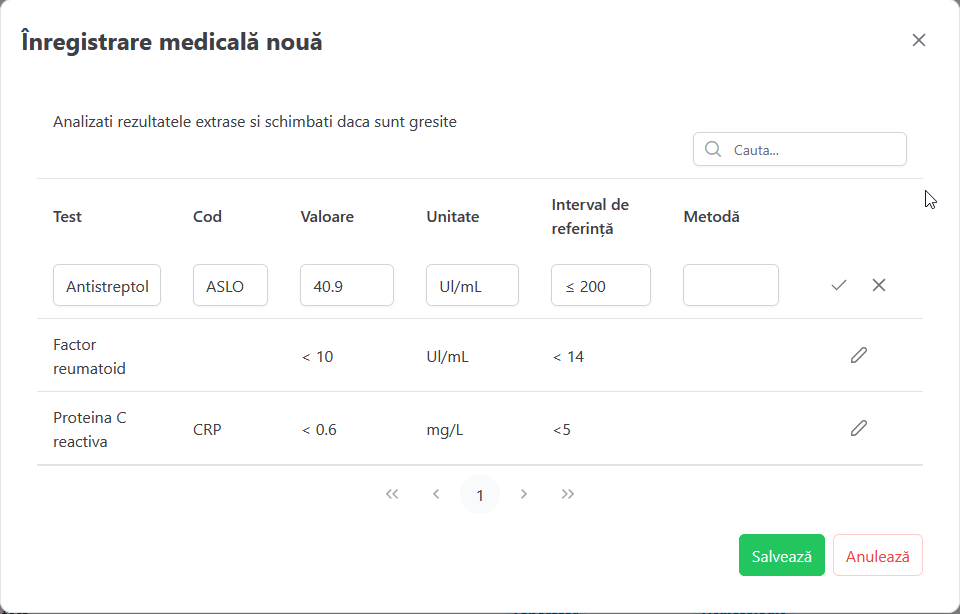
\includegraphics[width=\textwidth]{Desktop_Validate_Labs.png}
  \caption{Desktop dialog validation of extracted lab results}\label{fig:labs_extracted}
\end{figure}

A benefit of using PrimeVue's DataTables was not only its row editing feature or its filtering options, but also its ability to dynamically create columns based on the data received. This was perfect for the lab results, as it is not possible to know beforehand how many results will be extracted from a document. A code snippet of the DataTable can be seen below:

\begin{lstlisting}[language=HTML, caption=Dynamic DataTable for Lab Results]
  <DataTable
    :value="extractionResult"
    v-model:editingRows="editingRows"
    class="w-full"
    :rows="10"
    editMode="row"
    paginator
    dataKey="test_name"
    @row-edit-save="onRowEditSave"
    v-model:filters="filters"
    :globalFilterFields="['test_name', 'test_code']"
  >
    <template #header>
      <h2 class="m-0">Analizati rezultatele extrase si schimbati daca sunt gresite</h2>
      <div class="flex justify-end">
        <IconField>
          <InputIcon>
            <i class="pi pi-search" />
          </InputIcon>
          <InputText
            size="small"
            v-model="filters['global'].value"
            placeholder="Cauta..."
          />
        </IconField>
      </div>
    </template>
    <Column 
      v-for="col of columns" 
      :key="col.field" 
      :field="col.field" 
      :header="col.header"
    >
      <template #editor="{ data, field }">
        <InputText v-model="data[field]" class="w-full" fluid />
      </template>
    </Column>
    <Column
      :rowEditor="true"
      style="width: 10%; min-width: 8rem"
      bodyStyle="text-align:center"
    />
  </DataTable>
\end{lstlisting}

After confirming the extracted test results, they are processed and saved to the backend. The next subsection will discuss in more detail how the backend was changed to accommodate the new lab tests and their results.

\subsubsection{Backend changes}

To supporrt the processing and addition to database for the newly extracted lab results, two new tables were created in the database: LabTest and LabResult. The decision to use 2 tables was made to avoid duplication of data for fields like name and code of the lab test, as these would be common for all the lab results, regardless of their method or machinery used. This would also prove beneficial as multiple results could be assigned to one test, making the tracking and display of the historical results much easier. Finally, by having 2 separate tables, LabTests could be dynamically populated with new tests straight from uploaded documents, without the need for manual addition or creation of test types. The updated database schema can be seen below in figure~\ref{fig:erd_s5}.

\noindent\begin{minipage}{\textwidth}
  \begin{center}
      \rotatebox[origin=c]{270}{
          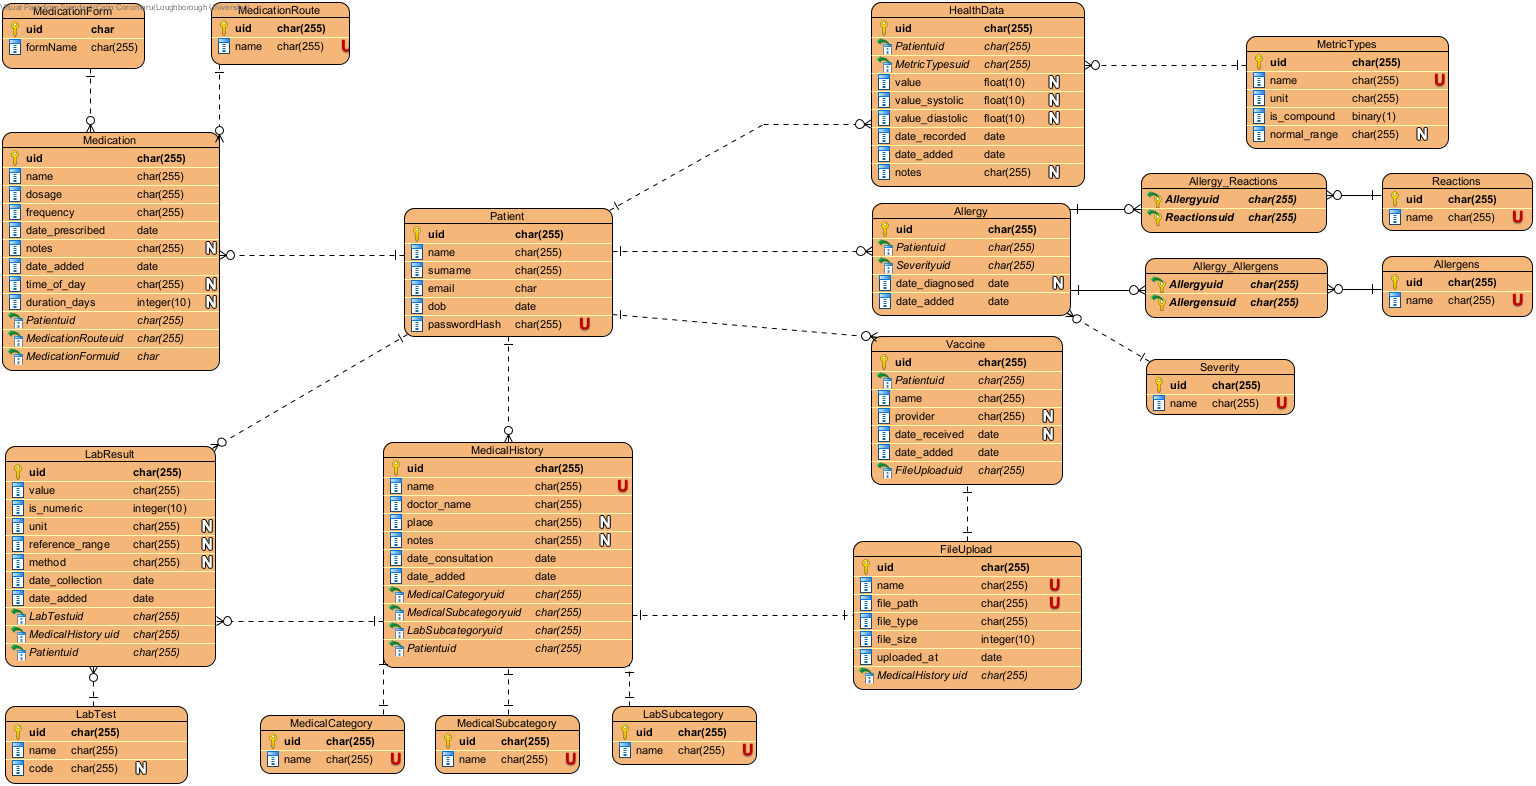
\includegraphics[width=0.95\textheight,keepaspectratio]{ERD_updatedS5.png}
      }
      \captionof{figure}{Updated Entity Relationship Diagram \- Sprint \#5}\label{fig:erd_s5}
  \end{center}
\end{minipage}

\FloatBarrier{}

As can be seen by the diagram above, there might seem to be a redundant relationship between the Patient and LabResult tables, as LabResult is already related to MedicalHistory, which in turn is related to a Patient. However, the decision was made to introduce the relationship as it would allow for easier querying when getting all the lab results for a patient, in the case of the dashboard view or even in the next sprint when the share functionality is added.

Similarly, a code snippet of the endpoint that handles the creation of lab results can be seen below:

\begin{lstlisting}[language=Python, caption=Lab Results Endpoint]
  # Create the lab test records in the database
@router.post('/me/labtests/')
async def create_lab_tests(extraction_result: LabsCreate, user_id: uuid.UUID = Depends(validate_session), session: Session = Depends(get_session)):
    medhistory = session.get(MedicalHistory, extraction_result.medicalhistory_id)
    user = session.get(User, user_id)
    
    if not medhistory:
        raise HTTPException(status_code=status.HTTP_404_NOT_FOUND, detail="Medical history not found")
    
    if medhistory.user_id != user_id:
        raise HTTPException(status_code=status.HTTP_403_FORBIDDEN, detail="Not authorized to access this medical history")
    
    for lab_item in extraction_result.lab_tests:
        lab_test = session.exec(select(LabTest).where(LabTest.name == lab_item.name)).first()
        
        if not lab_test:
            lab_test = LabTest(
                name = lab_item.name,
                code = lab_item.code,
            )
            session.add(lab_test)
            session.flush()
        
        lab_result = LabResult(
            value = lab_item.value,
            is_numeric = check_is_numeric(lab_item.value),
            unit = lab_item.unit,
            reference_range = lab_item.reference_range,
            date_collection = extraction_result.date_collection,
            test = lab_test,
            medicalhistory = medhistory,
            user = user,
            method = lab_item.method
        )
        
        session.add(lab_result)
        session.flush()
        
        # TODO: Maybe later have an array to store the lab results and return them all at once
        
    session.commit()
    
    return {
        "status": status.HTTP_201_CREATED,
        "message": "Lab tests created successfully"
        }
\end{lstlisting}

\subsection{Lab Results Display}

The final part of the work on the lab extraction feature was the display of said results within their own page in the system. The initial idea was to reuse the existing design from the vitals page, which can be seen in figures~\ref{fig:vitalspage},~\ref{fig:vitalspagegraph} and~\ref{fig:vitalchanges}. This would've also followed the initially agreed wireframes and design. 

However, upon discussing with stakeholders, an idea and request to change the design was floated in the meeting: instead of using the design from vitals page, the idea was to display everything in a tabular format where rows could be expanded to show the historical resutls from that specific test. This is where the division into 2 tables in the database played an important role: LabTest could be used as the `parent' element in the table, which could be sorted and filtered, while the LabResult elements would only be shown if the row would be expanded in the table. 

This idea was eventually accepted, as it would allow for a more compact view of the lab results, easier filtering/sorting and it enabled for a way to display the most recent results for each test as a separate column without being intrusive. The results were sorted by date in the backend already, which allowed for the most recent results to be easily selected and displayed. Finally, instead of using a big graph that might take up a lot of space on the page, it was decided to use a small graph, also known as a sparkline, which would only show the trend of the results over time, based on their reference range and collection date. Colors such as red and green were used to indicate whether the results were within the normal range or outside of it. An example of how the new lab results page looks can be seen below in figure~\ref{fig:labs_page} and~\ref{fig:labs_page_mobile}.

\begin{figure}[ht]
  \centering
  \subfloat[Desktop version]{%
      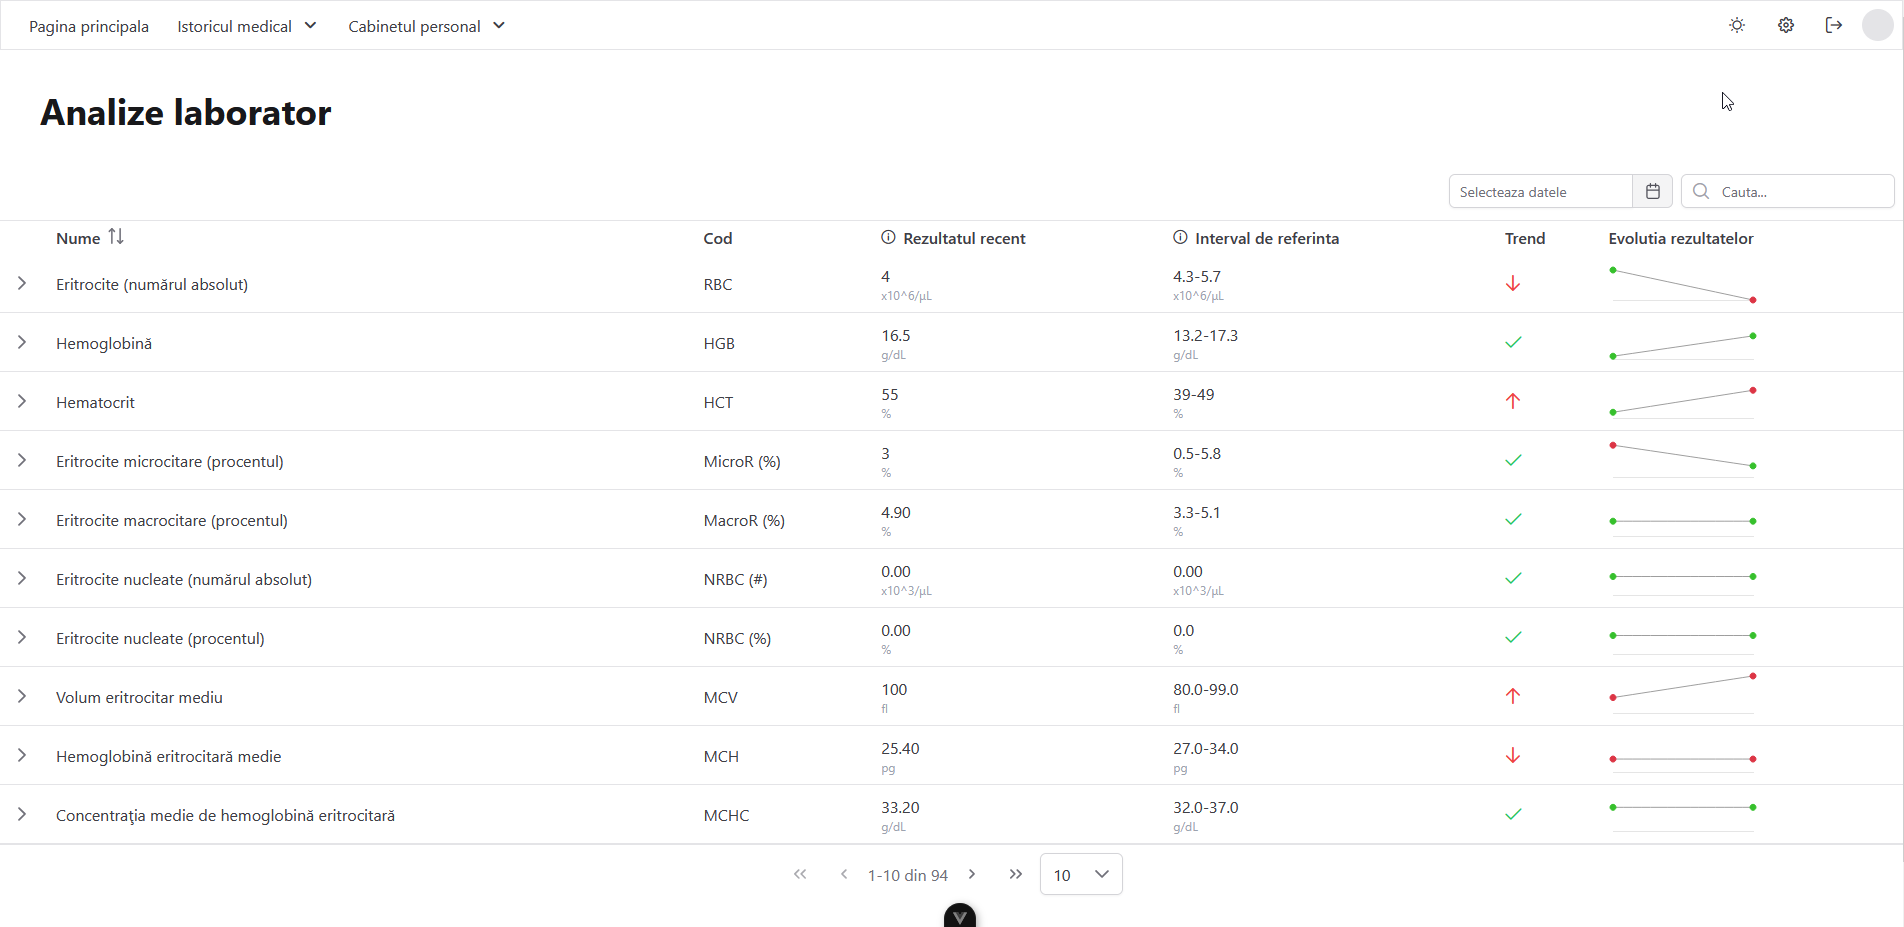
\includegraphics[width=0.9\textwidth]{Desktop_LabView.png}%
  }
  \\[\baselineskip]
  \subfloat[Desktop version \#2]{%
      \includegraphics[width=0.9\textwidth]{Desktop_LabView2.png}%
  }
  \caption{Desktop version of the new Lab View page}\label{fig:labs_page}
\end{figure}

\FloatBarrier{}

\begin{figure}[ht]
  \centering
  \subfloat[Mobile version]{%
      \includegraphics[width=0.4\textwidth]{Mobile_LabView.png}%
  }
  \hfill
  \subfloat[Mobile version \#2]{%
      \includegraphics[width=0.4\textwidth]{Mobile_LabView2.png}%
  }
  \caption{Mobile version of the new Lab View page}\label{fig:labs_page_mobile}
\end{figure}

\FloatBarrier{}

% TODO: Add screenshots and talk about the dashboard component, which I actually forgot to make

\subsection{Challenges encountered}

This sprint encountered less challenges than the previous ones, meaning that the work was able to be done faster than it was initially planned. However, there were still some challenges that were encountered during the development of the lab tests extraction feature.

One of the biggest challenges was the change in design for the lab results page. Even though the initial design was agreed upon before the development begun, the stakeholders insisted on the change in design, which added a slight overhead in the form of additional design and research on how to implement the new idea. However, it must be noted that the new design also allowed for an easier development experience as a lot of the work was done by PrimeVue's DataTable component, which ultimately sped up the completion of the feature. Ultimately, the agility of the development process allowed for the change to be made without any major issues, an idea which will be further discussed in section~\ref{sec:future_work}.

The other challenge was the time pressure, as the student was nearing the deadline of the project. This meant that the focus was on implementing only the most necessary and basic features, without any space for creative or innovative ideas.

\subsection{Requirements completed}

\begin{itemize}
  \item The system must provide an overview of the patient history through 3 main sections: personal information, lab tests, and doctor consultations.
  \item The system must allow the doctor to view blood tests in a graphical format.
  \item The system must allow the doctor to view blood tests in a numerical, tabular format.
  \item The system must allow the doctor to view the patient's history in a chronological order.
  \item For blood test results, the system should display the normal range values for each test.
  \item The system could allow the patient to switch between viewing the lab tests in the document format or in a tabular, numerical format.
\end{itemize}

\section{Sprint \#6}

\chapter{Evaluation}

\section{Deployment}

\section{System Testing}

\section{User Acceptance Testing}

\section{Client feedback}

\chapter{Conclusion and Future Work}

\section{Areas of Improvement}

\section{Future Work}

\section{Lessons Learned and Reflections}

\section{Final Thoughts}

% Rename Bibliography to References
%\renewcommand\bibname{References}
\printbibliography[heading=bibintoc, title={References}]

\appendix

\chapter{Requirements}\label{sec:requirements}

% TODO: Revisit requirements and add more details

\begin{table}[h!]
    \centering
    \begin{tabular}{|c|p{10cm}|c|}
    \hline
    \textbf{ID}  & \textbf{Requirement}  & \textbf{Priority} \\ \hline
    1.1  & The system must be accessible on all modern desktop and mobile-based browsers.       & Must Have \\ \hline
    1.2  & The system must be accessible from any location by using an internet connection.     & Must Have \\ \hline
    1.3  & The system must store the data in a secure manner, ensuring that only the patient and the doctor can access the data. & Must Have \\ \hline
    1.4  & When shared with the doctor via a link, the system must load within 3 to 5 seconds when accessed via a desktop browser. & Should Have \\ \hline
    1.5  & When shared with the doctor via a link, the system should secure the data with a unique token or PIN that expires after the specified time frame. & Could Have \\ \hline
    1.6  & The system could be accessible on all modern mobile devices via a mobile application. & Could Have \\ \hline
    \end{tabular}
    \caption{Non-functional Requirements}
\end{table}
    
\begin{table}[h!]
    \centering
    \begin{tabular}{|c|p{10cm}|c|}
    \hline
    \textbf{ID}  & \textbf{Requirement}  & \textbf{Priority} \\ \hline
    2.1  & The system must provide a secure login mechanism for patients by using a combination of login and password. & Must Have \\ \hline
    2.2 & The database must store the user credentials in a secure manner. & Must Have \\ \hline
    2.3 & The system could provide an option for multi factor authentication. & Could Have \\ \hline
    2.4 & The system could provide an option for password recovery. & Could Have \\ \hline
    2.5  & If used on mobile, the system could allow the patient to use biometric authentication for logging in. & Should Have \\ \hline
    \end{tabular}
    \caption{Login Requirements}
\end{table}

\begin{table}[h!]
    \centering
    \begin{tabular}{|c|p{10cm}|c|}
    \hline
    \textbf{ID}  & \textbf{Requirement}  & \textbf{Priority} \\ \hline
    3.1  & The system must allow patients to upload their own medical records in a variety of formats (PDF, DOC, etc). & Must Have \\ \hline
    3.2 & The system should allow to upload files/documents for other types of records (vaccine certificates, etc). & Should Have \\ \hline
    3.2  & The system must allow the patient to specify and categorise the type of document they are uploading (lab test, doctor consultation, etc). & Must Have \\ \hline
    3.3 & The system must allow the patient to add a description of the document they are uploading. & Must Have \\ \hline
    3.4 & The system should allow the patient to add a date for the document they are uploading. & Should Have \\ \hline
    3.5 & The system should allow the patient to add a location for the document they are uploading. & Should Have \\ \hline
    3.6 & The system should allow the patient to add the doctor name for the document they are uploading. & Should Have \\ \hline
    3.7 & The system should allow the patient to sort and filter the documents based on the type of document, date, location, and doctor name. & Should Have \\ \hline
    3.8 & If used on mobile, the system should allow the patient to take a picture of the document and upload it. & Could Have \\ \hline
    \end{tabular}
    \caption{Document Upload Requirements}
\end{table}

\begin{table}[h!]
    \centering
    \begin{tabular}{|c|p{10cm}|c|}
    \hline
    \textbf{ID}  & \textbf{Requirement}  & \textbf{Priority} \\ \hline
    4.1  & The system must allow the patient to generate a shareable link to provide access to their medical records. & Must Have \\ \hline
    4.2  & When creating the shareable link, the system must allow the patient to set an expiration date for the link. & Must Have \\ \hline
    4.3  & When creating the shareable link, the system should allow the patient to set an access password for the link. & Should Have \\ \hline
    4.4  & When creating the shareable link, the system should allow the patient to select which records to share with the doctor. & Should Have \\ \hline
    \end{tabular}
    \caption{Patient Shareable Link Requirements}
\end{table}

\begin{table}[h!]
    \centering
    \begin{tabular}{|c|p{10cm}|c|}
    \hline
    \textbf{ID}  & \textbf{Requirement}  & \textbf{Priority} \\ \hline
    5.1  & The patient personal cabinet must provide an overview of the patient's history through 3 main sections: personal information, lab tests, and doctor consultations. & Must Have \\ \hline
    5.2  & The system must display the patient's history in a chronological order in the form of a timeline. & Must Have \\ \hline
    5.3 & The system must have a dashboard view which displays an overview of the most recent information added to the system (latest lab tests, doctor consultations, vaccinations etc). & Must Have \\ \hline
    5.4  & The system must allow patients to add their own personal information, such as name or date of birth. & Must Have \\ \hline
    5.5  & The system must allow the patient to add their own allergies. & Must Have \\ \hline
    5.6  & The system must allow the patient to add their own vaccinations. & Must Have \\ \hline
    5.7  & When viewing doctor consultations, the system should divide them into categories based on the domain of the doctor (cardiology, neurology, etc). & Should Have \\ \hline
    5.8  & The system should allow the patient to enter vitals information, such as height, weight, blood pressure, etc. & Should Have \\ \hline
    5.9  & The system should display the information in both a list or grid view. & Should Have \\ \hline
    5.10  & When multiple vital entries are made, the system could display a historical graph of the patient's vitals. & Could Have \\ \hline
    5.11 & The system could allow the patient to switch between viewing the lab tests in the document format or in a tabular, numerical format. & Could Have \\ \hline
    \end{tabular}
    \caption{Patient Personal Cabinet Requirements}
\end{table}

\begin{table}[h!]
    \centering
    \begin{tabular}{|c|p{10cm}|c|}
    \hline
    \textbf{ID}  & \textbf{Requirement}  & \textbf{Priority} \\ \hline
    6.1  & The system must provide an overview of the patient history through 3 main sections: personal information, lab tests, and doctor consultations. & Must Have \\ \hline
    6.2  & When shared with the doctor, the system must allow the doctor to only view the patient's history, not edit it. & Must Have \\ \hline
    6.3  & The system must allow the doctor to view blood tests in a graphical format. & Must Have \\ \hline
    6.4  & The system must allow the doctor to view blood tests in a numerical, tabular format. & Must Have \\ \hline
    6.5  & The system must allow the doctor to view the patient's history in a chronological order. & Must Have \\ \hline
    6.6  & The system must display the doctor consultation and every lab test, except for blood tests, in a free text or document format. & Must Have \\ \hline
    6.7  & When viewing blood test results, the system should show the source document of the blood test value. & Should Have \\ \hline
    6.8  & For blood test results, the system should display the normal range values for each test. & Should Have \\ \hline
    \end{tabular}
    \caption{Shared Patient Information Requirements (Doctor View)}
\end{table}

\begin{table}[h!]
    \centering
    \begin{tabular}{|c|p{10cm}|c|}
    \hline
    \textbf{ID}  & \textbf{Requirement}  & \textbf{Priority} \\ \hline
    7.1  & The system must allow patients to enter their current medication including details such as the name of the drug, dosage, frequency and start/end date. & Must Have \\ \hline
    7.2 & The system must allow patients to add new medication to their list. & Must Have \\ \hline
    7.3 & When adding medication, the system should have 2 options: add a simplified version of the medication or add a detailed version of the medication. & Should Have \\ \hline
    7.4 & When choosing the simplified version, the system should allow the patient to just add the name, dosage and duration of the medication. & Should Have \\ \hline
    7.5 & When choosing the detailed version, the system should allow the patient to add the name, dosage, frequency, start/end date, and the reason for taking the medication. & Should Have \\ \hline
    7.6  & The system should allow patients to add their past medication & Should Have \\ \hline
    7.7  & The system should allow patients to set medication reminders. & Should Have \\ \hline
    7.8 & After entering the medication, the system could allow the patient to track the medication intake. & Could Have \\ \hline

    \end{tabular}
    \caption{Patient Medication Requirements}
\end{table}

\chapter{Wireframes}\label{sec:wireframes}

\begin{figure}[ht]
    \centering
    \subfloat[Desktop version]{%
        \includegraphics[width=0.75\textwidth]{wireframes/Desktop_dashboard.png}%
    }
    \hspace{0.05\textwidth}
    \subfloat[Mobile version]{%
        \includegraphics[scale=0.25]{wireframes/Mobile_dashboard.png}%
    }
    \caption{Desktop and Mobile version of the Dashboard screen}
\end{figure}

\begin{figure}[ht]
    \centering
    \subfloat[Desktop version]{%
        \includegraphics[width=0.75\textwidth]{wireframes/Desktop_doctorView.png}%
    }
    \hspace{0.05\textwidth}
    \subfloat[Mobile version]{%
        \includegraphics[scale=0.3]{wireframes/Mobile_dashboardMenu.png}%
    }
    \caption{Desktop and Mobile version of the Doctor View screen}
\end{figure}

\begin{figure}[ht]
    \centering
    \subfloat[Desktop version]{%
        \includegraphics[width=0.75\textwidth]{wireframes/Desktop_labTest.png}%
    }
    \hspace{0.05\textwidth}
    \subfloat[Mobile version]{%
        \includegraphics[scale=0.3]{wireframes/Mobile_labTest.png}%
    }
    \caption{Desktop and Mobile version of the Lab Test screen}
\end{figure}

\begin{figure}[ht]
    \centering
    \subfloat[Desktop version]{%
        \includegraphics[width=0.75\textwidth]{wireframes/Desktop_medHistory.png}%
    }
    \hspace{0.05\textwidth}
    \subfloat[Mobile version]{%
        \includegraphics[scale=0.3]{wireframes/Mobile_medHistory.png}%
    }
    \caption{Desktop and Mobile version of the Medical History screen}
\end{figure}

\begin{figure}[ht]
    \centering
    \subfloat[Desktop version]{%
        \includegraphics[width=0.75\textwidth]{wireframes/Desktop_newDoc.png}%
    }
    \hspace{0.05\textwidth}
    \subfloat[Mobile version]{%
        \includegraphics[scale=0.3]{wireframes/Mobile_newDoc.png}%
    }
    \caption{Desktop and Mobile version of the New Document screen}
\end{figure}

\begin{figure}[ht]
    \centering
    \subfloat[Desktop version]{%
        \includegraphics[width=0.75\textwidth]{wireframes/Desktop_shareDoctor.png}%
    }
    \hspace{0.05\textwidth}
    \subfloat[Mobile version]{%
        \includegraphics[scale=0.3]{wireframes/Mobile_shareDoctor.png}%
    }
    \caption{Desktop and Mobile version of the Share Doctor screen}
\end{figure}

\begin{figure}[ht]
    \centering
    \subfloat[Desktop version]{%
        \includegraphics[width=0.75\textwidth]{wireframes/AI-allergies-desktop.png}%
    }
    \hspace{0.05\textwidth}
    \subfloat[Mobile version]{%
        \includegraphics[scale=0.3]{wireframes/Mobile_allergies.png}%
    }
    \caption{Desktop and Mobile version of the Allergies screen}
\end{figure}

\begin{figure}[ht]
    \centering
    \includegraphics[width=0.3\textwidth]{wireframes/Mobile_vaccines.png}
    \caption{Mobile version of the Vaccines screen}
\end{figure}

% Include appendix section if needed
%\include{Appendix/Appendix}

\end{document}